\documentclass[12pt]{scrartcl}

\usepackage[T1]{fontenc}
\usepackage[utf8]{inputenc}
\usepackage{amsmath}
\usepackage{amsfonts}
\usepackage{amssymb}
\usepackage{amsbsy}
\usepackage{graphicx}
\usepackage{float}
\usepackage{array}
\usepackage{booktabs}
\usepackage{multirow}
\usepackage{bm}
\usepackage{verbatim}
\usepackage[english]{babel}
\usepackage{color}
\usepackage{url}
\usepackage{fancybox}
\usepackage[stable]{footmisc}
\usepackage[format=plain,labelfont=bf]{caption}
\usepackage{fancyhdr}
\usepackage{natbib}
\usepackage{calc}
\usepackage{textcomp}
\usepackage[pdftex,pdfborder={0 0 0}]{hyperref}
\usepackage{pdfpages}
\usepackage{tikz}
\usetikzlibrary{shapes,backgrounds,fit,positioning,arrows,positioning,decorations.pathmorphing,decorations.pathreplacing,backgrounds}
\usepackage{accents}

\renewcommand*{\familydefault}{\sfdefault}

% Margins
\addtolength{\textheight}{1.0cm}
\addtolength{\oddsidemargin}{-0.5cm}
\addtolength{\evensidemargin}{-0.5cm}
\addtolength{\textwidth}{1.0cm}
\parindent=0em

% New math commands
\newcommand{\overbar}[1]{\mkern 1.5mu\overline{\mkern-1.5mu#1\mkern-1.5mu}\mkern 1.5mu}
\DeclareMathOperator{\diag}{diag}
\DeclareMathOperator{\Diag}{Diag}
\DeclareMathOperator{\tr}{tr}
\DeclareMathOperator{\var}{var}
\DeclareMathOperator{\Cov}{Cov}
\DeclareMathOperator{\Cor}{Cor}
\newcommand\independent{\protect\mathpalette{\protect\independenT}{\perp}}
\def\independenT#1#2{\mathrel{\setbox0\hbox{$#1#2$}%
\copy0\kern-\wd0\mkern4mu\box0}}

% Appropriate font for \mathcal{}
\DeclareSymbolFont{cmmathcal}{OMS}{cmsy}{m}{n}
\DeclareSymbolFontAlphabet{\mathcal}{cmmathcal}

% Set subscript and superscripts positions
\everymath{
\fontdimen13\textfont2=5pt
\fontdimen14\textfont2=5pt
\fontdimen15\textfont2=5pt
\fontdimen16\textfont2=5pt
\fontdimen17\textfont2=5pt
}

% Bibliography style
\setlength{\bibsep}{1pt}

% Part
\renewcommand\partheadstartvskip{\clearpage\null\vfil}
\renewcommand\partheadmidvskip{\par\nobreak\vskip 20pt\thispagestyle{empty}}
\renewcommand\partheadendvskip{\vfil\clearpage}
\renewcommand\raggedpart{\centering}

\begin{document}
\title{Sample covariance filtering}
\author{Benjamin Ménétrier}
\date{Last update: \today}

\thispagestyle{empty}

\maketitle
\begin{center}
Copyright \copyright 2015-2024: UCAR, CERFACS, METEO-FRANCE, IRIT and Meteorologisk Institutt
\end{center}

\tableofcontents

\clearpage

\part{Sampling covariances}

\section{Standard estimators}

In this section, indices $i$, $j$, $k$ and $l$ refer to vector elements and indices $p$, $q$, $r$ and $s$ to ensemble members.

\subsection{Sampling error}
Let $\mathbf{x}^b \in \mathbb{R}^n$ be a random vector and $\boldsymbol{\varepsilon}^b$ its unbiased counterpart:
\begin{align}
\boldsymbol{\varepsilon}^b = \mathbf{x}^b - \mathbb{E} \left[\mathbf{x}^b\right]
\end{align}
where $\mathbb{E} [\cdot]$ denotes the statistical expectation. The covariance of the distribution of $\mathbf{x}^b$ is denoted $\mathbf{B} \in \mathbb{R}^{n \times n}$ and its fourth order centered moment is denoted $\boldsymbol{\Xi} \in \mathbb{R}^{n \times n \times n \times n}$. They are respectively given by:
\begin{subequations}
\begin{align}
\label{eq:cov}
B_{ij} & = \mathbb{E}\left[\varepsilon^b_i \varepsilon^b_j\right] \\
\label{eq:mom_4}
\Xi_{ijkl} & = \mathbb{E}\left[\varepsilon^b_i \varepsilon^b_j \varepsilon^b_k \varepsilon^b_l\right]
\end{align}
\end{subequations}
$  $\\
Let $\left\{\widetilde{\mathbf{x}}^b_1,\dots,\widetilde{\mathbf{x}}^b_N\right\}$ be a set of $N$ vectors that samples the distribution of $\mathbf{x}^b$ and $\left\{\delta \widetilde{\mathbf{x}}^b_1,\dots,\delta \widetilde{\mathbf{x}}^b_N\right\}$ their centered counterparts:
\begin{align}
\delta \widetilde{\mathbf{x}}^b_p = \widetilde{\mathbf{x}}^b_p - \langle \widetilde{\mathbf{x}}^b \rangle
\end{align}
where $\langle \cdot \rangle$ denotes the ensemble mean:
\begin{align}
\label{eq:exp_estim}
\langle \widetilde{\mathbf{x}}^b \rangle = \frac{1}{N} \sum_{p=1}^N \widetilde{\mathbf{x}}^b_p
\end{align}
Centered moments \eqref{eq:cov} et \eqref{eq:mom_4} can be estimated from these perturbations by:
\begin{subequations}
\begin{align}
\label{eq:cov_estim}
\widetilde{B}_{ij} & = \frac{1}{N-1} \sum_{p=1}^N \delta \widetilde{x}^b_{i,p} \delta \widetilde{x}^b_{j,p}  \\
\label{eq:mom_4_estim}
\widetilde{\Xi}_{ijkl} & = \frac{1}{N} \sum_{p=1}^N \delta \widetilde{x}^b_{i,p} \delta \widetilde{x}^b_{j,p} \delta \widetilde{x}^b_{k,p} \delta \widetilde{x}^b_{l,p}
\end{align}
\end{subequations}
$  $\\
If the ensemble size $N$ goes to infinity, asymptotic $\widetilde{\mathbf{B}}$ and $\widetilde{\boldsymbol{\Xi}}$ converge to $\mathbf{B}$ and $\boldsymbol{\Xi}$ respectively:
\begin{subequations}
\begin{align}
\lim_{N \rightarrow \infty} \widetilde{\mathbf{B}} & = \mathbf{B} \\
\lim_{N \rightarrow \infty} \widetilde{\boldsymbol{\Xi}} & = \boldsymbol{\Xi}
\end{align}
\end{subequations}
The sampling errors on $\widetilde{\mathbf{B}}$ and $\widetilde{\boldsymbol{\Xi}}$ are respectively defined by:
\begin{subequations}
\begin{align}
\widetilde{\mathbf{B}}^e & = \widetilde{\mathbf{B}} - \mathbf{B} \\
\widetilde{\boldsymbol{\Xi}}^e & = \widetilde{\boldsymbol{\Xi}} - \boldsymbol{\Xi}
\end{align}
\end{subequations}

\subsection{Expected sample mean}
Since $\mathbb{E} \left[\widetilde{\mathbf{x}}^b_p\right]$ is the same for any member index $p$, it is hereafter denoted $\mathbb{E} \left[\widetilde{\mathbf{x}}^b\right]$. Thus, the sample mean expectation is given by:
\begin{align}
\mathbb{E} \left[\langle \widetilde{\mathbf{x}}^b \rangle\right] & = \mathbb{E} \left[\frac{1}{N} \sum_{p=1}^N \widetilde{\mathbf{x}}^b_p\right] \nonumber \\
& = \frac{1}{N} \sum_{p=1}^N \mathbb{E} \left[\widetilde{\mathbf{x}}^b\right] \nonumber \\
& = \mathbb{E} \left[\widetilde{\mathbf{x}}^b\right]
\end{align}

\subsection{Covariance of sample means}
Since ensemble members are mutually independent, their covariance is:
\begin{align}
\Cov \left(\widetilde{x}^b_{i,p},\widetilde{x}^b_{j,q}\right) = \left\{
\begin{array}{cl}
B_{ij} & \text{ if }p=q \\
0 & \text{ if }p \ne q
\end{array}
\right.
\end{align}
Thus, the expected product of sample means is given by:
\begin{align}
\mathbb{E} \left[\langle \widetilde{x}^b_i \rangle \langle \widetilde{x}^b_j \rangle\right] = & \mathbb{E} \left[\left(\frac{1}{N} \sum_{p=1}^N \widetilde{x}^b_{i,p} \right) \left(\frac{1}{N} \sum_{q=1}^N \widetilde{x}^b_{j,q}\right)\right] \nonumber \\
= \ & \frac{1}{N^2} \sum_{1 \le p,q \le N} \mathbb{E} \left[\widetilde{x}^b_{i,p} \widetilde{x}^b_{j,q}\right] \nonumber \\
= \ & \frac{1}{N^2} \sum_{1 \le p,q \le N} \left(\Cov \left(\widetilde{x}^b_{i,p},\widetilde{x}^b_{j,q}\right)+\mathbb{E} \left[\widetilde{x}^b_i\right] \mathbb{E} \left[\widetilde{x}^b_j\right]\right) \nonumber \\
= \ & \frac{1}{N^2} \left(\sum_{p=1}^N \Cov \left(\widetilde{x}^b_{i,p},\widetilde{x}^b_{j,p}\right) + \sum_{\substack{1 \le p,q \le N\\p \ne q}} \Cov \left(\widetilde{x}^b_{i,p},\widetilde{x}^b_{j,q}\right) \right) + \mathbb{E} \left[\widetilde{x}^b_i\right] \mathbb{E} \left[\widetilde{x}^b_j\right] \nonumber \\
= \ & \frac{1}{N} B_{ij} + \mathbb{E} \left[\widetilde{x}^b_i\right] \mathbb{E} \left[\widetilde{x}^b_j\right]
\end{align}
so that the covariance of sample means is given by:
\begin{align}
\label{eq:cov_means}
\Cov \left(\langle \widetilde{x}^b_i \rangle,\langle \widetilde{x}^b_j \rangle\right) & = \mathbb{E} \left[\langle \widetilde{x}^b_i \rangle \langle \widetilde{x}^b_j \rangle\right] - \mathbb{E} \left[\widetilde{x}^b_i\right] \mathbb{E} \left[\widetilde{x}^b_j\right] \nonumber \\
& = \frac{1}{N} B_{ij}
\end{align}
This equation is known as the "standard error" of the sample mean.

\subsection{Equivalent estimator of sample covariance}
Ensemble perturbations $\delta \mathbf{x}^b_p$ can be expanded in:
\begin{align}
\label{eq:pert_dev}
\delta \widetilde{\mathbf{x}}^b_p & = \widetilde{\mathbf{x}}^b_p - \left\langle \widetilde{\mathbf{x}}^b\right\rangle \nonumber \\
& = \widetilde{\mathbf{x}}^b_p - \frac{1}{N} \sum_{q=1}^N \widetilde{\mathbf{x}}^b_q \nonumber \\
& = \frac{1}{N} \sum_{q=1}^N \left(\widetilde{\mathbf{x}}^b_p - \widetilde{\mathbf{x}}^b_q\right)
\end{align}
Thus, $\widetilde{\mathbf{B}}$ can be expressed as:
\begin{align}
\widetilde{B}_{ij} & = \frac{1}{N^2(N-1)} \sum_{1 \le p,q,r \le N} \left(\widetilde{x}^b_{i,p} - \widetilde{x}^b_{i,q}\right) \left(\widetilde{x}^b_{j,p} - \widetilde{x}^b_{j,r}\right) \nonumber \\
& = \frac{1}{N^2(N-1)} \sum_{\substack{1 \le p < q \le N\\1 \le r \le N}} \left(\left(\widetilde{x}^b_{i,p} - \widetilde{x}^b_{i,q}\right) \left(\widetilde{x}^b_{j,p} - \widetilde{x}^b_{j,r}\right) + \left(\widetilde{x}^b_{i,q} - \widetilde{x}^b_{i,p}\right) \left(\widetilde{x}^b_{j,q} - \widetilde{x}^b_{j,r}\right)\right) \nonumber \\
& = \frac{1}{N^2(N-1)} \sum_{\substack{1 \le p < q \le N\\1 \le r \le N}} \left(\widetilde{x}^b_{i,p} - \widetilde{x}^b_{i,q}\right) \left(\widetilde{x}^b_{j,p} - \widetilde{x}^b_{j,q}\right) \nonumber \\
\label{eq:cov_estim_2}
& = \frac{1}{N(N-1)} \sum_{1 \le p < q \le N} \left(\widetilde{x}^b_{i,p} - \widetilde{x}^b_{i,q}\right) \left(\widetilde{x}^b_{j,p} - \widetilde{x}^b_{j,q}\right)
\end{align}
This new covariance estimator is exactly equivalent to equation \eqref{eq:cov_estim}.

\subsection{Unbiased perturbations}
Since we are interested in centered moments, it is possible to simplify the notations by using the unbiased counterparts of ensemble members:
\begin{align}
\widetilde{\boldsymbol{\varepsilon}}^b_p = \widetilde{\mathbf{x}}^b_p - \mathbb{E} \left[\widetilde{\mathbf{x}}^b\right]
\end{align}
By definition, the expectation of the unbiased perturbation $\widetilde{\boldsymbol{\varepsilon}}^b_p$ vanishes, and its centered moments are equal to those of $\boldsymbol{\varepsilon}^b$. Unbiased perturbations $\left\{\widetilde{\boldsymbol{\varepsilon}}^b_1,\dots,\widetilde{\boldsymbol{\varepsilon}}^b_N\right\}$ are also mutually independent. As a summary, the following properties hold:
\begin{subequations}
\begin{align}
\label{eq:prop_pert_1}
\mathbb{E} \left[\widetilde{\varepsilon}^b_{i,p}\right] & = 0 \\
\label{eq:prop_pert_2}
\mathbb{E} \left[\widetilde{\varepsilon}^b_{i,p} \widetilde{\varepsilon}^b_{j,p}\right] & = B_{ij} \\
\label{eq:prop_pert_3}
\mathbb{E} \left[\widetilde{\varepsilon}^b_{i,p} \widetilde{\varepsilon}^b_{j,p} \widetilde{\varepsilon}^b_{k,p} \widetilde{\varepsilon}^b_{l,p}\right] & = \Xi_{ijkl} \\
\label{eq:prop_pert_4}
\mathbb{E} \left[\prod_{p} \prod_{i_p} \widetilde{\varepsilon}^b_{i_p,p}\right] & = \prod_{p} \mathbb{E} \left[\prod_{i_p}  \widetilde{\varepsilon}^b_{i_p,p}\right]
\end{align}
\end{subequations}

\subsection{Expected sample covariance}
The covariance estimator \eqref{eq:cov_estim_2} can be simply rewritten using unbiased perturbations:
\begin{align}
\widetilde{B}_{ij} = \frac{1}{N(N-1)} \sum_{1 \le p < q \le N} \left(\widetilde{\varepsilon}^b_{i,p} - \widetilde{\varepsilon}^b_{i,q}\right) \left(\widetilde{\varepsilon}^b_{j,p} - \widetilde{\varepsilon}^b_{j,q}\right)
\end{align}
The expectation of $\widetilde{B}_{ij}$ given by the new estimator \eqref{eq:cov_estim_2} is:
\begin{align}
\mathbb{E} \left[\widetilde{B}_{ij}\right] = \frac{1}{N(N-1)} \sum_{1 \le p < q \le N} \left(\mathbb{E} \left[\widetilde{\varepsilon}^b_{i,p} \widetilde{\varepsilon}^b_{j,p}\right] + \mathbb{E} \left[\widetilde{\varepsilon}^b_{i,q} \widetilde{\varepsilon}^b_{j,q}\right] - \mathbb{E} \left[\widetilde{\varepsilon}^b_{i,p} \widetilde{\varepsilon}^b_{j,q}\right] - \mathbb{E} \left[\widetilde{\varepsilon}^b_{i,q} \widetilde{\varepsilon}^b_{j,p}\right]\right)
\end{align}
Using properties \eqref{eq:prop_pert_2} and \eqref{eq:prop_pert_4}:
\begin{subequations}
\begin{align}
\label{eq:exp_pert_prod_1}
\mathbb{E} \left[\widetilde{\varepsilon}^b_{i,p} \widetilde{\varepsilon}^b_{j,p}\right] = \mathbb{E} \left[\widetilde{\varepsilon}^b_{i,q} \widetilde{\varepsilon}^b_{j,q}\right] & = B_{ij} \\
\label{eq:exp_pert_prod_2}
\mathbb{E} \left[\widetilde{\varepsilon}^b_{i,p} \widetilde{\varepsilon}^b_{j,q}\right] = \mathbb{E} \left[\widetilde{\varepsilon}^b_{i,q} \widetilde{\varepsilon}^b_{j,p}\right] & = 0
\end{align}
\end{subequations}
Since the cardinality of the set $\left\{1 \le p < q \le N\right\}$ is $N(N-1)/2$, we get:
\begin{align}
\label{eq:exp_cov}
\mathbb{E} \left[\widetilde{B}_{ij}\right] = B_{ij}
\end{align}
Thus, covariance estimators \eqref{eq:cov_estim} and \eqref{eq:cov_estim_2} are unbiased.

\subsection{Expected product of sample covariances}
The expected product of two sample covariances $\widetilde{B}_{ij}$ and $\widetilde{B}_{kl}$ is given by:
\begin{align}
\mathbb{E} \left[\widetilde{B}_{ij} \widetilde{B}_{kl}\right] & = \mathbb{E}\left[\left(\frac{1}{N(N-1)} \sum_{1 \le p < q \le N} \left(\widetilde{\varepsilon}^b_{i,p} - \widetilde{\varepsilon}^b_{i,q}\right) \left(\widetilde{\varepsilon}^b_{j,p} - \widetilde{\varepsilon}^b_{j,q}\right)\right) \right. \nonumber \\
& \left. \quad \times \left(\frac{1}{N(N-1)} \sum_{1 \le r < s \le N} \left(\widetilde{\varepsilon}^b_{k,r} - \widetilde{\varepsilon}^b_{k,s}\right) \left(\widetilde{\varepsilon}^b_{l,r} - \widetilde{\varepsilon}^b_{l,s}\right)\right) \right] \nonumber \\
& = \frac{1}{N^2(N-1)^2} \sum_{\substack{1 \le p < q \le N\\1 \le r < s \le N}} \mathbb{E}\left[\left(\widetilde{\varepsilon}^b_{i,p} - \widetilde{\varepsilon}^b_{i,q}\right) \left(\widetilde{\varepsilon}^b_{j,p} - \widetilde{\varepsilon}^b_{j,q}\right) \right. \nonumber \\
& \left. \quad \times \left(\widetilde{\varepsilon}^b_{k,r} - \widetilde{\varepsilon}^b_{k,s}\right) \left(\widetilde{\varepsilon}^b_{l,r} - \widetilde{\varepsilon}^b_{l,s}\right) \right]
\end{align}
It should be emphasized that:
\begin{itemize}
\item expectation of unbiased perturbation $\widetilde{\boldsymbol{\varepsilon}}^b_p$ vanishes (property \eqref{eq:prop_pert_1}).
\item unbiased perturbations are mutually independent (property \eqref{eq:prop_pert_4}),
\end{itemize}
As a consequence, the expectation of a product of several unbiased perturbations vanishes if one of them (i.e. one ensemble member index) is present only once in the product. For sake of clarity, such vanishing combinations are not explicitly mentioned hereafter. Besides, we can get the asymptotic sample covariance and asymptotic fourth-order centered moment from properties \eqref{eq:prop_pert_2} and \eqref{eq:prop_pert_3}.\\
$  $\\
Indices $p$ and $q$ can be drawn first: there are $\displaystyle \frac{N(N-1)}{2}$ such draws for $1 \le p < q \le N$. Indices $r$ and $s$ are drawn in a second step, splitting the possibilities in three subsets depending on the cardinality of the intersection $\{p,q\} \cap \{r,s\}$, which can only take values of 0, 1 and 2.
\begin{enumerate}
\item First case: $|\{p,q\} \cap \{r,s\}| = 0$.\\
Indices $r$ and $s$ have to verify the condition $r,s \ne p$ and $r,s \ne q$. In the following diagram, $\varnothing$ denotes the forbidden values:
\begin{align}
\begin{array}{ccccccccccc}
1 & & & p & & & & q & & & N \\
\big[ & r,s & \big] & \varnothing & \big[ & r,s & \big] & \varnothing & \big[ & r,s & \big] \nonumber
\end{array}
\end{align}
There are $\displaystyle \frac{(N-2)(N-3)}{2}$ draws verifying $1 \le r < s \le N$. Globally, there are \\$\displaystyle \frac{N(N-1)(N-2)(N-3)}{4}$ such terms in the sum, each one similar to:
\begin{align}
& \mathbb{E}\left[\left(\widetilde{\varepsilon}^b_{i,p} - \widetilde{\varepsilon}^b_{i,q}\right) \left(\widetilde{\varepsilon}^b_{j,p} - \widetilde{\varepsilon}^b_{j,q}\right) \left(\widetilde{\varepsilon}^b_{k,r} - \widetilde{\varepsilon}^b_{k,s}\right) \left(\widetilde{\varepsilon}^b_{l,r} - \widetilde{\varepsilon}^b_{l,s}\right) \right] \nonumber \\
= \ & \mathbb{E}\left[\left(\widetilde{\varepsilon}^b_{i,p} - \widetilde{\varepsilon}^b_{i,q}\right) \left(\widetilde{\varepsilon}^b_{j,p} - \widetilde{\varepsilon}^b_{j,q}\right)\right] \mathbb{E}\left[ \left(\widetilde{\varepsilon}^b_{k,r} - \widetilde{\varepsilon}^b_{k,s}\right) \left(\widetilde{\varepsilon}^b_{l,r} - \widetilde{\varepsilon}^b_{l,s}\right)\right]  \nonumber \\
= \ & \left(\mathbb{E}\left[\widetilde{\varepsilon}^b_{i,p} \widetilde{\varepsilon}^b_{j,p}\right] + \mathbb{E}\left[\widetilde{\varepsilon}^b_{i,q} \widetilde{\varepsilon}^b_{j,q}\right]\right) \left(\mathbb{E}\left[\widetilde{\varepsilon}^b_{k,r} \widetilde{\varepsilon}^b_{l,r}\right] + \mathbb{E}\left[\widetilde{\varepsilon}^b_{k,s} \widetilde{\varepsilon}^b_{l,s}\right]\right) \nonumber \\
= \ & \left(B_{ij} + B_{ij}\right) \left(B_{kl} + B_{kl}\right) \nonumber \\
= \ & 4 B_{ij} B_{kl}
\end{align}

\item Second case: $|\{p,q\} \cap \{r,s\}| = 1$.\\
Four sub-cases are possible to draw indices $r$ and $s$ verifying $1 \le r < s \le N$:
\begin{align}
\begin{array}{rccccccccccc}
& 1 & & & p & & & & q & & & N \\
s = p: \ & \big[ & r & \big] & s & \big[ & & & \varnothing & & & \big] \\
s = q\text{ and }r \ne p: \ & \big[ & r & \big] & \varnothing & \big[ & r & \big] & s & \big[ & \varnothing & \big] \\
s = q\text{ and }r \ne p: \ & \big[ & \varnothing & \big] & r & \big[ & s & \big] & \varnothing & \big[ & s & \big] \\
p = q: \ & \big[ & & & \varnothing & & & \big] & r & \big[ & s & \big] \nonumber
\end{array}
\end{align}
There are $2(N-2)$ possible draws. Globally, there are $N(N-1)(N-2)$ such terms in the sum, each one similar to:
\begin{align}
& \mathbb{E}\left[ \left(\widetilde{\varepsilon}^b_{i,p}-\widetilde{\varepsilon}^b_{i,q}\right)\left(\widetilde{\varepsilon}^b_{j,p}-\widetilde{\varepsilon}^b_{j,q}\right) \left(\widetilde{\varepsilon}^b_{k,p}-\widetilde{\varepsilon}^b_{k,s}\right)\left(\widetilde{\varepsilon}^b_{l,p}-\widetilde{\varepsilon}^b_{l,s}\right) \right] \nonumber \\
= \ & \mathbb{E} \left[\widetilde{\varepsilon}^b_{i,p} \widetilde{\varepsilon}^b_{j,p} \widetilde{\varepsilon}^b_{k,p} \widetilde{\varepsilon}^b_{l,p}\right] + \mathbb{E}\left[\widetilde{\varepsilon}^b_{i,p} \widetilde{\varepsilon}^b_{j,p}\right] \mathbb{E}\left[\widetilde{\varepsilon}^b_{k,s} \widetilde{\varepsilon}^b_{l,s}\right] \nonumber \\
& + \mathbb{E}\left[\widetilde{\varepsilon}^b_{i,q} \widetilde{\varepsilon}^b_{j,q}\right] \left(\mathbb{E}\left[\widetilde{\varepsilon}^b_{k,p} \widetilde{\varepsilon}^b_{l,p}\right] + \mathbb{E}\left[\widetilde{\varepsilon}^b_{k,s} \widetilde{\varepsilon}^b_{l,s}\right] \right)\nonumber \\
= \ & \Xi_{ijkl} + B_{ij} B_{kl} +  B_{ij} \left(B_{kl} + B_{kl} \right) \nonumber \\
= \ & \Xi_{ijkl} + 3 B_{ij} B_{kl}
\end{align}

\item Third case: $|\{p,q\} \cap \{r,s\}| = 2$.\\
Indices $r$ and $s$ have to verify $r = p$ and $s = q$:
\begin{align}
\begin{array}{ccccccccccc}
1 & & & p & & & & q & & & N \\
\big[ & \varnothing & \big] & r & \big[ & \varnothing & \big] & s & \big[ & \varnothing & \big] \nonumber
\end{array}
\end{align}
Globally, there are $\displaystyle \frac{N(N-1)}{2}$ such terms in the sum, each one similar to:
\begin{align}
& \mathbb{E}\left[ \left(\widetilde{\varepsilon}^b_{i,p}-\widetilde{\varepsilon}^b_{i,q}\right)\left(\widetilde{\varepsilon}^b_{j,p}-\widetilde{\varepsilon}^b_{j,q}\right) \left(\widetilde{\varepsilon}^b_{k,p}-\widetilde{\varepsilon}^b_{k,q}\right)\left(\widetilde{\varepsilon}^b_{l,p}-\widetilde{\varepsilon}^b_{l,q}\right) \right] \nonumber \\
= \ & \mathbb{E} \left[\widetilde{\varepsilon}^b_{i,p} \widetilde{\varepsilon}^b_{j,p} \widetilde{\varepsilon}^b_{k,p} \widetilde{\varepsilon}^b_{l,p}\right] + \mathbb{E} \left[\widetilde{\varepsilon}^b_{i,q} \widetilde{\varepsilon}^b_{j,q} \widetilde{\varepsilon}^b_{k,q} \widetilde{\varepsilon}^b_{l,p}\right] \nonumber \\
& + \mathbb{E}\left[\widetilde{\varepsilon}^b_{i,p} \widetilde{\varepsilon}^b_{j,p}\right] \mathbb{E}\left[\widetilde{\varepsilon}^b_{k,q} \widetilde{\varepsilon}^b_{l,q}\right] + \mathbb{E}\left[\widetilde{\varepsilon}^b_{i,p} \widetilde{\varepsilon}^b_{k,p}\right] \mathbb{E}\left[\widetilde{\varepsilon}^b_{j,q} \widetilde{\varepsilon}^b_{l,q}\right] + \mathbb{E}\left[\widetilde{\varepsilon}^b_{i,p} \widetilde{\varepsilon}^b_{l,p}\right] \mathbb{E}\left[\widetilde{\varepsilon}^b_{j,q} \widetilde{\varepsilon}^b_{k,q}\right] \nonumber \\
& + \mathbb{E}\left[\widetilde{\varepsilon}^b_{i,q} \widetilde{\varepsilon}^b_{j,q}\right] \mathbb{E}\left[\widetilde{\varepsilon}^b_{k,p} \widetilde{\varepsilon}^b_{l,p}\right] + \mathbb{E}\left[\widetilde{\varepsilon}^b_{i,q} \widetilde{\varepsilon}^b_{k,q}\right] \mathbb{E}\left[\widetilde{\varepsilon}^b_{j,p} \widetilde{\varepsilon}^b_{l,p}\right] + \mathbb{E}\left[\widetilde{\varepsilon}^b_{i,q} \widetilde{\varepsilon}^b_{l,q}\right] \mathbb{E}\left[\widetilde{\varepsilon}^b_{j,p} \widetilde{\varepsilon}^b_{k,p}\right] \nonumber \\
= \ & 2 \left(\Xi_{ijkl} + B_{ij} B_{kl} + B_{ik} B_{jl} + B_{il} B_{jk}\right)
\end{align}
\end{enumerate}
Gathering all the terms, we get:
\begin{align}
\label{eq:exp_prod}
\mathbb{E} \left[\widetilde{B}_{ij} \widetilde{B}_{kl}\right] & = \frac{1}{N^2(N-1)^2} \left(N(N-1)(N-2)(N-3) B_{ij} B_{kl} \right. \nonumber \\
& \quad + N(N-1)(N-2) \left(\Xi_{ijkl} + 3 B_{ij} B_{kl}\right) \nonumber \\
& \left. \quad + N(N-1) \left(\Xi_{ijkl} + B_{ij} B_{kl} + B_{ik} B_{jl} + B_{il} B_{jk}\right) \right)\nonumber \\
& = P_1(N) \ \Xi_{ijkl} + P_2(N) \ B_{ij} B_{kl} + P_3(N) \left(B_{ik} B_{jl} + B_{il} B_{jk}\right)
\end{align}
with:
\begin{subequations}
\begin{align}
P_1(N) & = \frac{N(N-1)(N-2) + N(N-1)}{N^2(N-1)^2} = \frac{1}{N} \\
P_2(N) & = \frac{N(N-1)(N-2)(N-3) + 3 N(N-1)(N-2) + N(N-1)}{N^2(N-1)^2}  \nonumber \\
& = \frac{N-1}{N}\\
P_3(N) & = \frac{N(N-1)}{N^2(N-1)^2} = \frac{1}{N(N-1)}
\end{align}
\end{subequations}
$  $\\
In the case of a Gaussian distributed ensemble, the Wick-Isserlis theorem provides an explicit expression of higher order moments from covariances \citep{isserlis_1916,isserlis_1918}. Thus, we can get the fourth-order centered moment:
\begin{align}
\label{eq:wick_isserlis}
\Xi_{ijkl} = B_{ij}B_{kl} + B_{ik}B_{jl} + B_{il}B_{jk}
\end{align}
The expected product of sample covariances \eqref{eq:exp_prod} is transformed into:
\begin{align}
\label{eq:exp_prod_gau}
\mathbb{E} \left[\widetilde{B}_{ij} \widetilde{B}_{kl}\right] = B_{ij} B_{kl} + P_4(N) \left(B_{ik} B_{jl} + B_{il} B_{jk}\right)
\end{align}
with:
\begin{align}
P_4(N) = P_1(N) + P_3(N) = \frac{1}{N-1}
\end{align}
This result can also be obtained from the Wishart theory \citep{wishart_1928,muirhead_2005}.

\subsection{Expected sample fourth-order centered moment}
With the development of equation \eqref{eq:pert_dev}, the sample fourth-order centered moment of equation \eqref{eq:mom_4_estim} becomes:
\begin{align}
\widetilde{\Xi}_{ijkl} = \frac{1}{N^5} \sum_{1 \le p,q,r,s,t \le N} \left(\widetilde{x}^b_{i,p} - \widetilde{x}^b_{i,q}\right) \left(\widetilde{x}^b_{j,p} - \widetilde{x}^b_{j,r}\right) \left(\widetilde{x}^b_{k,p} - \widetilde{x}^b_{k,s}\right) \left(\widetilde{x}^b_{l,p} - \widetilde{x}^b_{l,t}\right)
\end{align}
Since $\mathbb{E} \left[\widetilde{\mathbf{x}}^b_p\right]$ is the same for any member index $p$, the sample fourth-order centered moment can be rewritten using unbiased perturbations:
\begin{align}
\widetilde{\Xi}_{ijkl} = \frac{1}{N^5} \sum_{1 \le p,q,r,s,t \le N} \left(\widetilde{\varepsilon}^b_{i,p} - \widetilde{\varepsilon}^b_{i,q}\right) \left(\widetilde{\varepsilon}^b_{j,p} - \widetilde{\varepsilon}^b_{j,r}\right) \left(\widetilde{\varepsilon}^b_{k,p} - \widetilde{\varepsilon}^b_{k,s}\right) \left(\widetilde{\varepsilon}^b_{l,p} - \widetilde{\varepsilon}^b_{l,t}\right)
\end{align}
The expectation of this sum is given by:
\begin{align}
\mathbb{E} \left[\widetilde{\Xi}_{ijkl}\right] = \frac{1}{N^5} \sum_{1 \le p,q,r,s,t \le N} \mathbb{E} \left[\left(\widetilde{\varepsilon}^b_{i,p} - \widetilde{\varepsilon}^b_{i,q}\right) \left(\widetilde{\varepsilon}^b_{j,p} - \widetilde{\varepsilon}^b_{j,r}\right) \left(\widetilde{\varepsilon}^b_{k,p} - \widetilde{\varepsilon}^b_{k,s}\right) \left(\widetilde{\varepsilon}^b_{l,p} - \widetilde{\varepsilon}^b_{l,t}\right) \right]
\end{align}
Index $p$ can be drawn first: there are $N$ such draws. Indices $q$, $r$, $s$ and $t$ are drawn in a second step, all being different from $p$ since these cases do not bring any contribution to the sum. With the same remark as in the previous subsection, most of the terms vanish.
\begin{enumerate}
\item For the term $\Xi_{ijkl}$:
\begin{itemize}
\item From the product $\widetilde{\varepsilon}^b_{i,p} \widetilde{\varepsilon}^b_{j,p} \widetilde{\varepsilon}^b_{k,p} \widetilde{\varepsilon}^b_{l,p}$:
\begin{align}
\begin{array}{ccccccc}
1 & & & p & & & N \\
\big[ & q,r,s,t & \big] & \varnothing & \big[ & q,r,s,t & \big] \nonumber
\end{array}
\end{align}
There are $N(N-1)^4$ such draws.
\item From the product $\widetilde{\varepsilon}^b_{i,q} \widetilde{\varepsilon}^b_{j,r} \widetilde{\varepsilon}^b_{k,s} \widetilde{\varepsilon}^b_{l,t}$:
\begin{align}
\begin{array}{ccccccc}
1 & & &  p & & & N \\
\big[ & q=r=s=t & \big] & \varnothing & \big[ & q=r=s=t & \big] \nonumber
\end{array}
\end{align}
There are $N(N-1)$ such draws.
\end{itemize}
Globally, there are $N^2(N-1)(N^2-3N+3)$ such terms.
\item For the term $B_{ij}B_{kl}$:
\begin{itemize}
\item From the product $\widetilde{\varepsilon}^b_{i,p} \widetilde{\varepsilon}^b_{j,p} \widetilde{\varepsilon}^b_{k,s} \widetilde{\varepsilon}^b_{l,t}$:
\begin{align}
\begin{array}{ccccccc}
1 & & & p & & & N \\
\big[ & q,r,s=t & \big] & \varnothing & \big[ & q,r,s=t & \big] \nonumber
\end{array}
\end{align}
There are $N(N-1)^3$ such draws.
\item From the product $\widetilde{\varepsilon}^b_{i,q} \widetilde{\varepsilon}^b_{j,r} \widetilde{\varepsilon}^b_{k,p} \widetilde{\varepsilon}^b_{l,p}$:
\begin{align}
\begin{array}{ccccccc}
1 & & & p & & & N \\
\big[ & q=r,s,t & \big] & \varnothing & \big[ & q=r,s,t & \big] \nonumber
\end{array}
\end{align}
There are $N(N-1)^3$ such draws.
\item From the product $\widetilde{\varepsilon}^b_{i,q} \widetilde{\varepsilon}^b_{j,r} \widetilde{\varepsilon}^b_{k,s} \widetilde{\varepsilon}^b_{l,t}$:
\begin{align}
\begin{array}{ccccccc}
1 & & & p & & & N \\
\big[ & q=r,s=t & \big] & \varnothing & \big[ & q=r,s=t & \big] \nonumber
\end{array}
\end{align}
There are $N(N-1)(N-2)$ such draws.
\end{itemize}
Globally, there are $N^2(N-1)(2N-3)$ such terms. Indices permutations $B_{ik}B_{jl}$ and $B_{il}B_{jk}$ are also present in the same proportion.
\end{enumerate}
$  $\\
Thus, the expectation of $\widetilde{\Xi}_{ijkl}$ is given by:
\begin{align}
\label{eq:exp_mom_4}
\mathbb{E} \left[\widetilde{\Xi}_{ijkl}\right] = P_5(N) \ \Xi_{ijkl} + P_6(N) \left(B_{ij}B_{kl} + B_{ik}B_{jl} + B_{il}B_{jk} \right)
\end{align}
with:
\begin{subequations}
\begin{align}
P_5(N) & = \frac{(N-1)(N^2-3N+3)}{N^3} \\
P_6(N) & = \frac{(N-1)(2N-3)}{N^3}
\end{align}
\end{subequations}

\section{Circular covariance estimator}

\subsection{Circular differences between members}
The sample covariance can also be estimated using another method based on differences between ensemble members like \eqref{eq:cov_estim_2}, but using $N$ differences only:
\begin{align}
\label{eq:cov_estim_3}
\accentset{\circ}{B}_{ij} & = \frac{1}{2N} \sum_{1 \le p \le N} \left(\widetilde{x}^b_{i,p} - \widetilde{x}^b_{i,f(p)}\right) \left(\widetilde{x}^b_{j,p} - \widetilde{x}^b_{j,f(p)}\right)
\end{align}
where $f(p)$ is the previous member index, in a circular way:
\begin{align}
f(p) = \left\{ \begin{array}{rcl}
p-1 & \text{ if } & p > 1 \\
N & \text{ if } & p = 1
\end{array}\right.
\end{align}
Illustration with an ensemble of 6 members: standard estimator (a), equivalent standard estimator using differences (b) and circular estimator (c).
\begin{center}
\begin{tikzpicture}[x=2.2cm,y=1.0cm]
\draw[->] (0,0)--(2,0);
\draw[->] (0,0)--(0,3.5);
\node[] (M1) at (0.5,1.8) {\textbullet};
\node[] (M2) at (0.5,0.5) {\textbullet};
\node[] (M3) at (0.7,3) {\textbullet};
\node[] (M4) at (1,1) {\textbullet};
\node[] (M5) at (1,2.5) {\textbullet};
\node[] (M6) at (1.5,3) {\textbullet};
\node[] (M0) at (0.867, 1.967)  {\textcolor{red}{\textbullet}};
\begin{scope}[on background layer]
\path [draw, thick, color=black!40] (M1.center) -- (M0.center) node[] {};
\path [draw, thick, color=black!40] (M2.center) -- (M0.center) node[] {};
\path [draw, thick, color=black!40] (M3.center) -- (M0.center) node[] {};
\path [draw, thick, color=black!40] (M4.center) -- (M0.center) node[] {};
\path [draw, thick, color=black!40] (M5.center) -- (M0.center) node[] {};
\path [draw, thick, color=black!40] (M6.center) -- (M0.center) node[] {};
\end{scope}
\node[] (letter) at (1.8,0.5) {(a)};
\end{tikzpicture}
$\qquad$
\begin{tikzpicture}[x=2.2cm,y=1.0cm]
\draw[->] (0,0)--(2,0);
\draw[->] (0,0)--(0,3.5);
\node[] (M1) at (0.5,1.8) {\textbullet};
\node[] (M2) at (0.5,0.5) {\textbullet};
\node[] (M3) at (0.7,3) {\textbullet};
\node[] (M4) at (1,1) {\textbullet};
\node[] (M5) at (1,2.5) {\textbullet};
\node[] (M6) at (1.5,3) {\textbullet};
\begin{scope}[on background layer]
\path [draw, thick, color=black!40] (M1.center) -- (M2.center) node[] {};
\path [draw, thick, color=black!40] (M1.center) -- (M3.center) node[] {};
\path [draw, thick, color=black!40] (M1.center) -- (M4.center) node[] {};
\path [draw, thick, color=black!40] (M1.center) -- (M5.center) node[] {};
\path [draw, thick, color=black!40] (M1.center) -- (M6.center) node[] {};
\path [draw, thick, color=black!40] (M2.center) -- (M3.center) node[] {};
\path [draw, thick, color=black!40] (M2.center) -- (M4.center) node[] {};
\path [draw, thick, color=black!40] (M2.center) -- (M5.center) node[] {};
\path [draw, thick, color=black!40] (M2.center) -- (M6.center) node[] {};
\path [draw, thick, color=black!40] (M3.center) -- (M4.center) node[] {};
\path [draw, thick, color=black!40] (M3.center) -- (M5.center) node[] {};
\path [draw, thick, color=black!40] (M3.center) -- (M6.center) node[] {};
\path [draw, thick, color=black!40] (M4.center) -- (M5.center) node[] {};
\path [draw, thick, color=black!40] (M4.center) -- (M6.center) node[] {};
\path [draw, thick, color=black!40] (M5.center) -- (M6.center) node[] {};
\end{scope}
\node[] (letter) at (1.8,0.5) {(b)};
\end{tikzpicture}
$\qquad$
\begin{tikzpicture}[x=2.2cm,y=1.0cm]
\draw[->] (0,0)--(2,0);
\draw[->] (0,0)--(0,3.5);
\node[] (M1) at (0.5,1.8) {\textbullet};
\node[] (M2) at (0.5,0.5) {\textbullet};
\node[] (M3) at (0.7,3) {\textbullet};
\node[] (M4) at (1,1) {\textbullet};
\node[] (M5) at (1,2.5) {\textbullet};
\node[] (M6) at (1.5,3) {\textbullet};
\begin{scope}[on background layer]
\path [draw, thick, color=black!40] (M1.center) -- (M2.center) node[] {};
\path [draw, thick, color=black!40] (M2.center) -- (M4.center) node[] {};
\path [draw, thick, color=black!40] (M4.center) -- (M6.center) node[] {};
\path [draw, thick, color=black!40] (M6.center) -- (M5.center) node[] {};
\path [draw, thick, color=black!40] (M5.center) -- (M3.center) node[] {};
\path [draw, thick, color=black!40] (M3.center) -- (M1.center) node[] {};
\end{scope}
\node[] (letter) at (1.8,0.5) {(c)};
\end{tikzpicture}
\end{center}


\subsection{Expected sample covariance}
The expectation of $\accentset{\circ}{B}_{ij}$ is:
\begin{align}
\mathbb{E} \left[\accentset{\circ}{B}_{ij}\right] & = \frac{1}{2N} \sum_{1 \le p \le N} \left(\mathbb{E} \left[\widetilde{\varepsilon}^b_{i,p} \widetilde{\varepsilon}^b_{j,p}\right] + \mathbb{E} \left[\widetilde{\varepsilon}^b_{i,f(p)} \widetilde{\varepsilon}^b_{j,f(p)}\right] - \mathbb{E} \left[\widetilde{\varepsilon}^b_{i,p} \widetilde{\varepsilon}^b_{j,f(p)}\right] - \mathbb{E} \left[\widetilde{\varepsilon}^b_{i,f(p)} \widetilde{\varepsilon}^b_{j,p}\right]\right)
\end{align}
Using properties \eqref{eq:exp_pert_prod_1} and \eqref{eq:exp_pert_prod_2}, the expectation of $\accentset{\circ}{B}_{ij}$ is:
\begin{align}
\mathbb{E} \left[\accentset{\circ}{B}_{ij}\right] = B_{ij}
\end{align}
So the circular estimator \eqref{eq:cov_estim_3} is also unbiased.

\subsection{Expected product of sample covariances}
The expected product of two sample covariances $\accentset{\circ}{B}_{ij}$ and $\accentset{\circ}{B}_{kl}$ is given by:
\begin{align}
\mathbb{E} \left[\accentset{\circ}{B}_{ij} \accentset{\circ}{B}_{kl}\right] & = \mathbb{E}\left[\left(\frac{1}{2N} \sum_{1 \le p \le N} \left(\widetilde{\varepsilon}^b_{i,p} - \widetilde{\varepsilon}^b_{i,f(p)}\right) \left(\widetilde{\varepsilon}^b_{j,p} - \widetilde{\varepsilon}^b_{j,f(p)}\right)\right) \right. \nonumber \\
& \left. \quad \times \left(\frac{1}{4N} \sum_{1 \le q \le N} \left(\widetilde{\varepsilon}^b_{k,q} - \widetilde{\varepsilon}^b_{k,f(q)}\right) \left(\widetilde{\varepsilon}^b_{l,q} - \widetilde{\varepsilon}^b_{l,f(q)}\right)\right) \right] \nonumber \\
& = \frac{1}{4N^2} \sum_{\substack{1 \le p \le N\\1 \le q \le N}} \mathbb{E}\left[\left(\widetilde{\varepsilon}^b_{i,p} - \widetilde{\varepsilon}^b_{i,f(p)}\right) \left(\widetilde{\varepsilon}^b_{j,p} - \widetilde{\varepsilon}^b_{j,f(p)}\right) \right. \nonumber \\
& \left. \quad \times \left(\widetilde{\varepsilon}^b_{k,q} - \widetilde{\varepsilon}^b_{k,f(q)}\right) \left(\widetilde{\varepsilon}^b_{l,q} - \widetilde{\varepsilon}^b_{l,f(q)}\right) \right]
\end{align}
The cardinality of the intersection $\{p,f(p)\} \cap \{q,f(q)\}$ can only take values of 0, 1 and 2.
\begin{enumerate}
\item First case: $|\{p,f(p)\} \cap \{q,f(q)\}| = 0$. Once $p$ is set ($N$ possible draws), $f(p)$ is also set and there are $N-3$ remaining possible values for $q$ such that neither $q$ nor $f(q)$ are equal to $p$ or $f(p)$. Globally, there are $\displaystyle N(N-3)$ such terms in the sum, each one similar to $4 B_{ij} B_{kl}$.
\item Second case: $|\{p,f(p)\} \cap \{q,f(q)\}| = 1$. Once $p$ is set ($N$ possible draws), $f(p)$ is also set and there are 2 remaining possible values for $q$ such that either $q$ or $f(q)$ is equal to $p$ or $f(p)$.  Globally, there are $\displaystyle 2N$ such terms in the sum, each one similar to $\Xi_{ijkl} + 3 B_{ij} B_{kl}$.
\item Third case: $|\{p,f(p)\} \cap \{q,f(q)\}| = 2$.  Once $p$ is set ($N$ possible draws), $f(p)$ is also set and there is only one possible value for $q$ such that $q = p$ and $f(q) = f(p)$.  Globally, there are $\displaystyle N$ such terms in the sum, each one similar to $2 \left(\Xi_{ijkl} + B_{ij} B_{kl} + B_{ik} B_{jl} + B_{il} B_{jk}\right)$.
\end{enumerate}
Gathering all the terms:
\begin{align}
\label{eq:exp_prod_3}
\mathbb{E} \left[\accentset{\circ}{B}_{ij} \accentset{\circ}{B}_{kl}\right] & = Q_1(N) \ \Xi_{ijkl} + Q_2(N) \ B_{ij} B_{kl} + Q_3(N) \left(B_{ik} B_{jl} + B_{il} B_{jk}\right)
\end{align}
with:
\begin{subequations}
\begin{align}
Q_1(N) & = \frac{2N+2N}{4N^2} = \frac{1}{N} = P_1(N)\\
Q_2(N) & = \frac{4N(N-3)+6N+2N}{4N^2} = \frac{N-1}{N} = P_2(N)\\
Q_3(N) & = \frac{2N}{4N^2} = \frac{1}{2N} \ne P_3(N)
\end{align}
\end{subequations}
$  $\\
In the case of a Gaussian distributed ensemble, the fourth-order centered moment can be expressed from the covariances with equation \eqref{eq:wick_isserlis}, so the expected product of sample covariances \eqref{eq:exp_prod_3} is transformed into:
\begin{align}
\label{eq:exp_prod_gau_3}
\mathbb{E} \left[\accentset{\circ}{B}_{ij} \accentset{\circ}{B}_{kl}\right] = B_{ij} B_{kl} + Q_4(N) \left(B_{ik} B_{jl} + B_{il} B_{jk}\right)
\end{align}
with:
\begin{align}
Q_4(N) = Q_1(N) + Q_3(N) = \frac{3}{2N}
\end{align}

\subsection{Sampling noise comparison}
The variance of the standard estimator $\widetilde{B}_{ij}$ is given by:
\begin{align}
\var\left(\widetilde{B}_{ij}\right) & = \mathbb{E} \left[\widetilde{B}_{ij}^2\right]-\mathbb{E} \left[\widetilde{B}_{ij}\right]^2 \nonumber \\
& = P_1(N) \ \xi_{ij} + P_7(N) \ B_{ij}^2 + P_3(N) \ B_{ii} B_{jj} - B_{ij}^2
\end{align}
with $\xi_{ij} = \Xi_{ijij}$ and
\begin{align}
P_7(N) = \frac{N^2-2N+2}{N(N-1)}
\end{align}
whereas the variance of the circular estimator $\accentset{\circ}{B}_{ij}$ is given by:
\begin{align}
\var\left(\accentset{\circ}{B}_{ij}\right) & = \mathbb{E} \left[\accentset{\circ}{B}_{ij}^2\right]-\mathbb{E} \left[\accentset{\circ}{B}_{ij}\right]^2 \nonumber \\
& = Q_1(N) \ \xi_{ij} + Q_5(N) \ B_{ij}^2 + Q_3(N) \ B_{ii} B_{jj} - B_{ij}^2
\end{align}
with
\begin{align}
Q_5(N) = Q_2(N) + Q_3(N) = \frac{2N-1}{2N}
\end{align}
So the ratio of these variances is given by:
\begin{align}
r\left(N, \mathbf{B}, \boldsymbol{\Xi}\right) & = \frac{\var\left(\accentset{\circ}{B}_{ij}\right)}{\var\left(\widetilde{B}_{ij}\right)} \nonumber \\
& = 1+\frac{Q_6(N) \ \left(B_{ij}^2 + B_{ii} B_{jj}\right)}{\var\left(\widetilde{B}_{ij}\right)}
\end{align}
with
\begin{align}
Q_6(N) = Q_5(N)-P_7(N) = Q_3(N) - P_3(N) = \frac{N-3}{2N(N-1)}
\end{align}
For $N > 3$, the ratio $r\left(N, \mathbf{B}, \boldsymbol{\xi}\right) > 1$ so the standard estimator $\widetilde{B}_{ij}$ is always more accurate than the circular estimator $\accentset{\circ}{B}_{ij}$.\\
$  $\\
In the Gaussian case, the variance of $\widetilde{B}_{ij}$ can be simplified into:
\begin{align}
\var\left(\widetilde{B}_{ij}\right) & = P_4(N) \ \left(B_{ij}^2+B_{ii} B_{jj}\right)
\end{align}
So the ratio $r\left(N, \mathbf{B}, \boldsymbol{\xi}\right)$ becomes:
\begin{align}
r(N) = 1+\frac{Q_6(N)}{P_4(N)} = 1+\frac{N-3}{2N}
\end{align}
The ratio $r(N)$ depends on the ensemble size $N$ only, not on the values of $\mathbf{B}$ and $\boldsymbol{\xi}$. For $N \gg 1$, $r(N)$ converges to $3/2$, which means that the increase of the sampling noise from $\widetilde{B}_{ij}$ to $\accentset{\circ}{B}_{ij}$, measured as the ratio of their standard-deviations, is given by $\sqrt{3/2}-1 \simeq 22.5\%$.\\
$ $\\
It is also possible to compare estimators by computing the number of members required to reach the same accuracy in both cases. The circular estimator with $N$ members has the same accuracy as the standard estimator with $N'$ members if:
\begin{align}
& Q_4(N) = P_4(N') \nonumber \\
\Leftrightarrow \ & \frac{3}{2N} = \frac{1}{N'-1} \nonumber \\
\Leftrightarrow \ & N' = \frac{2N}{3}+1
\end{align}
For $N \gg 1$, the same accuracy can be obtained with 33\% less members if the standard estimator is used instead of the circular estimator.

\subsection{Ensemble members sequence}
Another drawback of the circular estimator comes from the variability of results depending on the ensemble members sequence. For example, let's assume that $n = 1$ and $N = 4$, with the following values:
\begin{align}
\widetilde{x}^b_1 = \widetilde{x}^b_2 = 0 \ \text{ and } \ \widetilde{x}^b_3 = \widetilde{x}^b_4 = 2
\end{align}
The sample mean is:
\begin{equation}
\left\langle \widetilde{x}^b \right\rangle = \frac{1}{4} \left(0+0+2+2\right) = 1
\end{equation}
and the perturbations are:
\begin{equation}
\delta \widetilde{x}^b_1 = \delta \widetilde{x}^b_2 = -1 \ \text{ and } \ \delta \widetilde{x}^b_3 = \delta \widetilde{x}^b_4 = 1 \\
\end{equation}
From the standard estimator:
\begin{align}
\widetilde{B} & = \frac{1}{N-1} \sum_{1 \le p \le 4} \left(\delta \widetilde{x}^b_i\right)^2 \nonumber \\
& = \frac{1}{4-1} \left((-1)^2+(-1)^2+1^2+1^2\right) = \frac{4}{3}
\end{align}
With the circular estimator:
\begin{align}
\label{eq:wrong_cov_1}
\accentset{\circ}{B} = \frac{1}{2 \times 4} \left((-2)^2+0^2+2^2+0^2\right) = 1
\end{align}
However, if we change the members sequence:
\begin{align}
\widetilde{x}^b_1 = \widetilde{x}^b_3 = 0 \ \text{ and } \ \widetilde{x}^b_2 = \widetilde{x}^b_4 = 2
\end{align}
Then the sample mean is the same, but the circular estimator yields:
\begin{align}
\label{eq:wrong_cov_2}
\accentset{\circ}{B} = \frac{1}{2 \times 4} \left((-2)^2+2^2+(-2)^2+2^2\right) = 2
\end{align}
With the circular estimator, the sample covariance depends on the ensemble members sequence.\\
$  $\\
Illustration with an ensemble of 6 members: circular estimator for a members sequence (a) and for another members sequence (b).
\begin{center}
\begin{tikzpicture}[x=2.2cm,y=1.0cm]
\draw[->] (0,0)--(2,0);
\draw[->] (0,0)--(0,3.5);
\node[] (M1) at (0.5,1.8) {\textbullet};
\node[] (M2) at (0.5,0.5) {\textbullet};
\node[] (M3) at (0.7,3) {\textbullet};
\node[] (M4) at (1,1) {\textbullet};
\node[] (M5) at (1,2.5) {\textbullet};
\node[] (M6) at (1.5,3) {\textbullet};
\begin{scope}[on background layer]
\path [draw, thick, color=black!40] (M1.center) -- (M2.center) node[] {};
\path [draw, thick, color=black!40] (M2.center) -- (M4.center) node[] {};
\path [draw, thick, color=black!40] (M4.center) -- (M6.center) node[] {};
\path [draw, thick, color=black!40] (M6.center) -- (M5.center) node[] {};
\path [draw, thick, color=black!40] (M5.center) -- (M3.center) node[] {};
\path [draw, thick, color=black!40] (M3.center) -- (M1.center) node[] {};
\end{scope}
\node[] (letter) at (1.8,0.5) {(a)};
\end{tikzpicture}
$\qquad \qquad$
\begin{tikzpicture}[x=2.2cm,y=1.0cm]
\draw[->] (0,0)--(2,0);
\draw[->] (0,0)--(0,3.5);
\node[] (M1) at (0.5,1.8) {\textbullet};
\node[] (M2) at (0.5,0.5) {\textbullet};
\node[] (M3) at (0.7,3) {\textbullet};
\node[] (M4) at (1,1) {\textbullet};
\node[] (M5) at (1,2.5) {\textbullet};
\node[] (M6) at (1.5,3) {\textbullet};
\begin{scope}[on background layer]
\path [draw, thick, color=black!40] (M1.center) -- (M6.center) node[] {};
\path [draw, thick, color=black!40] (M6.center) -- (M2.center) node[] {};
\path [draw, thick, color=black!40] (M2.center) -- (M3.center) node[] {};
\path [draw, thick, color=black!40] (M3.center) -- (M4.center) node[] {};
\path [draw, thick, color=black!40] (M4.center) -- (M5.center) node[] {};
\path [draw, thick, color=black!40] (M5.center) -- (M1.center) node[] {};
\end{scope}
\node[] (letter) at (1.8,0.5) {(b)};
\end{tikzpicture}
\end{center}

\subsection{Numerical validation}
A simple validation of these theoretical results can be performed:
\begin{itemize}
\item A ensemble of $N$ members of size $n=2$ is generated from a multivariate Gaussian distribution with a know covariance matrix:
\begin{align}
\mathbf{B} = \left( \begin{array}{cc}
v & c \\
c & v
\end{array} \right)
\end{align}
\item The sample covariance of this ensemble is estimated:
\begin{itemize}
\item either using the standard estimator,
\item or using the circular estimator, with different random shuffles of the same ensemble.
\end{itemize}
\end{itemize}
This operation is repeated for a large number of independent ensembles, and the standard-deviation of each covariance estimator is computed and compared to its theoretical value. The ratio $r\left(N, \mathbf{B}, \boldsymbol{\xi}\right)$ is also computed and compared to its theoretical value. This is done in figure \ref{fig:theory_1.0} for the variance $v = 1$ and in figure \ref{fig:theory_0.2} for the covariance $c = 0.2$.\\
$  $\\
The fit between theoretical and experimental values is very good. As shown with the green lines, the accuracy of the circular estimator with 300 members could be reached with 200 members only using the standard estimator.

\begin{figure}[h!]
  \noindent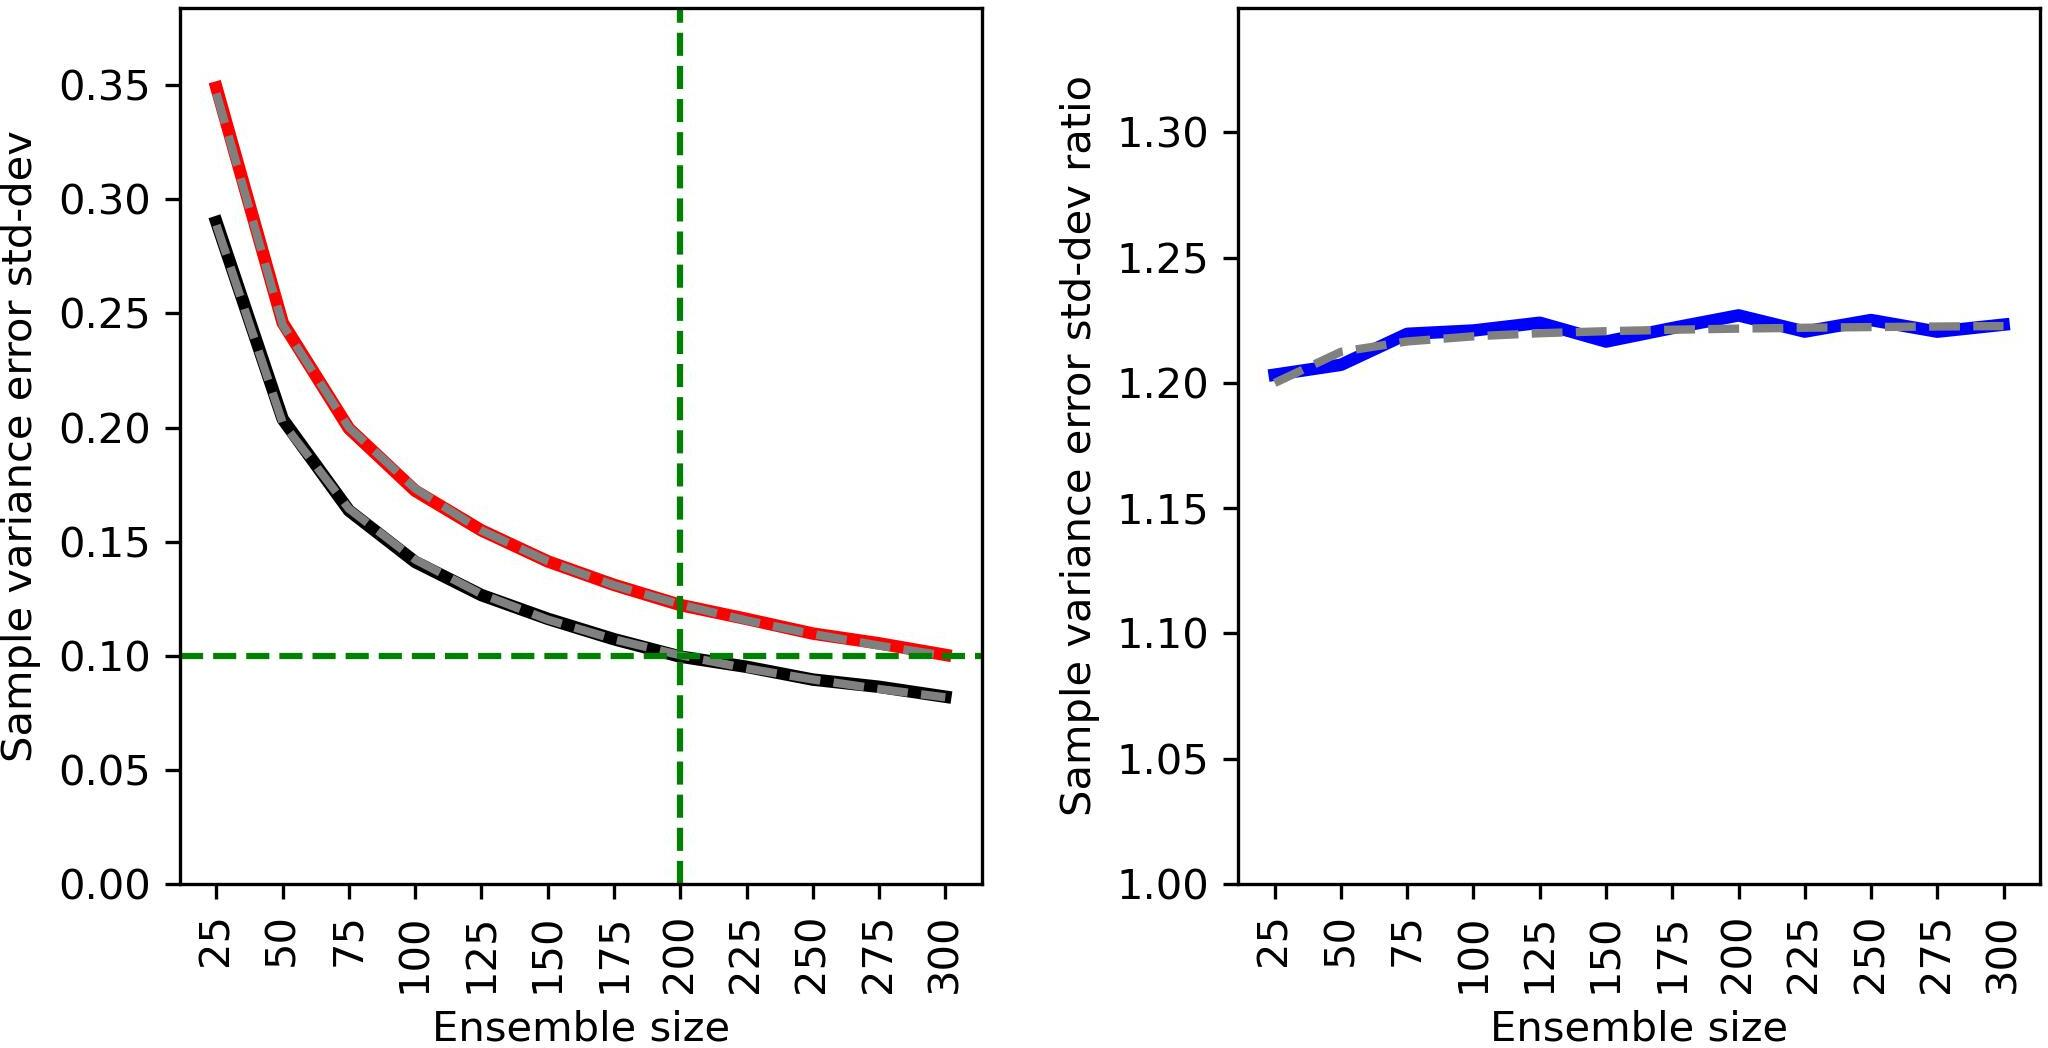
\includegraphics[width=\textwidth]{theory_1.0.jpg}
  \caption{Left: sample variance error standard deviation, black: standard estimator, red: circular estimator, gray dashed: respective theoretical values. Right: ratio of standard-deviation, blue: empirical, gray dashed: theoretical value.} \label{fig:theory_1.0}
\end{figure}

\begin{figure}[h!]
  \noindent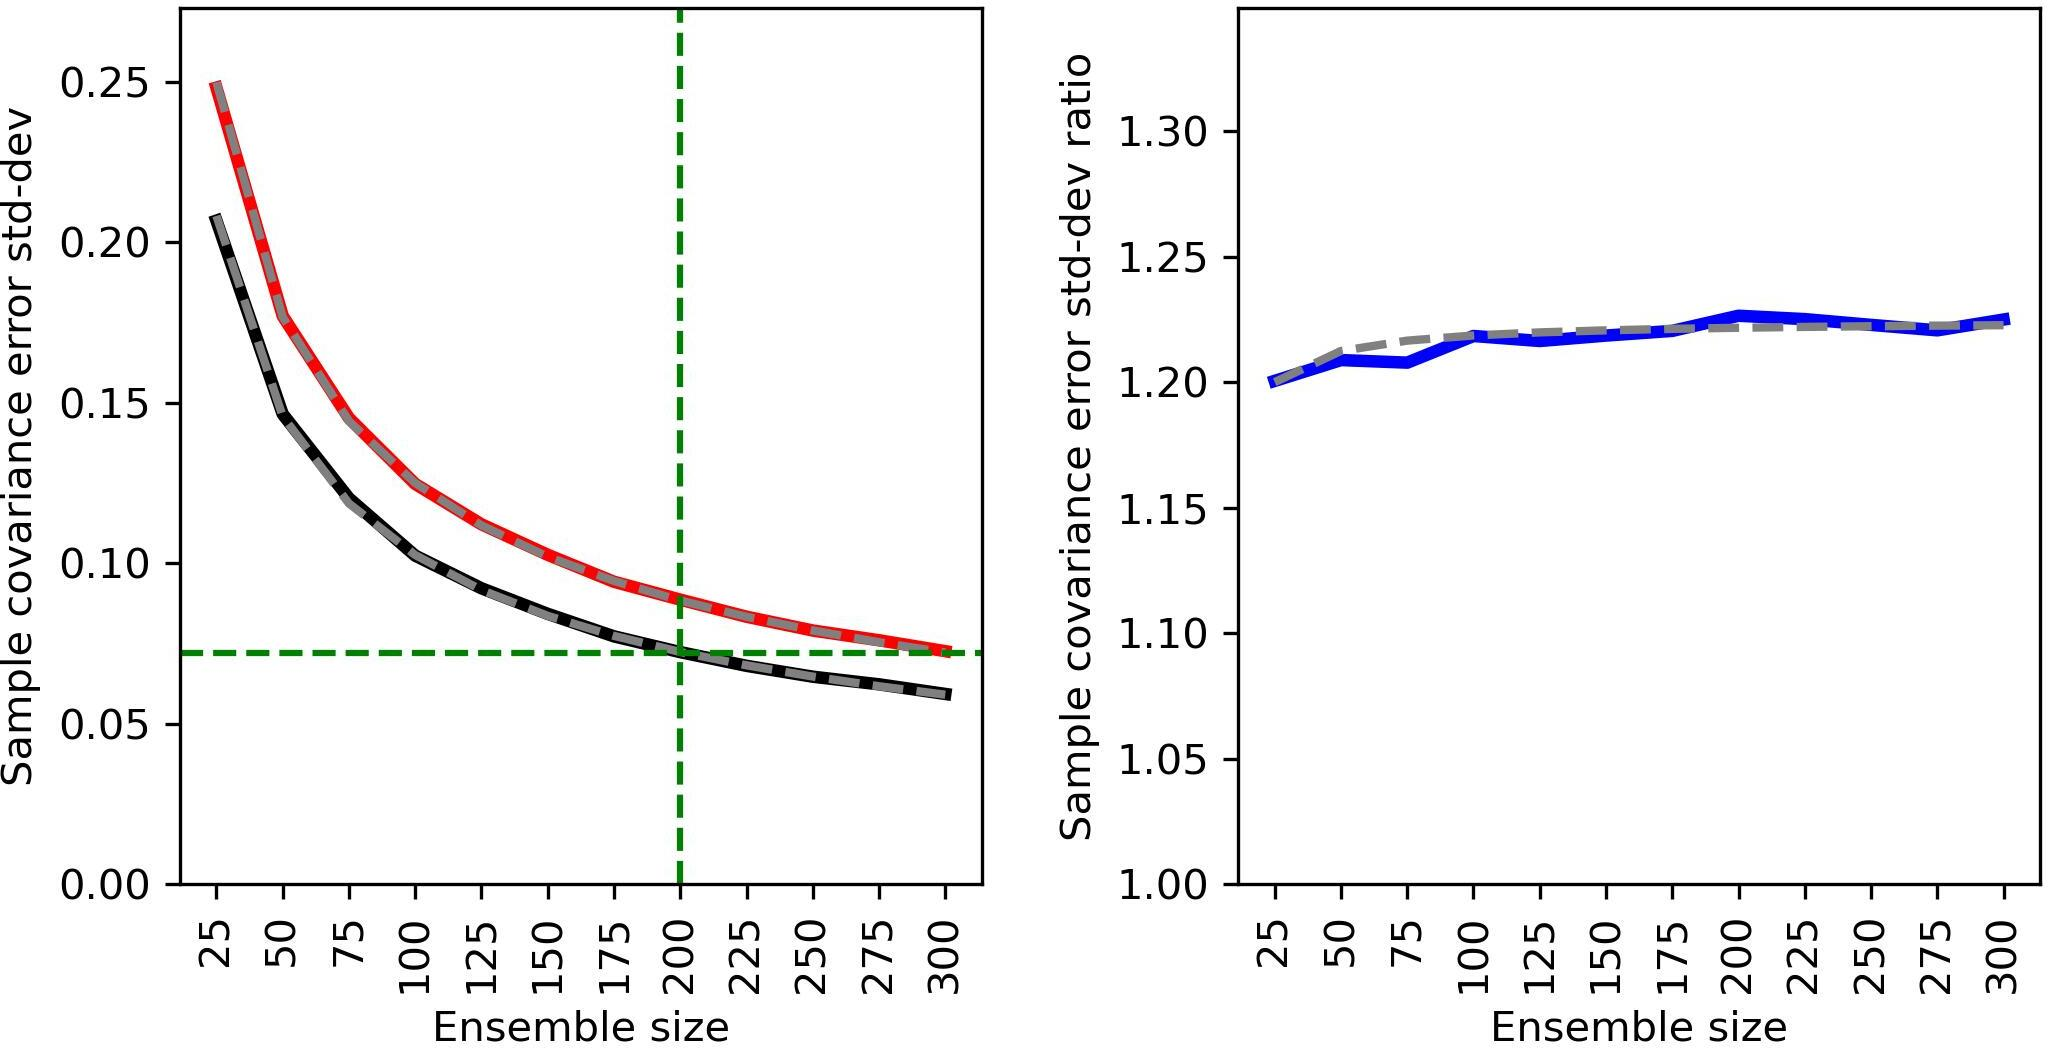
\includegraphics[width=\textwidth]{theory_0.2.jpg}
  \caption{Same as figure \ref{fig:theory_1.0} for the covariance.} \label{fig:theory_0.2}
\end{figure}

\clearpage

\section{Multiple sub-ensembles with distinct distributions}

\subsection{Sub-ensembles characteristics}
Instead of having an ensemble of size $N$ that samples the distribution of a random vector $\mathbf{x}^b$, we assume in this section that we have $R$ ensembles of respective sizes $N_1,\dots,N_R$, with $\sum_{r=1}^R N_r = N$, which sample distinct random vectors $\mathbf{x}^b_1,\dots,\mathbf{x}^b_R$. Each random vector $\mathbf{x}^b_r$ has a distribution characterized by its covariance $\mathbf{B}_r \in \mathbb{R}^{n \times n}$ and its fourth order centered moment $\boldsymbol{\Xi}_r \in \mathbb{R}^{n \times n \times n \times n}$. For each sub-ensemble $\left\{\widetilde{\mathbf{x}}^b_{r,1},\dots,\widetilde{\mathbf{x}}^b_{r,N_r}\right\}$, we define the centered counterparts:
\begin{align}
\delta \widetilde{\mathbf{x}}^b_{r,p} = \widetilde{\mathbf{x}}^b_{r,p} - \langle \widetilde{\mathbf{x}}^b _r\rangle
\end{align}
where $\langle \cdot \rangle$ denotes the sub-ensemble mean:
\begin{align}
\langle \widetilde{\mathbf{x}}^b_r \rangle = \frac{1}{N_r} \sum_{p=1}^{N_r} \widetilde{\mathbf{x}}^b_{r,p}
\end{align}
For each sub-ensemble, centered moments can be estimated from these perturbations by:
\begin{subequations}
\begin{align}
\widetilde{B}_{ij,r} & = \frac{1}{N_r-1} \sum_{p=1}^{N_r} \delta \widetilde{x}^b_{i,r,p} \delta \widetilde{x}^b_{j,r,p}  \\
\widetilde{\Xi}_{ijkl,r} & = \frac{1}{N_r} \sum_{p=1}^{N_r} \delta \widetilde{x}^b_{i,r,p} \delta \widetilde{x}^b_{j,r,p} \delta \widetilde{x}^b_{k,r,p} \delta \widetilde{x}^b_{l,r,p}
\end{align}
\end{subequations}
$  $\\
If the sub-ensemble size $N_r$ goes to infinity, asymptotic $\widetilde{\mathbf{B}}_r$ and $\widetilde{\boldsymbol{\Xi}}_r$ converge to $\mathbf{B}_r$ and $\boldsymbol{\Xi}_r$ respectively:
\begin{subequations}
\begin{align}
\lim_{N_r \rightarrow \infty} \widetilde{\mathbf{B}}_r & = \mathbf{B}_r \\
\lim_{N_r \rightarrow \infty} \widetilde{\boldsymbol{\Xi}}_r & = \boldsymbol{\Xi}_r
\end{align}
\end{subequations}

\subsection{Full ensemble sample covariance issues}
If we consider the full ensemble $\left\{\widetilde{\mathbf{x}}_{1,1},\dots,\widetilde{\mathbf{x}}_{1,N_1},\dots, \widetilde{\mathbf{x}}_{R,1},\dots,\widetilde{\mathbf{x}}_{R,N_R}\right\}$, its ensemble mean is:
\begin{align}
\langle \widetilde{\mathbf{x}} \rangle = \frac{1}{N} \sum_{r=1}^R \sum_{p_r=1}^{N_r} \widetilde{\mathbf{x}}_{r,p_r}
\end{align}
which can be expressed as:
\begin{align}
\langle \widetilde{\mathbf{x}} \rangle & = \frac{1}{N} \sum_{s=1}^R N_s \langle \widetilde{\mathbf{x}}_s \rangle \nonumber \\
 & = \langle \widetilde{\mathbf{x}}_r \rangle + \sum_{s=1}^R \frac{N_s}{N} \left(\langle \widetilde{\mathbf{x}}_s \rangle - \langle \widetilde{\mathbf{x}}_r \rangle \right)
\end{align}
The sample covariance matrix of the full ensemble is given by:
\begin{align}
\label{eq:cov_estim_full}
\widetilde{B}^F_{ij} & = \frac{1}{N-1} \sum_{r=1}^R \sum_{p_r=1}^{N_r} \left(\widetilde{x}_{i,r,p_r} - \langle \widetilde{x}_{i} \rangle\right) \left(\widetilde{x}_{j,r,p_r} - \langle \widetilde{x}_{j} \rangle\right)
\end{align}
Using the expansion of the full ensemble mean, we get for each sub-ensemble $r$:
\begin{align}
& \sum_{p_r=1}^{N_r} \left(\widetilde{x}_{i,r,p_r} - \langle \widetilde{x}_{i} \rangle\right) \left(\widetilde{x}_{j,r,p_r} - \langle \widetilde{x}_{j} \rangle\right) \nonumber \\
= \ & \sum_{p_r=1}^{N_r} \left(\widetilde{x}_{i,r,p_r} - \langle \widetilde{x}_{i,r} \rangle - \sum_{s=1}^R \frac{N_s}{N} \left(\langle \widetilde{x}_{i,s} \rangle - \langle \widetilde{x}_{i,r} \rangle \right) \right)  \left(\widetilde{x}_{j,r,p_r} - \langle \widetilde{x}_{j,r} \rangle - \sum_{t=1}^R \frac{N_t}{N} \left(\langle \widetilde{x}_{j,t} \rangle - \langle \widetilde{x}_{j,r} \rangle \right) \right) \nonumber \\
= \ & \sum_{p_r=1}^{N_r} \left(\widetilde{x}_{i,r,p_r} - \langle \widetilde{x}_{i,r} \rangle \right) \left(\widetilde{x}_{j,r,p_r} - \langle \widetilde{x}_{j,r} \rangle \right) + \sum_{p_r=1}^{N_r} \sum_{1 \le s,t \le R} \frac{N_s N_t}{N^2} \left(\langle \widetilde{x}_{i,s} \rangle - \langle \widetilde{x}_{i,r} \rangle \right) \left(\langle \widetilde{x}_{j,t} \rangle - \langle \widetilde{x}_{j,r} \rangle \right) \nonumber \\
= \ & \left(N_r-1\right) \widetilde{B}_{ij,r} + \sum_{1 \le s,t \le R} \frac{N_r N_s N_t}{N^2} \left(\langle \widetilde{x}_{i,s} \rangle - \langle \widetilde{x}_{i,r} \rangle \right) \left(\langle \widetilde{x}_{j,t} \rangle - \langle \widetilde{x}_{j,r} \rangle \right)
\end{align}
Using the same process as for equation \eqref{eq:cov_estim_2}, the last term summed over all the sub-ensembles becomes:
\begin{align}
& \sum_{1 \le r,s,t \le R} \frac{N_r N_s N_t}{N^2} \left(\langle \widetilde{x}_{i,s} \rangle - \langle \widetilde{x}_{i,r} \rangle \right) \left(\langle \widetilde{x}_{j,t} \rangle - \langle \widetilde{x}_{j,r} \rangle \right) \nonumber \\
= \ & \sum_{1 \le r < s \le R} \frac{N_r N_s}{R N^2} \left(\langle \widetilde{x}_{i,s} \rangle - \langle \widetilde{x}_{i,r} \rangle \right) \left(\langle \widetilde{x}_{j,s} \rangle - \langle \widetilde{x}_{j,r} \rangle \right)
\end{align}
Thus, the sample covariance matrix of equation for the full ensemble can be expressed as:
\begin{align}
\widetilde{B}^F_{ij} =  \frac{1}{N-1} \left(\sum_{r=1}^R \left(N_r-1\right) \widetilde{B}_{ij,r} + \sum_{1 \le r < s \le R} \frac{N_r N_s}{R N^2} \left(\langle \widetilde{x}_{i,s} \rangle - \langle \widetilde{x}_{i,r} \rangle \right) \left(\langle \widetilde{x}_{j,s} \rangle - \langle \widetilde{x}_{j,r} \rangle \right) \right)
\end{align}
It appears that the full ensemble sample covariance $\widetilde{\mathbf{B}}^F$ is not a linear combination of the sub-ensemble sample covariances. Indeed, there is also a term involving products of sub-ensemble means if these sample means differ between sub-ensembles.\\
$  $\\
The expectation of a sub-ensemble mean is simply the distribution mean:
\begin{align}
\mathbb{E} \left[\langle \widetilde{x}_{i,r} \rangle \right] = \mathbb{E} \left[x_{i,r} \right]
\end{align}
Moreover, the covariance of two elements $i$ and $j$ of a same sub-ensemble mean is given equation \eqref{eq:cov_means}:
\begin{align}
\Cov \left[\langle \widetilde{x}_{i,r} \rangle,\langle \widetilde{x}_{j,r} \rangle \right] = \frac{1}{N_r} B_{ij,r}
\end{align}
whereas for distinct sub-ensembles $r \ne s$:
\begin{align}
\Cov \left[\langle \widetilde{x}_{i,r} \rangle,\langle \widetilde{x}_{j,s} \rangle \right] = 0
\end{align}
Using the classical formula for covariances, we get:
\begin{align}
\mathbb{E} \left[\langle \widetilde{x}_{i,r} \rangle \langle \widetilde{x}_{j,r} \rangle\right] & = \Cov \left[\langle \widetilde{x}_{i,r} \rangle,\langle \widetilde{x}_{j,r} \rangle \right] + \mathbb{E} \left[\langle \widetilde{x}_{i,r} \rangle \right] \mathbb{E} \left[ \langle \widetilde{x}_{j,r} \rangle\right] \nonumber \\
& = \frac{1}{N_r} B_{ij,r} + \mathbb{E} \left[x_{i,r} \right] \mathbb{E} \left[x_{j,r} \right]
\end{align}
and for distinct sub-ensembles $r \ne s$:
\begin{align}
\mathbb{E} \left[\langle \widetilde{x}_{i,r} \rangle \langle \widetilde{x}_{j,s} \rangle\right] = \mathbb{E} \left[x_{i,r}\right] \mathbb{E} \left[x_{j,s}\right]
\end{align}
With these results, we can compute the expectation of the full ensemble sample covariance matrix:
\begin{align}
\mathbb{E} \left[\widetilde{B}^F_{ij}\right] & = \frac{1}{N-1} \left(\sum_{r=1}^R \left(N_r-1\right) B_{ij,r} + \sum_{1 \le r < s \le R} \frac{N_r N_s}{R N^2} \left(\frac{1}{N_r} B_{ij,r} + \frac{1}{N_s} B_{ij,s} \right. \right.\nonumber \\
& \left. \left. \quad + \mathbb{E} \left[x_{i,r} \right] \mathbb{E} \left[x_{j,r} \right] + \mathbb{E} \left[x_{i,s} \right] \mathbb{E} \left[x_{j,s} \right] - \mathbb{E} \left[x_{i,r}\right] \mathbb{E} \left[x_{j,s}\right] - \mathbb{E} \left[x_{i,s}\right] \mathbb{E} \left[x_{j,r}\right] \right) \right) \nonumber \\
& = \frac{1}{N-1} \left(\sum_{r=1}^R \left(N_r-1\right) B_{ij,r} + \frac{1}{R N^2} \sum_{1 \le r < s \le R} \left(N_s B_{ij,r} + N_r B_{ij,s}\right) \right. \nonumber \\
& \left. \quad + \sum_{1 \le r < s \le R} \frac{N_r N_s}{R N^2} \left(\mathbb{E} \left[x_{i,s} \right] - \mathbb{E} \left[x_{i,r} \right]\right)\left(\mathbb{E} \left[x_{j,s} \right] - \mathbb{E} \left[x_{j,r} \right] \right)\right)
\end{align}
This equation is a confirmation of the systematic impact of distributions means differences on the full ensemble expected sample covariance $\widetilde{\mathbf{B}}^F$, which is not a desired property.

\subsection{Corrected sample moments}
As a solution, we can remove sub-ensemble means for each sub-ensemble in the calculation of the full ensemble sample covariance. We define the sum of perturbations products $\widetilde{\mathbf{S}}^c$:
\begin{align}
\widetilde{S}^c_{ij} & = \sum_{r=1}^R \sum_{p_r=1}^{N_r} \left(\widetilde{x}_{i,r,p_r} - \langle \widetilde{x}_{i,r} \rangle\right) \left(\widetilde{x}_{j,r,p_r} - \langle \widetilde{x}_{j,r} \rangle\right) \nonumber \\
& = \sum_{r=1}^R \left(N_r-1\right) \widetilde{B}_{ij,r}
\end{align}
Its expectation is given by:
\begin{align}
\mathbb{E} \left[\widetilde{S}^c_{ij}\right] = \sum_{r=1}^R \left(N_r-1\right) B_{ij,r}
\end{align}
and we look for a corrected sample covariance matrix $\widetilde{\mathbf{B}}^c$ that would be proportional to $\widetilde{\mathbf{S}}^c$, with a proportionality coefficient $\alpha$ such that if $\mathbf{B}_1 = \dots = \mathbf{B}_R = \mathbf{B}$, then $\mathbb{E} \left[\widetilde{\mathbf{B}}^c\right] = \mathbf{B}$. Since:
\begin{align}
\mathbb{E} \left[\widetilde{B}^c_{ij}\right] & = \alpha \mathbb{E} \left[\widetilde{S}^c_{ij}\right] \nonumber \\
& = \alpha \sum_{r=1}^R \left(N_r-1\right) B_{ij} \nonumber \\
& = \alpha (N-R) B_{ij}
\end{align}
then $\alpha = (N-R)^{-1}$ and:
\begin{align}
\widetilde{B}^c_{ij} & = \frac{1}{N-R} \widetilde{S}^c_{ij}
\end{align}
This is consistent with the fact that the ensemble of $N$ perturbations where $R$ sub-ensemble means have been removed have only $N-R$ degrees of freedom left.\\
$  $\\
Similarly, for the sample fourth-order centered moment, we define the sum of perturbations products $\widetilde{\boldsymbol{\Psi}}^c$:
\begin{align}
\widetilde{\Psi}^c_{ijkl} & = \sum_{r=1}^R \sum_{p_r=1}^{N_r} \left(\widetilde{x}_{i,r,p_r} - \langle \widetilde{x}_{i,r} \rangle\right) \left(\widetilde{x}_{j,r,p_r} - \langle \widetilde{x}_{j,r} \rangle\right) \left(\widetilde{x}_{k,r,p_r} - \langle \widetilde{x}_{k,r} \rangle\right) \left(\widetilde{x}_{l,r,p_r} - \langle \widetilde{x}_{l,r} \rangle\right) \nonumber \\
& = \sum_{r=1}^R N_r \widetilde{\Xi}_{ijkl,r}
\end{align}
Since the sample fourth-order centered moment estimator is biased, the previous method cannot be applied to find an appropriate normalization. Thus, we choose an arbitrary (but consistent) one for the corrected sample fourth-order centered moment:
\begin{align}
\widetilde{\Xi}^c_{ijkl} = \frac{1}{N} \widetilde{\Psi}^c_{ijkl}
\end{align}

\subsection{Asymptotic behavior}
The corrected sample covariance $\widetilde{\mathbf{B}}^c$ is a linear combination of sub-ensemble sample covariances, the weights being related to the relative sizes of sub-ensembles. If we define $\boldsymbol{\gamma} \in [0,1]^R$ such that $N_r = \gamma_r N$, then we get:
\begin{align}
\widetilde{B}^c_{ij} & = \sum_{r=1}^R \frac{\gamma_r N-1}{N-R} \widetilde{B}_{ij,r}
\end{align}
We denote $\mathbf{B}^c$ the asymptotic limit of $\widetilde{\mathbf{B}}^c$ while $\boldsymbol{\gamma}$ remains constant:
\begin{align}
B^c_{ij} = \lim_{N \rightarrow \infty} \widetilde{B}^c_{ij} = \sum_{r=1}^R \gamma_r B_{ij,r}
\end{align}
The expected corrected sample covariance is:
\begin{align}
\mathbb{E} \left[\widetilde{B}^c_{ij}\right] =  \sum_{r=1}^R \frac{\gamma_r N-1}{N-R} B_{ij,r}
\end{align}
so if $\gamma_r \ne (\gamma_r N-1)/(N-R)$, asymptotic and expected corrected sample covariances are not equal:
\begin{align}
B^c_{ij} \ne \mathbb{E} \left[\widetilde{B}^c_{ij}\right]
\end{align}
$  $\\
The corrected sample fourth-order centered moment $\widetilde{\boldsymbol{\Xi}}^c$ is also a linear combination of sub-ensembles sample fourth-order centered moments, with weigths $\gamma_r = N_r/N$:
\begin{align}
\widetilde{\Xi}^c_{ijkl} & = \sum_{r=1}^R \gamma_r \widetilde{\Xi}_{ijkl,r}
\end{align}
We denote $\boldsymbol{\Xi}^c$ the asymptotic limit of $\widetilde{\boldsymbol{\Xi}}^c$ while $\boldsymbol{\gamma}$ remains constant:
\begin{align}
\Xi^c_{ijkl} = \lim_{N \rightarrow \infty} \widetilde{\Xi}^c_{ijkl} = \sum_{r=1}^R \gamma_r \Xi_{ijkl,r}
\end{align}
The expected corrected sample fourth-order centered moment is:
\begin{align}
\mathbb{E} \left[\widetilde{\Xi}^c_{ijkl}\right] & = \sum_{r=1}^R \gamma_r \mathbb{E} \left[\widetilde{\Xi}_{ijkl,r}\right] \nonumber \\
& = \sum_{r=1}^R \gamma_r \left(P_5(N_r) \ \Xi_{ijkl,r} + P_6(N_r) \left(B_{ij,r}B_{kl,r} + B_{ik,r}B_{jl,r} + B_{il,r}B_{jk,r} \right)\right)
\end{align}

\subsection{Case of equal sub-ensemble sizes}
In the case where all sub-ensemble sizes are equal ($N_1 = \dots = N_R = N/R$), then $\gamma_r = 1/R$ and:
\begin{align}
\frac{\gamma_r N-1}{N-R} = \frac{N/R-1}{N-R} = \frac{1}{R}
\end{align}
so that the corrected sample covariance $\widetilde{\mathbf{B}}^c$ becomes the regular average of sub-ensemble sample covariances:
\begin{align}
\label{eq:Bc}
\widetilde{B}^c_{ij} = \frac{1}{R} \sum_{r=1}^R \widetilde{B}_{ij,r}
\end{align}
As a consequence, the asymptotic and expected corrected sample covariances are equal:
\begin{align}
B^c_{ij} = \frac{1}{R} \sum_{r=1}^R B_{ij,r} = \mathbb{E} \left[\widetilde{B}^c_{ij}\right]
\end{align}
The corrected sample fourth-order centered moment $\widetilde{\boldsymbol{\Xi}}^c$ becomes also the regular average of sub-ensemble sample fourth-order centered moment:
\begin{align}
\label{eq:Xic}
\widetilde{\Xi}^c_{ijkl} = \frac{1}{R} \sum_{r=1}^R \widetilde{\Xi}_{ijkl,r}
\end{align}

\clearpage

\section{Iterative estimation of centered moments}

\subsection{General case}
The mean of an ensemble of $N$ members $\left\{\widetilde{\mathbf{x}}^b_1,\dots,\widetilde{\mathbf{x}}^b_N\right\}$ is computed by:
\begin{align}
\left\langle \widetilde{x}^b_i \right\rangle_N = \frac{1}{N} \sum_{p=1}^N \widetilde{x}^b_{i,p}
\end{align}
where the index $N$ indicates the size of the ensemble over which the mean is computed. This equation can be transformed into:
\begin{align}
\label{eq:moy_rec}
\left\langle \widetilde{x}^b_i \right\rangle_N & = \frac{1}{N} \left(\widetilde{x}^b_{i,N} + \sum_{p=1}^{N-1} \widetilde{x}^b_{i,p} \right) \nonumber \\
 & = \frac{1}{N} \left(\widetilde{x}^b_{i,N} + (N-1) \left\langle \widetilde{x}^b_i \right\rangle_{N-1} \right) \nonumber \\
 & = \left\langle \widetilde{x}^b_i \right\rangle_{N-1} + \frac{1}{N} \left(\widetilde{x}^b_{i,N} - \left\langle \widetilde{x}^b_i \right\rangle_{N-1}\right)
\end{align}
From this formula, $\left\langle \widetilde{x}^b_i \right\rangle_N$ can be updated knowing $\left\langle \widetilde{x}^b_i \right\rangle_{N-1}$ and a new member $\widetilde{x}^b_{i,N}$.
$  $\\
Similarly, the sum $s_{\mathbf{k},N}$ where $\mathbf{k} \in \mathbb{N}^n$ is defined as:
\begin{align}
s_{\mathbf{k},N} = \sum_{p=1}^N \prod_{i=1}^n \left(\widetilde{x}^b_{i,p} - \left\langle \widetilde{x}^b_i \right\rangle_N\right)^{k_i}
\end{align}
This sum can be split in two terms:
\begin{align}
\label{eq:sep}
s_{\mathbf{k},N} = \sum_{p=1}^{N-1} \prod_{i=1}^n \left(\widetilde{x}^b_{i,p} - \left\langle \widetilde{x}^b_i \right\rangle_N\right)^{k_i}  + \prod_{i=1}^n \left(\widetilde{x}^b_{i,N} - \left\langle \widetilde{x}^b_i \right\rangle_N\right)^{k_i}
\end{align}
Using equation \eqref{eq:moy_rec} for the recursive computation of the mean and the binomial theorem, the first term of equation \eqref{eq:sep} can be expanded in:
\begin{align}
&   \sum_{p=1}^{N-1} \prod_{i=1}^n \left(\widetilde{x}^b_{i,p} - \left\langle \widetilde{x}^b_i \right\rangle_N\right)^{k_i} \nonumber \\
& = \sum_{p=1}^{N-1} \prod_{i=1}^n \left(\widetilde{x}^b_{i,p} - \left\langle \widetilde{x}^b_i \right\rangle_{N-1} - \frac{1}{N} \left(\widetilde{x}^b_{i,N} - \left\langle \widetilde{x}^b_i \right\rangle_{N-1}\right)\right)^{k_i} \nonumber \\
& = \sum_{p=1}^{N-1} \prod_{i=1}^n \sum_{m_i=0}^{k_i} \binom{k_i}{m_i} \left(\widetilde{x}^b_{i,p} - \left\langle \widetilde{x}^b_i \right\rangle_{N-1}\right)^{m_i}\left(-\frac{1}{N} \left(\widetilde{x}^b_{i,N} - \left\langle \widetilde{x}^b_i \right\rangle_{N-1}\right)\right)^{k_i-m_i}
\end{align}
where $\mathbf{m} \in \mathbb{N}^n$. Rearranging the sums to extract $p$-dependent factors, we get:
\begin{align}
&   \sum_{p=1}^{N-1} \prod_{i=1}^n \left(\widetilde{x}^b_{i,p} - \left\langle \widetilde{x}^b_i \right\rangle_N\right)^{k_i} \nonumber \\
& = \sum_{p=1}^{N-1} \sum_{m_1=0}^{k_1} \dots \sum_{m_n=0}^{k_n} \prod_{i=1}^n \left(\binom{k_i}{m_i} \left(\frac{-1}{N}\right)^{k_i-m_i} \left(\widetilde{x}^b_{i,p} - \left\langle \widetilde{x}^b_i \right\rangle_{N-1}\right)^{m_i} \right. \nonumber \\
& \quad \times  \left. \left(\widetilde{x}^b_{i,N} - \left\langle \widetilde{x}^b_i \right\rangle_{N-1}\right)^{k_i-m_i} \right) \nonumber \\
& = \sum_{m_1=0}^{k_1} \dots \sum_{m_n=0}^{k_n} \left(\frac{-1}{N}\right)^{\sum_{i=1}^n (k_i-m_i)} \prod_{i=1}^n \left(\binom{k_i}{m_i} \left(\widetilde{x}^b_{i,N} - \left\langle \widetilde{x}^b_i \right\rangle_{N-1}\right)^{k_i-m_i} \right) \nonumber \\
& \quad \times \sum_{p=1}^{N-1} \prod_{i=1}^n \left(\widetilde{x}^b_{i,p} - \left\langle \widetilde{x}^b_i \right\rangle_{N-1}\right)^{m_i} \nonumber \\
& = \sum_{m_1=0}^{k_1} \dots \sum_{m_n=0}^{k_n} \left(\frac{-1}{N}\right)^{\sum_{i=1}^n (k_i-m_i)} \prod_{i=1}^n \left(\binom{k_i}{m_i} \left(\widetilde{x}^b_{i,N} - \left\langle \widetilde{x}^b_i \right\rangle_{N-1}\right)^{k_i-m_i} \right) s_{\mathbf{m},N-1}
\end{align}
The second term of \eqref{eq:sep} is simply modified in:
\begin{align}
\prod_{i=1}^n \left(\widetilde{x}^b_{i,N} - \left\langle \widetilde{x}^b_i \right\rangle_N\right)^{k_i} & = \prod_{i=1}^n \left(\frac{N-1}{N} \left(\widetilde{x}^b_{i,N} - \left\langle \widetilde{x}^b_i \right\rangle_{N-1}\right)\right)^{k_i} \nonumber \\
& = \left(\frac{N-1}{N}\right)^{\sum_{i=1}^n k_i} \prod_{i=1}^n \left(\widetilde{x}^b_{i,N} - \left\langle \widetilde{x}^b_i \right\rangle_{N-1}\right)^{k_i}
\end{align}
Thus, bringing the two terms together:
\begin{align}
\label{eq:som_rec}
s_{\mathbf{k},N} & = \sum_{m_1=0}^{k_1} \dots \sum_{m_n=0}^{k_n} \left(\frac{-1}{N}\right)^{\sum_{i=1}^n (k_i-m_i)} \prod_{i=1}^n \left(\binom{k_i}{m_i} \left(\widetilde{x}^b_{i,N} - \left\langle \widetilde{x}^b_i \right\rangle_{N-1}\right)^{k_i-m_i} \right) s_{\mathbf{m},N-1} \nonumber \\
& \quad + \left(\frac{N-1}{N}\right)^{\sum_{i=1}^n k_i} \prod_{i=1}^n \left(\widetilde{x}^b_{i,N} - \left\langle \widetilde{x}^b_i \right\rangle_{N-1}\right)^{k_i}
\end{align}

\subsection{Covariance and fourth-order centered moment}
For sake of clarity, we define an operator $/ \dots /$ taking as many integers as necessary as inputs, such as:
\begin{align}
/ ijkl \dots / =
\left\{ \begin{array}{rl}
1 & \text{if indices }i,j,k,l, \dots \text{ are all different} \\
0 & \text{else}
\end{array} \right.
\end{align}
To estimate the fourth-order centered moment, at most four elements of the random vector are involved. To simplify the notations, we can assume that the size of the random vector is only $n=4$, other elements being discarded. The algorithm to compute $\widetilde{\mathbf{B}}$ and $\widetilde{\boldsymbol{\Xi}}$ iteratively is:
\begin{enumerate}
\item Load the first member $\widetilde{\mathbf{x}}^b_1$.
\item Initialize all the variables:
\begin{itemize}
\item $\boldsymbol{\mu} = \widetilde{\mathbf{x}}^b_1$,
\item all the sums $s_{\mathbf{k},1}$ are set to zero.
\end{itemize}
\item For $p$ between 2 and $N$ :
\begin{itemize}
\item Load $p^\text{th}$ member $\widetilde{\mathbf{x}}^b_p$.
\item Update the fourth-order sum, $s_{(1,1,1,1),p}$ :
\begin{align}
s_{(1,1,1,1),p} & = s_{(1,1,1,1),p-1} - \frac{1}{p} \sum_{i=1}^4 \left(\widetilde{x}^b_{i,p} - \langle \widetilde{x}^b_i \rangle_{p-1}\right) s_{(/1i/,/2i/,/3i/,/4i/),p-1} \nonumber \\
& \quad + \frac{1}{p^2} \sum_{1 \le i,j \le 4}  \left(\widetilde{x}^b_{i,p} - \langle \widetilde{x}^b_i \rangle_{p-1}\right) \left(\widetilde{x}^b_{j,p} - \langle \widetilde{x}^b_j \rangle_{p-1}\right) \nonumber \\
& \quad \times s_{(/1ij/,/2ij/,/3ij/,/4ij/),p-1} \nonumber \\
& \quad + \frac{(p-1)(p^2-3p+3)}{p^3} \prod_{i=1}^4 \left(\widetilde{x}^b_{i,p} - \langle \widetilde{x}^b_i \rangle_{p-1}\right)
\end{align}
\item Update third-order sums, of form $s_{\mathbf{k},p}$ where $\mathbf{k}$ is a permutation of the vector $(1,1,1,0)$. For instance with $s_{(1,1,1,0),p}$:
\begin{align}
s_{(1,1,1,0),p} & = s_{(1,1,1,0),p-1} - \frac{1}{p} \sum_{i=1}^3 \left(\widetilde{x}^b_{i,p} - \langle \widetilde{x}^b_i \rangle_{p-1}\right) s_{(/1i/,/2i/,/3i/,0),p-1}  \nonumber \\
& \quad + \frac{(p-1)(p-2)}{p^2} \prod_{i=1}^3 \left(\widetilde{x}^b_{i,p} - \langle \widetilde{x}^b_i \rangle_{p-1}\right)
\end{align}
\item Update second-order sums, of form $s_{\mathbf{k},p}$ where $\mathbf{k}$ is a permutation of the vector $(1,1,0,0)$. For instance with $s_{(1,1,0,0),p}$:
\begin{align}
s_{(1,1,0,0),p} = s_{(1,1,0,0),p-1} + \frac{p-1}{p} \left(\widetilde{x}^b_{1,p} - \langle \widetilde{x}^b_1 \rangle_{p-1}\right) \left(\widetilde{x}^b_{2,p} - \langle \widetilde{x}^b_2 \rangle_{p-1}\right)
\end{align}
\item Update means:
\begin{align}
\boldsymbol{\mu} = \boldsymbol{\mu} + \frac{1}{p} \left(\widetilde{\mathbf{x}}^b_p - \boldsymbol{\mu}\right)
\end{align}
\end{itemize}
\item Normalize sums to get centered moments:
\begin{itemize}
\item Covariances:
\begin{align}
\widetilde{B}_{12} = \frac{1}{N-1} s_{(1,1,0,0),N}
\end{align}
\item Fourth-order centered moments:
\begin{align}
\widetilde{\Xi}_{1234} = \frac{1}{N} s_{(1,1,1,1),N}
\end{align}
\end{itemize}
\end{enumerate}

\clearpage

\part{Filtering sample covariances}

\section{Use of the sampling theory}

\subsection{Random processes modeling}
In linear filtering theory, the ``truth'' $\mathbf{B}$ is considered as a random variable, from which we have a noisy estimation $\widetilde{\mathbf{B}}$ only \citep{wiener_1949}. It should be noted that in the previous section, the truth was considered as a fixed and known value, which is not the case anymore.\\
$  $\\
We model the generation of sample centered moments $\widetilde{\mathbf{B}}$ and $\widetilde{\boldsymbol{\Xi}}$ as a two-step random process:
\begin{enumerate}
\item First, a random process $\mathcal{R}$ generates the asymptotic centered moments $\mathbf{B}$ and $\boldsymbol{\Xi}$.
\item Second, a random process $\widetilde{\mathcal{R}}$ generates the sample $\left\{\widetilde{\mathbf{x}}^b_1,\dots,\widetilde{\mathbf{x}}^b_N\right\}$, whose statistical properties are consistent with the realization of $\mathbf{B}$ and $\boldsymbol{\Xi}$ obtained after the first random process $\mathcal{R}$. The sample centered moments $\widetilde{\mathbf{B}}$ and $\widetilde{\boldsymbol{\Xi}}$ are then estimated from this sample.
\end{enumerate}
Since they have very different natures, it seems reasonable to assume that these random processes are independent:
\begin{align}
\label{eq:inde_process}
\mathcal{R} \independent \widetilde{\mathcal{R}}
\end{align}
It is possible to take both processes into account in the sample centered moments statistics. Hereafter, the expectation symbol $\mathbb{E}\left[\cdot\right]$ thus applies to both processes together. In particular, equations \eqref{eq:exp_cov}, \eqref{eq:exp_prod} and \eqref{eq:exp_mom_4} becomes respectively:
\begin{align}
\label{eq:exp_cov_exp}
\mathbb{E} \left[\widetilde{B}_{ij}\right] = \mathbb{E} \left[B_{ij}\right]
\end{align}
\begin{align}
\label{eq:exp_prod_exp}
\mathbb{E} \left[\widetilde{B}_{ij} \widetilde{B}_{kl}\right] & = P_1(N) \ \mathbb{E} \left[\Xi_{ijkl}\right] + P_2(N) \ \mathbb{E} \left[B_{ij} B_{kl}\right] \nonumber \\
& \quad + P_3(N) \left(\mathbb{E} \left[B_{ik} B_{jl}\right] + \mathbb{E} \left[B_{il} B_{jk}\right]\right)
\end{align}
and
\begin{align}
\label{eq:exp_mom_4_exp}
\mathbb{E} \left[\widetilde{\Xi}_{ijkl}\right] = P_5(N) \ \mathbb{E} \left[\Xi_{ijkl}\right]+ P_6(N) \left(\mathbb{E} \left[B_{ij}B_{kl}\right] + \mathbb{E} \left[B_{ik}B_{jl}\right] + \mathbb{E} \left[B_{il}B_{jk}\right] \right)
\end{align}
$  $\\
In the case of a Gaussian distributed ensemble, equation \eqref{eq:exp_prod_gau} becomes:
\begin{align}
\label{eq:exp_prod_gau_exp}
\mathbb{E} \left[\widetilde{B}_{ij} \widetilde{B}_{kl}\right] = \mathbb{E} \left[B_{ij} B_{kl}\right] + P_4(N) \left(\mathbb{E} \left[B_{ik} B_{jl}\right] + \mathbb{E} \left[B_{il} B_{jk}\right]\right)
\end{align}
$  $\\
As another consequence of the independence \eqref{eq:inde_process}, the expected product of an asymptotic sample covariance and a covariance sampling error vanishes:
\begin{align}
& \mathbb{E}\left[\widetilde{B}^e_{ij} B_{kl} \right] = 0 \\
\label{eq:truth_noise_inde}
\Leftrightarrow \ & \mathbb{E}\left[\widetilde{B}_{ij} B_{kl} \right] = \mathbb{E}\left[B_{ij} B_{kl} \right]
\end{align}

\subsection{Linear relations between expected raw and asymptotic quantities}
Noticing that the indices permutations of the sample fourth-order centered moment are all equal: $\widetilde{\Xi}_{ijkl} = \widetilde{\Xi}_{ikjl} = \widetilde{\Xi}_{iljk}$, indices permutations of equation \eqref{eq:exp_prod_exp} and equation \eqref{eq:exp_mom_4_exp} lead to a linear system $\mathbf{A}_N \mathbf{x} = \widetilde{\mathbf{x}}$ with:
\begin{align}
\mathbf{A}_N = \left( \begin{array}{cccc}
P_2(N) & P_3(N) & P_3(N) & P_1(N) \\
P_3(N) & P_2(N) & P_3(N) & P_1(N) \\
P_3(N) & P_3(N) & P_2(N) & P_1(N) \\
P_6(N) & P_6(N) & P_6(N) & P_5(N)
\end{array} \right) , \
\mathbf{x} = \left( \begin{array}{c}
\mathbb{E} \left[B_{ij} B_{kl}\right] \\
\mathbb{E} \left[B_{ik} B_{jl}\right] \\
\mathbb{E} \left[B_{il} B_{jk}\right] \\
\mathbb{E} \left[\Xi_{ijkl}\right]
\end{array} \right) \text{ and }
\widetilde{\mathbf{x}} = \left( \begin{array}{c}
\mathbb{E} \left[\widetilde{B}_{ij} \widetilde{B}_{kl}\right] \\
\mathbb{E} \left[\widetilde{B}_{ik} \widetilde{B}_{jl}\right] \\
\mathbb{E} \left[\widetilde{B}_{il} \widetilde{B}_{jk}\right] \\
\mathbb{E} \left[\widetilde{\Xi}_{ijkl}\right]
\end{array} \right) \nonumber
\end{align}
The matrix $\mathbf{A}_N$ can be inverted:
\begin{align}
\label{eq:invert_lin_sys}
\mathbf{A}_N^{-1} = \left( \begin{array}{cccc}
P_8(N) & P_9(N) & P_9(N) & P_{10}(N) \\
P_9(N) & P_8(N) & P_9(N) & P_{10}(N) \\
P_9(N) & P_9(N) & P_8(N) & P_{10}(N) \\
P_{11}(N) & P_{11}(N) & P_{11}(N) & P_{12}(N)
\end{array} \right)
\end{align}
with:
\begin{subequations}
\begin{align}
P_8(N) & = \frac{2 P_1(N) P_6(N) - P_5(N)\left(P_2(N)+P_3(N)\right)}{\left(P_2(N)-P_3(N)\right)\left(3 P_1(N) P_6(N) - P_5(N) \left(P_2(N) + 2P_3(N)\right)\right)} \nonumber \\
& = \frac{(N-1)(N^2-3N+1)}{N(N-2)(N-3)} \\
P_9(N) & = \frac{P_3(N) P_5(N) - P_1(N) P_6(N)}{\left(P_2(N)-P_3(N)\right)\left(3 P_1(N) P_6(N) - P_5(N) \left(P_2(N) + 2 P_3(N)\right)\right)} \nonumber \\
& = \frac{N-1}{N(N-2)(N-3)} \\
P_{10}(N) & = \frac{P_1(N)}{\left(3 P_1(N) P_6(N) - P_5(N) \left(P_2(N) + 2P_3(N)\right)\right)} \nonumber \\
& = -\frac{N}{(N-2)(N-3)} \\
P_{11}(N) & = \frac{P_6(N)}{\left(3 P_1(N) P_6(N) - P_5(N) \left(P_2(N) + 2P_3(N)\right)\right)} \nonumber \\
& = -\frac{(N-1)(2N-3)}{N(N-2)(N-3)} \\
P_{12}(N) & = -\frac{P_2(N)+2 P_3(N)}{\left(3 P_1(N) P_6(N) - P_5(N) \left(P_2(N) + 2P_3(N)\right)\right)} \nonumber \\
& = \frac{N(N^2-2N+3)}{(N-1)(N-2)(N-3)}
\end{align}
\end{subequations}
to get $\mathbf{x} = \mathbf{A}_N^{-1} \widetilde{\mathbf{x}}$, which is equivalent to:
\begin{subequations}
\begin{align}
\label{eq:prod_asy_cov}
\mathbb{E} \left[B_{ij} B_{kl}\right] & = P_8(N) \ \mathbb{E} \left[\widetilde{B}_{ij} \widetilde{B}_{kl}\right] + P_9(N) \left(\mathbb{E} \left[\widetilde{B}_{ik} \widetilde{B}_{jl}\right] + \mathbb{E} \left[\widetilde{B}_{il} \widetilde{B}_{jk}\right]\right) \nonumber \\
& \quad + P_{10}(N) \ \mathbb{E} \left[\widetilde{\Xi}_{ijkl}\right] \\
\label{eq:asy_mom_4}
\mathbb{E} \left[\Xi_{ijkl}\right] & = P_{11}(N) \ \left(\mathbb{E} \left[\widetilde{B}_{ij} \widetilde{B}_{kl}\right] + \mathbb{E} \left[\widetilde{B}_{ik} \widetilde{B}_{jl}\right] + \mathbb{E} \left[\widetilde{B}_{il} \widetilde{B}_{jk}\right]\right) + P_{12}(N) \ \mathbb{E} \left[\widetilde{\Xi}_{ijkl}\right]
\end{align}
\end{subequations}
$  $\\
In the case of a Gaussian distributed ensemble, the expected product of covariances \eqref{eq:exp_prod_gau_exp} and its indices permutations lead to a linear system $\mathbf{A}_N \mathbf{x} = \widetilde{\mathbf{x}}$ with:
\begin{align}
\mathbf{A}_N & = \left( \begin{array}{ccc}
1 & P_4(N) & P_4(N) \\
P_4(N) & 1 & P_4(N) \\
P_4(N) & P_4(N) & 1 \\
\end{array} \right) , \
\mathbf{x} & = \left( \begin{array}{c}
\mathbb{E} \left[B_{ij} B_{kl}\right] \\
\mathbb{E} \left[B_{ik} B_{jl}\right] \\
\mathbb{E} \left[B_{il} B_{jk}\right]
\end{array} \right) \text{ and }
\widetilde{\mathbf{x}} & = \left( \begin{array}{c}
\mathbb{E} \left[\widetilde{B}_{ij} \widetilde{B}_{kl}\right] \\
\mathbb{E} \left[\widetilde{B}_{ik} \widetilde{B}_{jl}\right] \\
\mathbb{E} \left[\widetilde{B}_{il} \widetilde{B}_{jk}\right]
\end{array} \right) \nonumber
\end{align}
The matrix $\mathbf{A}_N$ can be inverted:
\begin{align}
\label{eq:invert_lin_sys_gau}
\mathbf{A}_N^{-1} = \left( \begin{array}{ccc}
P_{13}(N) & P_{14}(N) & P_{14}(N) \\
P_{14}(N) & P_{13}(N) & P_{14}(N) \\
P_{14}(N) & P_{14}(N) & P_{13}(N)
\end{array} \right)
\end{align}
with:
\begin{subequations}
\begin{align}
P_{13}(N) & = \frac{1 + P_4(N)}{\left(1 - P_4(N)\right)\left(1 + 2P_4(N)\right)} = \frac{N(N-1)}{(N-2)(N+1)} \\
P_{14}(N) & = \frac{-P_4(N)}{\left(1 - P_4(N)\right)\left(1 + 2P_4(N)\right)} = -\frac{N-1}{(N-2)(N+1)}
\end{align}
\end{subequations}
to get $\mathbf{x} = \mathbf{A}_N^{-1} \widetilde{\mathbf{x}}$, which is equivalent to:
\begin{align}
\label{eq:prod_asy_cov_gau}
\mathbb{E} \left[B_{ij} B_{kl}\right] = P_{13}(N) \ \mathbb{E} \left[\widetilde{B}_{ij} \widetilde{B}_{kl}\right] + P_{14}(N) \left(\mathbb{E} \left[\widetilde{B}_{ik} \widetilde{B}_{jl}\right] + \mathbb{E} \left[\widetilde{B}_{il} \widetilde{B}_{jk}\right]\right)
\end{align}

\subsection{Particular case}
For the rest of this document, we only deal with the subcase where $k=i$ and $l=j$.\\
$ $\\
Denoting $\widetilde{\boldsymbol{\xi}} \in \mathbb{R}^{n \times n}$ the matrix such that $\widetilde{\xi}_{ij} = \widetilde{\Xi}_{ijij}$, equations \eqref{eq:exp_prod_exp} and \eqref{eq:exp_mom_4_exp} become:
\begin{subequations}
\begin{align}
\label{eq:exp_prod_exp_2}
\mathbb{E} \left[\widetilde{B}_{ij}^2\right] & = P_1(N) \mathbb{E} \left[\xi_{ij}\right] + P_7(N) \mathbb{E} \left[B^2_{ij}\right] + P_3(N) \mathbb{E} \left[B_{ii} B_{jj}\right] \\
\label{eq:exp_prod_exp_3}
\mathbb{E} \left[\widetilde{B}_{ii} \widetilde{B}_{jj}\right] & = P_1(N) \mathbb{E} \left[\xi_{ij}\right] + 2 P_3(N) \mathbb{E} \left[B^2_{ij}\right] + P_2(N) \mathbb{E} \left[B_{ii} B_{jj}\right] \\
\label{eq:exp_mom_4_exp_2}
\mathbb{E} \left[\widetilde{\xi}_{ij}\right] & = P_5(N) \mathbb{E} \left[\xi_{ij} \right] + P_6(N) \left(2 \mathbb{E} \left[B^2_{ij}\right] + \mathbb{E} \left[B_{ii} B_{jj}\right] \right)
\end{align}
\end{subequations}
with:
\begin{align}
P_7(N) = P_2(N) + P_3(N) =  \frac{N^2-2N+2}{N(N-1)}
\end{align}
Reciprocally, equations \eqref{eq:prod_asy_cov} and \eqref{eq:asy_mom_4} becomes:
\begin{subequations}
\begin{align}
\label{eq:prod_asy_cov_exp_2}
\mathbb{E} \left[B^2_{ij}\right] & = P_{15}(N) \mathbb{E} \left[\widetilde{B}^2_{ij}\right] + P_9(N) \mathbb{E} \left[\widetilde{B}_{ii} \widetilde{B}_{jj}\right] + P_{10}(N) \mathbb{E} \left[\widetilde{\xi}_{ij}\right] \\
\label{eq:prod_asy_cov_exp_3}
\mathbb{E} \left[B_{ii} B_{jj}\right] & = 2P_9(N) \mathbb{E} \left[\widetilde{B}^2_{ij}\right] + P_8(N) \mathbb{E} \left[\widetilde{B}_{ii} \widetilde{B}_{jj}\right] + P_{10}(N) \mathbb{E} \left[\widetilde{\xi}_{ij}\right] \\
\label{eq:asy_mom_4_exp_2}
\mathbb{E} \left[\xi_{ij}\right] & = P_{11}(N) \left(2 \mathbb{E} \left[\widetilde{B}_{ij}^2\right] + \mathbb{E} \left[\widetilde{B}_{ii} \widetilde{B}_{jj}\right] \right) + P_{12}(N) \ \mathbb{E} \left[\widetilde{\xi}_{ij}\right]
\end{align}
\end{subequations}
with:
\begin{align}
P_{15}(N) = P_8(N) + P_9(N) =  \frac{(N-1)^2}{N(N-3)}
\end{align}
$  $\\
In the case of a Gaussian distributed ensemble, equation \eqref{eq:exp_prod_gau_exp} is used instead:
\begin{subequations}
\begin{align}
\label{eq:exp_prod_gau_exp_2}
\mathbb{E} \left[\widetilde{B}_{ij}^2\right] & = P_{16}(N) \mathbb{E} \left[B^2_{ij}\right] + P_4(N) \mathbb{E} \left[B_{ii} B_{jj}\right] \\
\label{eq:exp_prod_gau_exp_3}
\mathbb{E} \left[\widetilde{B}_{ii} \widetilde{B}_{jj}\right] & = 2 P_4(N) \mathbb{E} \left[B^2_{ij}\right] + \mathbb{E} \left[B_{ii} B_{jj}\right]
\end{align}
\end{subequations}
with:
\begin{align}
P_{16}(N) = 1 + P_4(N) = \frac{N}{N-1}
\end{align}
Reciprocally, equation \eqref{eq:prod_asy_cov_gau} becomes:
\begin{subequations}
\begin{align}
\label{eq:prod_asy_cov_gau_exp_2}
\mathbb{E} \left[B^2_{ij}\right] & = P_{17}(N) \mathbb{E} \left[ \widetilde{B}_{ij}^2 \right] + P_{14}(N) \mathbb{E} \left[\widetilde{B}_{ii} \widetilde{B}_{jj} \right] \\
\label{eq:prod_asy_cov_gau_exp_3}
\mathbb{E} \left[B_{ii} B_{jj}\right] & = 2 P_{14}(N) \mathbb{E} \left[\widetilde{B}_{ij}^2\right] + P_{13}(N) \mathbb{E} \left[\widetilde{B}_{ii} \widetilde{B}_{jj}\right]
\end{align}
\end{subequations}
with:
\begin{align}
P_{17}(N) = P_{13}(N) + P_{14}(N) = \frac{(N-1)^2}{(N-2)(N+1)}
\end{align}

\subsection{Diagnostics for any ensemble size}
Expected ensemble quantities can be estimated from an ensemble of size $N$, allowing the estimation of expected asymptotic quantities. Interestingly, these quantities can be used to estimate expected raw quantities for an hypothetic ensemble with the same distribution but of a different size $N'$.\\
$  $\\
\tikzset{box/.style={draw,inner sep=2mm,outer sep=0mm,align=center,thin,fill=white}}
\begin{center}
\begin{tikzpicture}[auto,>=latex]
    \node[box] (exp) {\begin{tabular}{@{\hspace{0.07cm}}c@{\hspace{0.07cm}}}
                                     Expected ensemble quantities  \\
                                     from a given ensemble (size $N$): \\
                                     $\mathbb{E} \left[\widetilde{B}_{ij}\right]$, $\mathbb{E} \left[\widetilde{B}_{ij}^2\right]$, $\mathbb{E} \left[\widetilde{B}_{ii} \widetilde{B}_{jj}\right]$, $\mathbb{E} \left[\widetilde{\xi}_{ij}\right]$
                                      \end{tabular}};

    \node[box, below of=exp, node distance=2.0cm, xshift=8.0cm] (asy) {\begin{tabular}{@{\hspace{0.07cm}}c@{\hspace{0.07cm}}}
                                     Expected asymptotic quantities: \\
                                     from this distribution: \\
                                     $\mathbb{E} \left[B_{ij}\right]$, $\mathbb{E} \left[B^2_{ij}\right]$, $\mathbb{E} \left[B_{ii} B_{jj}\right]$, $\mathbb{E} \left[\xi_{ij}\right]$
                                      \end{tabular}};

    \node[box, below of=exp, node distance=4.0cm] (exp2) {\begin{tabular}{@{\hspace{0.07cm}}c@{\hspace{0.07cm}}}
                                     Expected ensemble quantities  \\
                                     from this distribution (size $N'$): \\
                                     $\mathbb{E} \left[\widetilde{B}_{ij}\right]$, $\mathbb{E} \left[\widetilde{B}_{ij}^2\right]$, $\mathbb{E} \left[\widetilde{B}_{ii} \widetilde{B}_{jj}\right]$, $\mathbb{E} \left[\widetilde{\xi}_{ij}\right]$
                                      \end{tabular}};

    \path[->,thick] (exp.east) edge node {\begin{tabular}{@{\hspace{0.07cm}}c@{\hspace{0.07cm}}}
                                     Equations \eqref{eq:exp_cov_exp} and [\eqref{eq:prod_asy_cov_exp_2}, \eqref{eq:prod_asy_cov_exp_3}, \eqref{eq:asy_mom_4_exp_2}] \\
                                     or [\eqref{eq:prod_asy_cov_gau_exp_2}, \eqref{eq:prod_asy_cov_gau_exp_3}] with ensemble size $N$
                                     \end{tabular}} (asy.north);

    \path[->,thick] (asy.south) edge node {\begin{tabular}{@{\hspace{0.07cm}}c@{\hspace{0.07cm}}}
                                     Equations \eqref{eq:exp_cov_exp} and [\eqref{eq:exp_prod_exp_2}, \eqref{eq:exp_prod_exp_3}, \eqref{eq:exp_mom_4_exp_2}] \\
                                     or [\eqref{eq:exp_prod_gau_exp_2}, \eqref{eq:exp_prod_gau_exp_3}] with ensemble size $N'$
                                     \end{tabular}} (exp2.east);
\end{tikzpicture}
\end{center}


\subsection{Multiple sub-ensembles with distinct distributions}
The computation of diagnostics for any ensemble size (previous section) need to be adapted in the framework of multiple sub-ensembles. For sake of simplicity, we consider the case of $R$ sub-ensembles of equal sizes $N_r = N/R$ and we separate the procedure into two steps:
\begin{enumerate}
\item Starting from estimations of $\widetilde{\mathbf{B}}_r$ and $\widetilde{\boldsymbol{\xi}}_r$ for each sub-ensemble, we get from equations \eqref{eq:Bc} and \eqref{eq:Xic}:
\begin{subequations}
\begin{align}
\mathbb{E} \left[\widetilde{B}^c_{ij}\right] & = \frac{1}{R} \sum_{r=1}^R \mathbb{E} \left[\widetilde{B}_{ij,r}\right] \\
\mathbb{E} \left[\widetilde{B}^{c2}_{ij}\right] & = \frac{1}{R^2} \sum_{1 \le r,s \le R} \mathbb{E} \left[\widetilde{B}_{ij,r} \widetilde{B}_{ij,s}\right] \\
\mathbb{E} \left[\widetilde{B}^c_{ii} \widetilde{B}^c_{jj}\right] & = \frac{1}{R^2} \sum_{1 \le r,s \le R} \mathbb{E} \left[\widetilde{B}_{ii,r} \widetilde{B}_{jj,s}\right] \\
\mathbb{E} \left[\widetilde{\xi}_{ij}\right] & = \frac{1}{R} \sum_{r=1}^R \mathbb{E} \left[\widetilde{\xi}_{ij,r}\right]
\end{align}
\end{subequations}

\item From this sampled quantities, we need to estimate asymptotic quantities. First equation is easy:
\begin{align}
\mathbb{E} \left[B^c_{ij}\right] & = \mathbb{E} \left[\widetilde{B}^c_{ij}\right]
\end{align}
Using the independence \eqref{eq:inde_process}, the expected product of aymptotic and sample covariances can be expressed as:
\begin{align}
\mathbb{E} \left[B^c_{ij} \widetilde{B}^c_{kl} \right] & = \frac{1}{R^2} \sum_{1 \le r,s \le R} \mathbb{E} \left[B_{ij,r} \widetilde{B}_{kl,s}\right] \nonumber \\
& = \frac{1}{R^2} \left(\sum_{r=1}^R \mathbb{E} \left[B_{ij,r} B_{kl,r}\right] + \sum_{\substack{1 \le r,s \le R\\r \ne s}} \mathbb{E} \left[B_{ij,r} \widetilde{B}_{kl,s}\right]\right)
\end{align}
The first term can be computed using equation \eqref{eq:prod_asy_cov} for each sub-ensemble. However, an additional assumption is required to estimate the second term. A possible one is to assume that:
\begin{enumerate}
\item the sampling error $\widetilde{B}_{ij,r} - B_{ij,r}$ of sub-ensemble $r$ is not correlated with the sampling error $\widetilde{B}_{kl,s} - B_{kl,s}$ of sub-ensemble $s$:
\begin{align}
\mathbb{E} \left[\left(\widetilde{B}_{ij,r} - B_{ij,r}\right)\left(\widetilde{B}_{kl,s} - B_{kl,s}\right)\right] \approx \mathbb{E} \left[\widetilde{B}_{ij,r} - B_{ij,r}\right] \mathbb{E} \left[\widetilde{B}_{kl,s} - B_{kl,s}\right] = 0
\end{align}
\item the sampling error $\widetilde{B}_{ij,r} - B_{ij,r}$ of sub-ensemble $r$ is not correlated with the asymptotic covariance matrix $B_{kl,s}$ of sub-ensemble $s$:
\begin{align}
\mathbb{E} \left[\left(\widetilde{B}_{ij,r} - B_{ij,r}\right)B_{kl,s}\right] \approx \mathbb{E} \left[\widetilde{B}_{ij,r} - B_{ij,r}\right] \mathbb{E} \left[B_{kl,s}\right] = 0
\end{align}
\end{enumerate}
Thus, we obtain two interesting properties:
\begin{enumerate}
\item $\mathbb{E} \left[B_{ij,r} \widetilde{B}_{kl,s}\right] \approx \mathbb{E} \left[B_{ij,r} B_{kl,s}\right]$, so that $\mathbb{E} \left[B^c_{ij} \widetilde{B}^c_{kl} \right] \approx \mathbb{E} \left[B^c_{ij} B^c_{kl} \right]$, similar to equation \eqref{eq:truth_noise_inde},
\item $\mathbb{E} \left[B_{ij,r} \widetilde{B}_{kl,s}\right] \approx \mathbb{E} \left[\widetilde{B}_{ij,r} \widetilde{B}_{kl,s}\right]$, useful to estimate:
\begin{align}
\mathbb{E} \left[B^c_{ij} \widetilde{B}^c_{kl} \right] = \frac{1}{R^2} \left(\sum_{r=1}^R \mathbb{E} \left[B_{ij,r} B_{kl,r}\right] + \sum_{\substack{1 \le r,s \le R\\r \ne s}} \mathbb{E} \left[\widetilde{B}_{ij,r} \widetilde{B}_{kl,s}\right]\right)
\end{align}
\end{enumerate}
As a consequence, we get the second and third equations:
\begin{subequations}
\begin{align}
\mathbb{E} \left[B^{c2}_{ij} \right] & = \frac{1}{R^2} \left(\sum_{r=1}^R \mathbb{E} \left[B^2_{ij,r}\right] + \sum_{\substack{1 \le r,s \le R\\r \ne s}} \mathbb{E} \left[\widetilde{B}_{ij,r} \widetilde{B}_{ij,s}\right]\right) \\
\mathbb{E} \left[B^c_{ii} B^c_{jj} \right] & = \frac{1}{R^2} \left(\sum_{r=1}^R \mathbb{E} \left[B_{ii,r} B_{jj,r}\right] + \sum_{\substack{1 \le r,s \le R\\r \ne s}} \mathbb{E} \left[\widetilde{B}_{ii,r} \widetilde{B}_{jj,s}\right]\right)
\end{align}
\end{subequations}
where $\mathbb{E} \left[B^2_{ij,r}\right]$ and $\mathbb{E} \left[B_{ii,r} B_{jj,r}\right]$ are computed using equations [\eqref{eq:prod_asy_cov_exp_2}, \eqref{eq:prod_asy_cov_exp_3}] or [\eqref{eq:prod_asy_cov_gau_exp_2}, \eqref{eq:prod_asy_cov_gau_exp_3}] for each sub-ensemble. The last equation is simply:
\begin{align}
\mathbb{E} \left[\xi^c_{ij}\right] & = \frac{1}{R} \sum_{r=1}^R \mathbb{E} \left[\xi_{ij,r}\right]
\end{align}
where $\mathbb{E} \left[\xi_{ij,r}\right]$ is computed using equation \eqref{eq:asy_mom_4_exp_2} for each sub-ensemble.
\end{enumerate}

\clearpage

\section{Filtering optimization}

\subsection{Optimization norms}
We define $\widehat{\mathbf{B}}\left(\boldsymbol{\lambda}\right)$ as the filtered estimate of $\widetilde{\mathbf{B}}$, where $\boldsymbol{\lambda} \in \mathbb{R}^M$ is a vector of parameters and $\widehat{\mathbf{B}}\left(\boldsymbol{\lambda}\right)$ is a linear function of $\boldsymbol{\lambda}$.\\
$  $\\
To optimize $\boldsymbol{\lambda}$, we need to define a norm that should be minimized. A general choice is to use the expected squared Frobenius norm of the filtering error, projected into a subspace defined by the projection matrix $\mathbf{Q} \in \mathbb{R}^{n \times n'}$:
\begin{align}
\label{eq:norm_proj}
e\left(\boldsymbol{\lambda}\right) & = \mathbb{E}\left[ \left\Vert \mathbf{Q}^\mathrm{T} \left(\widehat{\mathbf{B}}\left(\boldsymbol{\lambda}\right) - \mathbf{B} \right) \mathbf{Q} \right\Vert_\mathrm{F}^2 \right]
\end{align}
The asymptotic sample covariance $\mathbf{B}$ can be considered as the target of the filtering. The definition of the projection matrix $\mathbf{Q}$ depends on the considered system.\\
$  $\\
Hereafter, we will focus on a particular case where $\mathbf{Q}$ is square ($n' = n$) and diagonal, leading to:
\begin{align}
\label{eq:norm_proj_2}
e\left(\boldsymbol{\lambda}\right) & = \mathbb{E}\left[ \left\Vert \mathbf{W} \circ \left(\widehat{\mathbf{B}}\left(\boldsymbol{\lambda}\right) - \mathbf{B} \right) \right\Vert_\mathrm{F}^2 \right] \nonumber \\
& = \mathbb{E}\left[ \sum_{1 \le i,j \le n} \left(W_{ij} \left(\widehat{B}_{ij}\left(\boldsymbol{\lambda}\right) - B_{ij} \right) \right)^2 \right] \nonumber \\
& = \sum_{1 \le i,j \le n} W^2_{ij} \mathbb{E}\left[\left(\widehat{B}_{ij}\left(\boldsymbol{\lambda}\right) - B_{ij} \right)^2\right]
\end{align}
where $W_{ij} = Q_{ii} Q_{jj}$ defines a weight matrix applied via a Schur product (element-by-element) denoted $\circ$. The definition of the $\mathbf{W}$ is an open question, but $\mathbf{W}$ should not depend on the ensemble since it is extracted from the expectation $\mathbb{E}\left[\cdot\right]$.

\subsection{Linear filtering optimization}
The gradient of $e\left(\boldsymbol{\lambda}\right)$ with respect to $\lambda_m$ is given by:
\begin{align}
\label{eq:grad}
\frac{\partial e}{\partial \lambda_m} = 2 \sum_{1 \le i,j \le n} W_{ij}^2 \mathbb{E}\left[ \left(\widehat{B}_{ij}\left(\boldsymbol{\lambda}\right) - B_{ij} \right) \frac{\partial \widehat{B}_{ij}}{\partial \lambda_m} \right]
\end{align}
$  $\\
We can define the subset $\mathcal{S}^\mathrm{opt} \subset \mathbf{R}^M$ of the vectors $\boldsymbol{\lambda}^\mathrm{opt}$ canceling the gradient \eqref{eq:grad}:
\begin{align}
\label{eq:grad_zero}
\forall m \in [1,M] \ , \ & \left.\frac{\partial e}{\partial \lambda_m}\right|_{\boldsymbol{\lambda}=\boldsymbol{\lambda}^\mathrm{opt}} = 0
\end{align}
Since $\widehat{\mathbf{B}}\left(\boldsymbol{\lambda}\right)$ is a linear function of $\boldsymbol{\lambda}$, $e\left(\boldsymbol{\lambda}\right)$ is a quadratic and nonnegative function of $\boldsymbol{\lambda}$. Thus any vector $\boldsymbol{\lambda}^\mathrm{opt}$ in $\mathcal{S}^\mathrm{opt}$ is minimizing $e\left(\boldsymbol{\lambda}\right)$, and is an equivalently relevant solution for our problem.

\subsection{Norm reduction}
An interesting property of the linear filtering is the possibility to compute the optimal norm reduction. Since the filtering is linear:
\begin{align}
\widehat{B}_{ij}\left(\boldsymbol{\lambda}\right) = \sum_{1 \le m \le M} \frac{\partial \widehat{B}_{ij}}{\partial \lambda_m} \lambda_m
\end{align}
Equations \eqref{eq:grad} and \eqref{eq:grad_zero} can be combined into:
\begin{align}
\forall m \in [1,M] \ , \ \sum_{1 \le i,j \le n} W_{ij}^2 \mathbb{E}\left[ \left(\widehat{B}_{ij}\left(\boldsymbol{\lambda}^\mathrm{opt}\right) - B_{ij} \right) \left.\frac{\partial \widehat{B}_{ij}}{\partial \lambda_m}\right|_{\boldsymbol{\lambda}=\boldsymbol{\lambda}^\mathrm{opt}} \right] = 0
\end{align}
The sum over $[1,M]$ of the previous equation, post-multiplied by $\lambda^\mathrm{opt}_m$, yields:
\begin{align}
\label{eq:filt_red}
& \sum_{1 \le m \le M} \sum_{1 \le i,j \le n} W_{ij}^2 \mathbb{E}\left[ \left(\widehat{B}_{ij}\left(\boldsymbol{\lambda}^\mathrm{opt}\right) - B_{ij} \right) \left.\frac{\partial \widehat{B}_{ij}}{\partial \lambda_m}\right|_{\boldsymbol{\lambda}=\boldsymbol{\lambda}^\mathrm{opt}} \right] \lambda^\mathrm{opt}_m = 0 \nonumber \\
\Leftrightarrow \ & \sum_{1 \le i,j \le n} W_{ij}^2 \mathbb{E}\left[ \left(\widehat{B}_{ij}\left(\boldsymbol{\lambda}^\mathrm{opt}\right) - B_{ij} \right) \sum_{1 \le m \le M} \left.\frac{\partial \widehat{B}_{ij}}{\partial \lambda_m}\right|_{\boldsymbol{\lambda}=\boldsymbol{\lambda}^\mathrm{opt}} \lambda^\mathrm{opt}_m \right] = 0 \nonumber \\
\Leftrightarrow \ & \sum_{1 \le i,j \le n} W_{ij}^2 \mathbb{E}\left[ \left(\widehat{B}_{ij}\left(\boldsymbol{\lambda}^\mathrm{opt}\right) - B_{ij} \right) \widehat{B}_{ij}\left(\boldsymbol{\lambda}^\mathrm{opt}\right) \right] = 0
\end{align}
We define $\boldsymbol{\lambda}^0$ the vector of parameters such as no filtering is applied: $\widehat{\mathbf{B}}\left(\boldsymbol{\lambda}^0\right) = \widetilde{\mathbf{B}}$. Using the previous property, we can derive:
\begin{align}
e\left(\boldsymbol{\lambda}^0\right) & = \sum_{1 \le i,j \le n} W_{ij}^2 \mathbb{E}\left[ \left(\widetilde{B}_{ij} - B_{ij} \right)^2 \right] \nonumber \\
& = \sum_{1 \le i,j \le n} W_{ij}^2 \mathbb{E}\left[ \left(\left(\widehat{B}_{ij}\left(\boldsymbol{\lambda}^\mathrm{opt}\right) - B_{ij}\right) - \left(\widehat{B}_{ij}\left(\boldsymbol{\lambda}^\mathrm{opt}\right) - \widetilde{B}_{ij}\right)\right)^2 \right] \nonumber \\
& = \sum_{1 \le i,j \le n} W_{ij}^2 \mathbb{E}\left[ \left(\widehat{B}_{ij}\left(\boldsymbol{\lambda}^\mathrm{opt}\right) - B_{ij}\right)^2\right] + \sum_{1 \le i,j \le n} W_{ij}^2 \mathbb{E}\left[ \left(\widehat{B}_{ij}\left(\boldsymbol{\lambda}^\mathrm{opt}\right) - \widetilde{B}_{ij}\right)^2\right] \nonumber \\
& \quad - 2 \sum_{1 \le i,j \le n} W_{ij}^2 \mathbb{E}\left[\left(\widehat{B}_{ij}\left(\boldsymbol{\lambda}^\mathrm{opt}\right) - B_{ij}\right) \left(\widehat{B}_{ij}\left(\boldsymbol{\lambda}^\mathrm{opt}\right) - \widetilde{B}_{ij}\right) \right]
\end{align}
Reducing the last term with equation \eqref{eq:filt_red}, we get:
\begin{align}
\label{eq:de}
e\left(\boldsymbol{\lambda}^0\right) - e\left(\boldsymbol{\lambda}^\mathrm{opt}\right) = \Delta e + 2 \sum_{1 \le i,j \le n} W_{ij}^2 \mathbb{E}\left[ \left(\widehat{B}_{ij}\left(\boldsymbol{\lambda}^\mathrm{opt}\right) - B_{ij}\right) \widetilde{B}_{ij} \right]
\end{align}
where:
\begin{align}
\Delta e = \sum_{1 \le i,j \le n} W_{ij}^2 \mathbb{E}\left[ \left(\widehat{B}_{ij}\left(\boldsymbol{\lambda}^\mathrm{opt}\right) - \widetilde{B}_{ij}\right)^2\right]
\end{align}
The difference $e\left(\boldsymbol{\lambda}^0\right) - e\left(\boldsymbol{\lambda}^\mathrm{opt}\right)$ is the norm reduction due to the filtering. If we can show that the last term of equation \eqref{eq:de} vanishes, then $\Delta e$ can be computed once $\widehat{B}_{ij}\left(\boldsymbol{\lambda}^\mathrm{opt}\right)$ is known to estimate this norm reduction. Actually, an even more general condition given by $\displaystyle \mathbb{E}\left[\left(\widehat{B}_{ij}\left(\boldsymbol{\lambda}^\mathrm{opt}\right) - B_{ij}\right) \widetilde{B}_{ij}  \right] = 0$ will be verified in the following filtering methods.\\
$  $\\
Also:
\begin{align}
e\left(\boldsymbol{\lambda}^0\right) & = \sum_{1 \le i,j \le n} W_{ij}^2 \mathbb{E}\left[ \left(\widetilde{B}_{ij} - B_{ij} \right)^2 \right] \nonumber \\
& = \sum_{1 \le i,j \le n} W_{ij}^2 \left(\mathbb{E}\left[ \widetilde{B}_{ij}^2 \right] + \mathbb{E}\left[ B^2_{ij} \right] - 2 \mathbb{E}\left[ \widetilde{B}_{ij} B_{ij} \right] \right) \nonumber \\
& = \sum_{1 \le i,j \le n} W_{ij}^2 \left(\mathbb{E}\left[ \widetilde{B}_{ij}^2 \right] - \mathbb{E}\left[ B^2_{ij} \right]\right)
\end{align}
which can be used to compute a relative norm reduction $\displaystyle \frac{e\left(\boldsymbol{\lambda}^0\right) - e\left(\boldsymbol{\lambda}^\mathrm{opt}\right)}{e\left(\boldsymbol{\lambda}^0\right)}$.

\clearpage

\section{Variance filtering}

\subsection{Filtering method}
Variances are gathered in vectors $\mathbf{v} \in \mathbb{R}^n$:
\begin{subequations}
\begin{align}
v_i & = B_{ii} \\
\widetilde{v}_i & = \widetilde{B}_{ii} \\
\widehat{v}_i & = \widehat{B}_{ii}
\end{align}
\end{subequations}
To filter the sample variances $\widetilde{\mathbf{v}}$, we apply a linear filter (gain and offset). Thus $\widehat{\mathbf{v}}$ is defined as:
\begin{align}
\label{eq:var_filter}
\widehat{\mathbf{v}} = \mathbf{F} \widetilde{\mathbf{v}} + \mathbf{f}
\end{align}
where $\mathbf{F} \in \mathbb{R}^{n \times n}$ is the filtering gain and $\mathbf{f} \in \mathbb{R}^n$ the filter offset.

\subsection{Expected squared norm}
We use the identity matrix as a weight: $\mathbf{W} = \mathbf{I}_n$. The expected squared norm of equation \eqref{eq:norm_proj_2} adapted for the variance filtering becomes:
\begin{align}
e(\mathbf{F},\mathbf{f}) & = \sum_{1 \le i \le n} \mathbb{E}\left[ \left(\sum_{1 \le j \le n} F_{ij} \widetilde{v}_j + f_i - v_i \right)^2 \right] \nonumber \\
& = \sum_{1 \le i \le n} \left( \sum_{1 \le j,k \le n} F_{ij} F_{ik} \mathbb{E}\left[\widetilde{v}_j \widetilde{v}_k\right] + f_i^2 + \mathbb{E}\left[v^2_i\right] \right.\nonumber \\
& \left. \quad + 2 f_i \sum_{1 \le j \le n} F_{ij} \mathbb{E}\left[\widetilde{v}_j\right] - 2 \sum_{1 \le j \le n} F_{ij} \mathbb{E}\left[v_i\widetilde{v}_j\right] - 2 f_i \mathbb{E}\left[v_i\right]\right)
\end{align}
Using the independence of random processes in \eqref{eq:truth_noise_inde}, it can be simplified:
\begin{align}
e(\mathbf{F},\mathbf{f}) & = \sum_{1 \le i \le n} \Bigg( \sum_{1 \le j,k \le n} F_{ij} F_{ik} \mathbb{E}\left[\widetilde{v}_j \widetilde{v}_k\right] + f_i^2 + \mathbb{E}\left[v^2_i\right] \nonumber \\
& + 2 f_i \left(\sum_{1 \le j \le n} F_{ij} \mathbb{E}\left[\widetilde{v}_j\right] - \mathbb{E}\left[\widetilde{v}_i\right]\right)- 2 \sum_{1 \le j \le n} F_{ij} \mathbb{E}\left[v_i v_j\right]\Bigg)
\end{align}
Its gradient is given by:
\begin{subequations}
\begin{align}
\label{eq:var_grad_1}
\frac{\partial e}{\partial F_{ij}} & = 2 \left(\sum_{1 \le k \le n}  F_{ik} \mathbb{E}\left[\widetilde{v}_j \widetilde{v}_k\right] + f_i \mathbb{E}\left[\widetilde{v}_j\right] - \mathbb{E}\left[v_i v_j\right]\right) \\
\frac{\partial e}{\partial f_i} & = 2 \left(f_i + \sum_{1 \le j \le n} F_{ij} \mathbb{E}\left[\widetilde{v}_j\right] - \mathbb{E}\left[\widetilde{v}_i\right]\right)
\end{align}
\end{subequations}

\subsection{Explicit optimality}
Setting the gradient of $e(\mathbf{F},\mathbf{f})$ to zero, we get in a vectorial form:
\begin{align}
\label{eq:var_th_1}
& 2 \left(\mathbf{F}^\mathrm{opt} \mathbb{E}\left[\widetilde{\mathbf{v}} \widetilde{\mathbf{v}}^\mathrm{T}\right] + \mathbf{f}^\mathrm{opt} \mathbb{E}\left[\widetilde{\mathbf{v}}^\mathrm{T}\right] - \mathbb{E}\left[\mathbf{v} \mathbf{v}^\mathrm{T}\right]\right) = 0 \nonumber \\
\Leftrightarrow \ & \mathbf{F}^\mathrm{opt} \mathbb{E}\left[\widetilde{\mathbf{v}} \widetilde{\mathbf{v}}^\mathrm{T}\right] + \mathbf{f}^\mathrm{opt} \mathbb{E}\left[\widetilde{\mathbf{v}}^\mathrm{T}\right] = \mathbb{E}\left[\mathbf{v} \mathbf{v}^\mathrm{T}\right]
\end{align}
and:
\begin{align}
\label{eq:var_th_2}
& 2 \left(\mathbf{F}^\mathrm{opt} \mathbb{E}\left[\widetilde{\mathbf{v}} \right] + \mathbf{f}^\mathrm{opt} - \mathbb{E}\left[\widetilde{\mathbf{v}}\right]\right) = 0 \nonumber \\
\Leftrightarrow \ & \mathbf{F}^\mathrm{opt} \mathbb{E}\left[\widetilde{\mathbf{v}} \right] + \mathbf{f}^\mathrm{opt} = \mathbb{E}\left[\widetilde{\mathbf{v}}\right]
\end{align}
From equation \eqref{eq:var_th_2}, we get the filter offset:
\begin{align}
\mathbf{f}^\mathrm{opt} = \left(\mathbf{I}_n - \mathbf{F}^\mathrm{opt}\right) \mathbb{E}\left[\widetilde{\mathbf{v}}\right]
\end{align}
so that equation \eqref{eq:var_th_1} reads:
\begin{align}
& \mathbf{F}^\mathrm{opt} \mathbb{E}\left[\widetilde{\mathbf{v}} \widetilde{\mathbf{v}}^\mathrm{T}\right] + \left(\mathbf{I}_n - \mathbf{F}^\mathrm{opt}\right) \mathbb{E}\left[\widetilde{\mathbf{v}}\right] \mathbb{E}\left[\widetilde{\mathbf{v}}^\mathrm{T}\right] = \mathbb{E}\left[\mathbf{v} \mathbf{v}^\mathrm{T}\right] \nonumber \\
\Leftrightarrow \ & \mathbf{F}^\mathrm{opt} \left(\mathbb{E}\left[\widetilde{\mathbf{v}} \widetilde{\mathbf{v}}^\mathrm{T}\right] - \mathbb{E}\left[\widetilde{\mathbf{v}}\right] \mathbb{E}\left[\widetilde{\mathbf{v}}^\mathrm{T}\right]\right) = \mathbb{E}\left[\mathbf{v} \mathbf{v}^\mathrm{T}\right] - \mathbb{E}\left[\widetilde{\mathbf{v}}\right] \mathbb{E}\left[\widetilde{\mathbf{v}}^\mathrm{T}\right] \nonumber \\
\Leftrightarrow \ & \mathbf{F}^\mathrm{opt} = \left(\mathbb{E}\left[\mathbf{v} \mathbf{v}^\mathrm{T}\right] - \mathbb{E}\left[\widetilde{\mathbf{v}}\right] \mathbb{E}\left[\widetilde{\mathbf{v}}^\mathrm{T}\right]\right)\left(\mathbb{E}\left[\widetilde{\mathbf{v}} \widetilde{\mathbf{v}}^\mathrm{T}\right] - \mathbb{E}\left[\widetilde{\mathbf{v}}\right] \mathbb{E}\left[\widetilde{\mathbf{v}}^\mathrm{T}\right]\right)^{-1}
\end{align}
Using the independence of random processes in \eqref{eq:truth_noise_inde}, $\mathbb{E}\left[\widetilde{\mathbf{v}}\right] = \mathbb{E}\left[\mathbf{v}\right]$ so that:
\begin{align}
\label{eq:opt_var_filter}
\mathbf{F}^\mathrm{opt} & = \left(\mathbb{E}\left[\mathbf{v} \mathbf{v}^\mathrm{T}\right] - \mathbb{E}\left[\mathbf{v}\right] \mathbb{E}\left[\mathbf{v}^\mathrm{T}\right]\right)\left(\mathbb{E}\left[\widetilde{\mathbf{v}} \widetilde{\mathbf{v}}^\mathrm{T}\right] - \mathbb{E}\left[\widetilde{\mathbf{v}}\right] \mathbb{E}\left[\widetilde{\mathbf{v}}^\mathrm{T}\right]\right)^{-1} \nonumber \\
& = \Cov\left(\mathbf{v}\right) \Cov\left(\widetilde{\mathbf{v}}\right)^{-1}
\end{align}

\subsection{Properties}
Equations \eqref{eq:var_th_1} and \eqref{eq:var_th_2} can be rewritten using the optimally filtered variances $\widehat{\mathbf{v}}^\mathrm{opt} = \mathbf{F}^\mathrm{opt} \widetilde{\mathbf{v}} + \mathbf{f}^\mathrm{opt}$:
\begin{subequations}
\begin{align}
\label{eq:var_flt_1}
\mathbb{E}\left[\widehat{\mathbf{v}}^\mathrm{opt} \widetilde{\mathbf{v}}^\mathrm{T}\right] & = \mathbb{E}\left[\mathbf{v} \mathbf{v}^\mathrm{T}\right] \\
\label{eq:var_flt_2}
\mathbb{E}\left[\widehat{\mathbf{v}}^\mathrm{opt} \right] & = \mathbb{E}\left[\widetilde{\mathbf{v}}\right]
\end{align}
\end{subequations}

\subsection{Norm reduction}
Using the independence of random processes in \eqref{eq:truth_noise_inde} and the optimality condition of equation \eqref{eq:var_flt_1}, we verify that:
\begin{align}
\mathbb{E}\left[\left(\widehat{v}_i^\mathrm{opt} - v_i\right) \widetilde{v}_i \right] = \mathbb{E}\left[\widehat{v}_i^\mathrm{opt} \widetilde{v}_i\right] - \mathbb{E} \left[v_i v_i \right] = 0
\end{align}
so that:
\begin{align}
e\left(\mathbf{I}_n,\boldsymbol{0}\right) - e\left(\mathbf{F}^\mathrm{opt},\mathbf{f}^\mathrm{opt}\right) = \sum_{1 \le i \le n} \mathbb{E}\left[ \left(\widehat{v}_i^\mathrm{opt} - \widetilde{v}_i\right)^2\right]
\end{align}

\clearpage

\section{Localization}

\subsection{Filtering method}
To localize the sample covariances, we apply a localization matrix via a Schur product (element-by-element). Thus $\widehat{\mathbf{B}}$ is defined as:
\begin{align}
\widehat{\mathbf{B}} = \mathbf{L} \circ \widetilde{\mathbf{B}}
\end{align}
where $\mathbf{L} \in \mathbb{R}^{n \times n}$ is the localization matrix.

\subsection{Expected squared norm}
The expected squared norm of equation \eqref{eq:norm_proj_2} adapted for the localization becomes:
\begin{align}
e(\mathbf{L}) & = \sum_{1 \le i,j \le n} W_{ij}^2 \mathbb{E}\left[ \left(L_{ij} \widetilde{B}_{ij} - B_{ij} \right)^2 \right] \nonumber \\
& = \sum_{1 \le i,j \le n} W_{ij}^2 \left(L^2_{ij} \mathbb{E} \left[\widetilde{B}_{ij}^2\right] + \mathbb{E} \left[B^2_{ij}\right] - 2 L_{ij} \mathbb{E} \left[\widetilde{B}_{ij} B_{ij}\right] \right)
\end{align}
Using the independence of random processes in \eqref{eq:truth_noise_inde}, it can be simplified:
\begin{align}
e(\mathbf{L}) & = \sum_{1 \le i,j \le n} W_{ij}^2 \left(L^2_{ij} \mathbb{E} \left[\widetilde{B}_{ij}^2\right] + \left(1 - 2 L_{ij}\right) \mathbb{E} \left[B^2_{ij}\right] \right)
\end{align}
Its gradient is given by:
\begin{align}
\frac{\partial e}{\partial L_{ij}} = 2 W_{ij}^2 \left(L_{ij} \mathbb{E} \left[\widetilde{B}_{ij}^2\right] - \mathbb{E} \left[B^2_{ij}\right] \right)
\end{align}

\subsection{Explicit optimality}
Setting the gradient of $e(\mathbf{L})$ to zero, we get:
\begin{align}
\label{eq:loc_th}
& 2 W_{ij}^2 \left(L^\mathrm{opt}_{ij} \mathbb{E} \left[\widetilde{B}_{ij}^2\right] - \mathbb{E} \left[B^2_{ij}\right]\right) = 0 \ \Leftrightarrow \ L^\mathrm{opt}_{ij} = \frac{\mathbb{E} \left[B^2_{ij}\right]}{\mathbb{E} \left[\widetilde{B}_{ij}^2\right]}
\end{align}
We can notice that the weight matrix $\mathbf{W}$ does not affect $\mathbf{L}^\mathrm{opt}$.

\subsection{Properties}
Using the independence of random processes in \eqref{eq:truth_noise_inde}, we can notice that:
\begin{align}
L^\mathrm{opt}_{ij} = \frac{\mathbb{E}\left[ B^2_{ij} \right]}{\mathbb{E}\left[ \left(B_{ij} + \widetilde{B}^e_{ij}\right)^2 \right]} = \frac{\mathbb{E}\left[ B^2_{ij} \right]}{\mathbb{E}\left[ B^2_{ij} \right] + \mathbb{E}\left[ \widetilde{B}_{ij}^{e2} \right]}
\end{align}
which shows three important properties:
\begin{itemize}
\item The optimal localization is bounded: $0 \le L^\mathrm{opt}_{ij} \le 1$.
\item For a finite ensemble size, sampling noise arises ($\mathbb{E}\left[ \widetilde{B}_{ii}^{e2} \right] > 0$) so that $L^\mathrm{opt}_{ii}$ (at zero separation) is strictly lower than 1, contrary to what can be usually found in the literature.
\item For an infinite ensemble size ($N \rightarrow \infty$), the sampling noise vanishes ($\mathbb{E}\left[ \widetilde{B}_{ij}^{e2} \right] \rightarrow 0$) so that $L^\mathrm{opt}_{ij} \rightarrow 1$: no localization is applied.
\end{itemize}

\subsection{Norm reduction}
Using the independence of random processes in \eqref{eq:truth_noise_inde} and the optimality condition of equation \eqref{eq:loc_th}, we verify that:
\begin{align}
\mathbb{E}\left[\left(\widehat{B}_{ij}^\mathrm{opt} - B_{ij}\right) \widetilde{B}_{ij} \right] = L_{ij}^\mathrm{opt} \mathbb{E}\left[\widetilde{B}_{ij}^2\right] - \mathbb{E}\left[B^2_{ij} \right] = 0
\end{align}
so that:
\begin{align}
e\left(\boldsymbol{1}\right) - e\left(\mathbf{L}^\mathrm{opt}\right) = \sum_{1 \le i,j \le n} W_{ij}^2 \mathbb{E}\left[ \left(\widehat{B}_{ij}^\mathrm{opt} - \widetilde{B}_{ij}\right)^2\right]
\end{align}

\clearpage

\section{Links between localization and correlation}

\subsection{Approximations of the optimal localization}
The sample correlation matrix $\widetilde{\mathbf{C}}$ is defined as:
\begin{align}
\widetilde{C}_{ij} = \frac{\widetilde{B}_{ij}}{\sqrt{\widetilde{B}_{ii} \widetilde{B}_{jj}}}
\end{align}
and the asymptotic limit of $\widetilde{\mathbf{C}}$ is denoted $\mathbf{C}$.\\
$  $\\
In the case of a Gaussian distributed ensemble, we can get two different approximations of the localization:
\begin{enumerate}
\item In a simplified modeling of the asymptotic sample covariance matrix $\mathbf{B}$, we can assume that the asymptotic sample correlation matrix $\mathbf{C}$ is exactly the same at every realization of its generating random process $\mathcal{R}$, with no variability. As a consequence, it can be extracted from expectations:
\begin{align}
\mathbb{E} \left[ B^2_{ij} \right] = \mathbb{E} \left[B_{ii} B_{jj} C^2_{ij} \right] = \mathbb{E} \left[B_{ii} B_{jj} \right] C^2_{ij}
\end{align}
Equation \eqref{eq:exp_prod_gau_exp} gives:
\begin{align}
\mathbb{E} \left[\widetilde{B}_{ij}^2 \right] & = \left(1 + P_4(N)\right) \ \mathbb{E} \left[B^2_{ij}\right] + P_4(N) \ \mathbb{E} \left[B_{ii} B_{jj}\right] \nonumber \\
& = \left(\left(1 + P_4(N)\right) C^2_{ij} + P_4(N) \right) \ \mathbb{E} \left[B_{ii} B_{jj} \right]
\end{align}
so that the optimal localization of equation \eqref{eq:loc_th} is given by:
\begin{align}
\label{eq:local_gau_cor_1}
L^\mathrm{app1}_{ij} & = \frac{\mathbb{E} \left[B^2_{ij}\right]}{\mathbb{E} \left[\widetilde{B}_{ij}^2\right]} \nonumber \\
& = \frac{\mathbb{E} \left[B_{ii} B_{jj} \right] C^2_{ij}}{\left(\left(1 + P_4(N)\right) C^2_{ij} + P_4(N) \right) \ \mathbb{E} \left[B_{ii} B_{jj} \right]} \nonumber \\
& = \frac{C^2_{ij}}{\left(1 + P_4(N)\right) C^2_{ij} + P_4(N)}
\end{align}
if we assume (reasonably) that $\mathbb{E} \left[B_{ii} B_{jj} \right] \ne 0$.
\item A first order approximation of $\mathbb{E} \left[\widetilde{C}_{ij}^2 \right]$ is given by:
\begin{align}
\label{eq:corsq_first_order}
\mathbb{E} \left[\widetilde{C}_{ij}^2 \right] = \mathbb{E} \left[\frac{\widetilde{B}^2_{ij}}{\widetilde{B}_{ii} \widetilde{B}_{jj}} \right] \approx \frac{\mathbb{E} \left[\widetilde{B}_{ij}^2 \right]}{\mathbb{E} \left[\widetilde{B}_{ii} \widetilde{B}_{jj}\right]}
\end{align}
Plugging this result into equation \eqref{eq:prod_asy_cov_gau_exp_2}, we get:
\begin{align}
\mathbb{E} \left[B^2_{ij}\right] \approx P_{17}(N) \ \mathbb{E} \left[\widetilde{B}_{ij}^2\right] + P_{14}(N) \frac{\mathbb{E} \left[\widetilde{B}_{ij}^2\right]}{\mathbb{E} \left[\widetilde{C}_{ij}^2 \right]}
\end{align}
Thus, the optimal localization $\mathbf{L}^\mathrm{opt}$ of equation \eqref{eq:loc_th} can be approximated by:
\begin{align}
\label{eq:local_gau_cor_2}
L^\mathrm{app2}_{ij} = P_{17}(N) + P_{14}(N) \frac{1}{\mathbb{E} \left[\widetilde{C}_{ij}^2\right]}
\end{align}
\end{enumerate}
For a Gaussian distributed ensemble, \citet{rady_2005} proves that:
\begin{align}
\mathbb{E} \left[\widetilde{C}_{ij}^2\right] & = C^2_{ij} \nonumber \\
& \quad + \frac{2 C^4_{ij} - 3 C^2_{ij} + 1}{N-1} \nonumber \\
& \quad + \frac{8 C^6_{ij} - 14 C^4_{ij} + 6 C^2_{ij}}{(N-1)^2} \nonumber \\
& \quad + \frac{48 C^8_{ij} - 104 C^6_{ij} + 68 C^4_{ij} - 12 C^2_{ij}}{(N-1)^3} \nonumber \\
& \quad + O\left(\frac{1}{(N-1)^4}\right)
\end{align}
This result can be used to compare $\mathbf{L}^\mathrm{app1}$ and $\mathbf{L}^\mathrm{app2}$. Figure \ref{fig:corloc} shows that the second approximation gives a more severe localization (for a given asymptotic sample correlation $C_{ij}$, $L^\mathrm{app2}_{ij} \le L^\mathrm{app1}_{ij})$. Interetingly, both approximation seems to converge for $N \rightarrow \infty$.

\begin{center}
\begin{figure}[h!]
  \noindent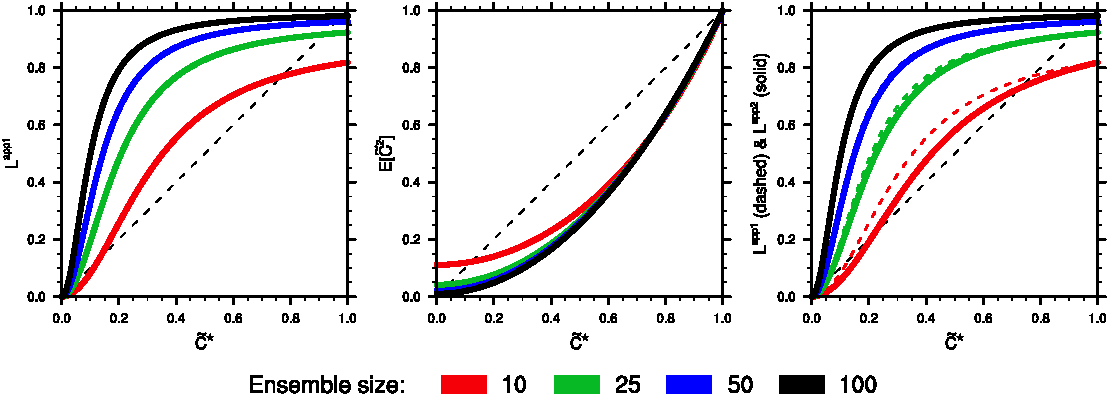
\includegraphics[width=\textwidth]{corloc.pdf}\\
  \caption{} \label{fig:corloc}
\end{figure}
\end{center}

\subsection{Local tensor definition}
The local tensor is a matrix used to define the curvature of a function at its origin. Let $\mathbf{r} = \left(x_1,\dots,x_d\right)^\mathrm{T} \in \mathbb{R}^d$ be a coordinate vector in a $d$-dimensional space. The local correlation tensor $\mathbf{H}^C \in \mathbb{R}^{d \times d}$ associated with the correlation function $C(\mathbf{r})$, assumed to be twice differentiable, is given by:
\begin{align}
\mathbf{H}^C = - \left.\nabla \nabla^\mathrm{T} C\right|_{\mathbf{r}=\mathbf{0}} \ \Leftrightarrow \ H^C_{\alpha,\beta} = - \left.\frac{\partial^2 C}{\partial x_\alpha \partial x_\beta}\right|_{\mathbf{r}=\mathbf{0}}
\end{align}
For a localization function $L(\mathbf{r})$ that is not normalized (i.e. $L(\mathbf{0}) \ne 1$), the local localization tensor definition has to be adapted:
\begin{align}
\mathbf{H}^L = \frac{- \left.\nabla \nabla^\mathrm{T} L\right|_{\mathbf{r}=\mathbf{0}}}{L(\mathbf{0})}\ \Leftrightarrow \ H^L_{\alpha,\beta} = \frac{\displaystyle - \left.\frac{\partial^2 L}{\partial x_\alpha \partial x_\beta}\right|_{\mathbf{r}=\mathbf{0}}}{L(\mathbf{0})}
\end{align}

\subsection{Using the asymptotic sample correlation tensor}
The asymptotic sample correlation $\mathbf{C}$ and the localization $\mathbf{L}^\mathrm{app1}$ are transposed in continuous space and respectively denoted $C(\mathbf{r})$ and $L^\mathrm{app1}(\mathbf{r})$. Equation \eqref{eq:local_gau_cor_2} becomes:
\begin{align}
L^\mathrm{app1} = \frac{C^2}{\left(1 + P_4(N)\right) C^2 + P_4(N)}
\end{align}
The gradient of $L^\mathrm{app1}$ is:
\begin{align}
\frac{\partial L^\mathrm{app1}}{\partial x_\alpha} & = \frac{\displaystyle 2 P_4(N) \ C \frac{\partial C}{\partial x_\alpha}}{\left(\left(1 + P_4(N)\right) C^2 + P_4(N)\right)^2}
\end{align}
and its Hessian matrix is:
\begin{align}
\frac{\partial^2 L^\mathrm{app1}}{\partial x_\alpha \partial x_\beta} & = \frac{\displaystyle 2 P_4(N) \ C \frac{\partial^2 C}{\partial x_\alpha \partial x_\beta}}{\left(\left(1 + P_4(N)\right) C^2 + P_4(N)\right)^2} \nonumber \\
& \quad + \frac{\displaystyle 2 P_4(N) \left(P_4(N) - 3 \left(1 + P_4(N)\right) C^2\right) \frac{\partial C}{\partial x_\alpha} \frac{\partial C}{\partial x_\beta}}{\left(\left(1 + P_4(N)\right) C^2 + P_4(N)\right)^3}
\end{align}
However in $\mathbf{r} = \mathbf{0}$:
\begin{subequations}
\begin{align}
C(\mathbf{0}) & = 1 \\
\left.\frac{\partial C}{\partial x_\alpha}\right|_{\mathbf{r}=\mathbf{0}} & = 0
\end{align}
\end{subequations}
so that:
\begin{align}
\left.\frac{\partial^2 L^\mathrm{app1}}{\partial x_\alpha \partial x_\beta}\right|_{\mathbf{r}=\mathbf{0}} & = \frac{2 P_4(N)}{\left(1 + 2 P_4(N)\right)^2} \left.\frac{\partial^2 C}{\partial x_\alpha \partial x_\beta}\right|_{\mathbf{r}=\mathbf{0}}
\end{align}
Thus, the local localization tensor associated with $L^\mathrm{app1}$ is given by:
\begin{align}
H^{L^\mathrm{app1}}_{\alpha,\beta} & = \frac{\displaystyle - \left.\frac{\partial^2 L^\mathrm{app1}}{\partial x_\alpha \partial x_\beta}\right|_{\mathbf{r}=\mathbf{0}}}{L^\mathrm{app1}(\mathbf{0})} \nonumber \\
& = - \frac{2 P_4(N)}{1 + 2 P_4(N)} \ \left.\frac{\partial^2 C}{\partial x_\alpha \partial x_\beta}\right|_{\mathbf{r}=\mathbf{0}} \nonumber \\
& = P_{18}(N) \ H^{C}_{\alpha,\beta}
\end{align}
with:
\begin{align}
P_{18}(N) = \frac{2 P_4(N)}{1 + 2 P_4(N)} = \frac{2}{N+1}
\end{align}
Since $P_{18}(N)$ is positive, the components of $\mathbf{H}^{L^\mathrm{app1}}$ and $\mathbf{H}^{C}$ have the same sign.

\subsection{Using the squared sample correlation tensor}
The sample correlation $\widetilde{\mathbf{C}}$ and the localization $\mathbf{L}^\mathrm{app2}$ are transposed in continuous space and respectively denoted $\widetilde{C}(\mathbf{r})$ and $L^\mathrm{app2}(\mathbf{r})$. Equation \eqref{eq:local_gau_cor_2} becomes:
\begin{align}
L^\mathrm{app2} = P_{17}(N) + P_{14}(N) \frac{1}{\mathbb{E} \left[\widetilde{C}^2\right]}
\end{align}
The gradient of $L^\mathrm{app2}$ is:
\begin{align}
\frac{\partial L^\mathrm{app2}}{\partial x_\alpha} & = - P_{14}(N) \ \frac{\displaystyle \frac{\partial \mathbb{E} \left[\widetilde{C}^2\right]}{\displaystyle \partial x_\alpha}}{\mathbb{E} \left[\widetilde{C}^2\right]^2}
\end{align}
and its Hessian matrix is:
\begin{align}
\frac{\partial^2 L^\mathrm{app2}}{\partial x_\alpha \partial x_\beta} & = - P_{14}(N) \ \frac{\displaystyle \frac{\partial^2 \mathbb{E} \left[\widetilde{C}^2\right]}{\displaystyle \partial x_\alpha \partial x_\beta} \mathbb{E} \left[\widetilde{C}^2\right] - 2 \frac{\partial \mathbb{E} \left[\widetilde{C}^2\right]}{\displaystyle \partial x_\alpha} \frac{\partial \mathbb{E} \left[\widetilde{C}^2\right]}{\displaystyle \partial x_\beta}}{\mathbb{E} \left[\widetilde{C}^2\right]^3}
\end{align}
However in $\mathbf{r} = \mathbf{0}$:
\begin{subequations}
\begin{align}
\widetilde{C}(\mathbf{0}) & = 1 \\
\left.\frac{\partial \widetilde{C}}{\partial x_\alpha}\right|_{\mathbf{r}=\mathbf{0}} & = 0
\end{align}
\end{subequations}
so that:
\begin{align}
\left.\frac{\partial^2 L^\mathrm{app2}}{\partial x_\alpha \partial x_\beta}\right|_{\mathbf{r}=\mathbf{0}} & = - P_{14}(N) \left.\frac{\partial^2 \mathbb{E} \left[\widetilde{C}^2\right]}{\displaystyle \partial x_\alpha \partial x_\beta} \right|_{\mathbf{r}=\mathbf{0}}
\end{align}
Thus, the local localization tensor associated with $L^\mathrm{app2}$ is given by:
\begin{align}
H^{L^\mathrm{app2}}_{\alpha,\beta} & = \frac{\displaystyle - \left.\frac{\partial^2 L^\mathrm{app2}}{\partial x_\alpha \partial x_\beta}\right|_{\mathbf{r}=\mathbf{0}}}{L^\mathrm{app2}(\mathbf{0})} \nonumber \\
& = \frac{P_{14}(N)}{P_{17}(N) + P_{14}(N)} \left.\frac{\partial^2 \mathbb{E} \left[\widetilde{C}^2\right]}{\displaystyle \partial x_\alpha \partial x_\beta} \right|_{\mathbf{r}=\mathbf{0}} \nonumber \\
& = P_{19}(N) \ H^{\mathbb{E} \left[\widetilde{C}^2\right]}_{\alpha,\beta}
\end{align}
with:
\begin{align}
P_{19}(N) = -\frac{P_{14}(N)}{P_{17}(N) + P_{14}(N)} = \frac{1}{N-2}
\end{align}

\subsection{Using the sample correlation tensor}
Since expectation and differentiation commute:
\begin{align}
\frac{\partial^2 \mathbb{E} \left[\widetilde{C}^2\right]}{\partial x_\alpha \partial x_\beta} = \mathbb{E} \left[ \frac{\partial^2 \widetilde{C}^2}{\partial x_\alpha \partial x_\beta} \right]
\end{align}
The gradient of $\widetilde{C}^2$ is:
\begin{align}
\frac{\partial \widetilde{C}^2}{\partial x_\alpha} = 2 \widetilde{C} \frac{\partial \widetilde{C}}{\partial x_\alpha}
\end{align}
and the Hessian matrix of $\widetilde{C}^2$ is:
\begin{align}
\frac{\partial^2 \widetilde{C}^2}{\partial x_\alpha \partial x_\beta} & = 2 \left(\frac{\partial \widetilde{C}}{\partial x_\alpha} \frac{\partial \widetilde{C}}{\partial x_\beta} + \widetilde{C} \frac{\partial^2 \widetilde{C}}{\partial x_\alpha \partial x_\beta} \right)
\end{align}
so that:
\begin{align}
\left.\frac{\partial^2 \widetilde{C}^2}{\partial x_\alpha \partial x_\beta} \right|_{\mathbf{r}=\mathbf{0}} & = 2 \left.\frac{\partial^2 \widetilde{C}}{\partial x_\alpha \partial x_\beta} \right|_{\mathbf{r}=\mathbf{0}}
\end{align}
which gives, since expectation and differentiation commute:
\begin{align}
H^{\mathbb{E} \left[ \widetilde{C}^2 \right]}_{\alpha,\beta} = 2 H^{\mathbb{E} \left[ \widetilde{C} \right]}_{\alpha,\beta}
\end{align}
Finally:
\begin{align}
H^{L^\mathrm{app2}}_{\alpha,\beta} & = 2 P_{19}(N) \ H^{\mathbb{E} \left[ \widetilde{C} \right]}_{\alpha,\beta}
\end{align}
Since $P_{19}(N)$ is positive, the components of $\mathbf{H}^{L^\mathrm{app2}}$ and $\mathbf{H}^{\mathbb{E} \left[ \widetilde{C} \right]}$ have the same sign.

\subsection{Disclaimer}
The use of previous formulae linking the local localization tensor to local correlation tensors should be used \textit{very carefully}. Indeed, local tensors provide information about the curvature of functions at their origin only, whereas the global shapes of localization and correlation functions are very different in general.

\clearpage

\section{Static hybridization}

\subsection{Filtering method}
Static hybridization is the linear combination of the localized sample covariance matrix with a static covariance matrix. Thus, $\widehat{\mathbf{B}}$ is defined as:
\begin{align}
\widehat{\mathbf{B}} = \beta^{e2} \mathbf{L} \circ \widetilde{\mathbf{B}} + \beta^{c2} \overbar{\mathbf{B}}
\end{align}
where $\beta^e$ and $\beta^c$ are the hybridization coefficients, repectively relative to the localized sample covariance matrix $\mathbf{L} \circ \widetilde{\mathbf{B}}$ and to the static covariance matrix $\overbar{\mathbf{B}} \in \mathbb{R}^{n \times n}$.

\subsection{Fixed localization}
In this section, the localization matrix $\mathbf{L} = \mathbf{L}^f$ is considered as a fixed parameter. For sake of clarity, the coefficient $\beta^{e2}$ is denoted $\beta$ and the coefficient $\beta^{c2}$ is denoted $\gamma$. Thus:
\begin{align}
\widehat{\mathbf{B}} = \beta \mathbf{L}^f \circ \widetilde{\mathbf{B}} + \gamma \overbar{\mathbf{B}}
\end{align}

\subsubsection{Expected squared norm}
The expected squared norm of equation \eqref{eq:norm_proj_2} adapted for the hybridization becomes:
\begin{align}
e(\beta,\gamma) & = \sum_{1 \le i,j \le n} W_{ij}^2 \mathbb{E}\left[ \left(\beta L^f_{ij} \widetilde{B}_{ij} + \gamma \overbar{B}_{ij} - B_{ij} \right)^2 \right] \nonumber \\
& = \sum_{1 \le i,j \le n} W_{ij}^2 \left(\beta^2 L^{f2}_{ij} \mathbb{E} \left[\widetilde{B}_{ij}^2\right] + \gamma^2 \overbar{B}_{ij}^2 + \mathbb{E} \left[B^2_{ij}\right] \right. \nonumber \\
& \left. \quad + 2 \beta L^f_{ij} \gamma \mathbb{E} \left[\widetilde{B}_{ij}\right] \overbar{B}_{ij} - 2 \beta L^f_{ij} \mathbb{E} \left[\widetilde{B}_{ij} B_{ij}\right] - 2 \gamma \overbar{B}_{ij} \mathbb{E} \left[B_{ij}\right] \right)
\end{align}
Using the independence of random processes in \eqref{eq:truth_noise_inde}, it can be simplified:
\begin{align}
e(\beta,\gamma) & = \sum_{1 \le i,j \le n} W_{ij}^2 \left(\beta^2 L^{f2}_{ij} \mathbb{E} \left[\widetilde{B}_{ij}^2\right] + \gamma^2 \overbar{B}_{ij}^2 + \left(1 - 2 \beta L^f_{ij}\right) \mathbb{E} \left[B^2_{ij}\right] \right. \nonumber \\
& \left. \quad + 2 \left(\beta L^f_{ij} - 1\right) \gamma \mathbb{E} \left[\widetilde{B}_{ij}\right] \overbar{B}_{ij} \right)
\end{align}
Its gradient is given by:
\begin{subequations}
\begin{align}
\frac{\partial e}{\partial \beta} & = 2 \sum_{1 \le i,j \le n} W_{ij}^2 \left(\beta L^{f2}_{ij} \mathbb{E} \left[\widetilde{B}_{ij}^2\right] - L^f_{ij} \mathbb{E} \left[B^2_{ij}\right] + L^f_{ij} \gamma \mathbb{E} \left[\widetilde{B}_{ij}\right] \overbar{B}_{ij} \right) \\
\frac{\partial e}{\partial \gamma} & = 2 \sum_{1 \le i,j \le n} W_{ij}^2 \left(\gamma \overbar{B}_{ij}^2 + \left(\beta L^f_{ij} - 1\right) \mathbb{E} \left[\widetilde{B}_{ij}\right] \overbar{B}_{ij} \right)
\end{align}
\end{subequations}

\subsubsection{Explicit optimality}
Setting the gradient of $e(\beta,\gamma)$ to zero, we get:
\begin{subequations}
\begin{align}
\beta \sum_{1 \le i,j \le n} W_{ij}^2 L^{f2}_{ij} \mathbb{E} \left[\widetilde{B}_{ij}^2\right] + \gamma \sum_{1 \le i,j \le n} W_{ij}^2 L^f_{ij} \mathbb{E} \left[\widetilde{B}_{ij}\right] \overbar{B}_{ij} & = \sum_{1 \le i,j \le n} W_{ij}^2  L^f_{ij} \mathbb{E} \left[B^2_{ij}\right] \\
\beta \sum_{1 \le i,j \le n} W_{ij}^2  L^f_{ij} \mathbb{E} \left[\widetilde{B}_{ij}\right] \overbar{B}_{ij} + \gamma \sum_{1 \le i,j \le n} W_{ij}^2 \overbar{B}_{ij}^2  & = \sum_{1 \le i,j \le n} W_{ij}^2  \mathbb{E} \left[\widetilde{B}_{ij}\right] \overbar{B}_{ij}
\end{align}
\end{subequations}
The determinant of this system is:
\begin{align}
d & = \sum_{1 \le i,j \le n} W_{ij}^2 L^{f2}_{ij} \mathbb{E} \left[\widetilde{B}_{ij}^2\right] \sum_{1 \le i,j \le n} W_{ij}^2 \overbar{B}_{ij}^2 - \left(\sum_{1 \le i,j \le n} W_{ij}^2 L^f_{ij} \mathbb{E} \left[\widetilde{B}_{ij}\right] \overbar{B}_{ij}\right)^2
\end{align}
We denote:
\begin{subequations}
\begin{align}
n_\beta & = \sum_{1 \le i,j \le n} W_{ij}^2  L^f_{ij} \mathbb{E} \left[B^2_{ij}\right] \sum_{1 \le i,j \le n} W_{ij}^2 \overbar{B}_{ij}^2 \nonumber \\
& \quad - \sum_{1 \le i,j \le n} W_{ij}^2 L^f_{ij} \mathbb{E} \left[\widetilde{B}_{ij}\right] \overbar{B}_{ij} \sum_{1 \le i,j \le n} W_{ij}^2  \mathbb{E} \left[\widetilde{B}_{ij}\right] \overbar{B}_{ij} \\
n_\gamma & = \sum_{1 \le i,j \le n} W_{ij}^2 L^{f2}_{ij} \mathbb{E} \left[\widetilde{B}_{ij}^2\right] \sum_{1 \le i,j \le n} W_{ij}^2  \mathbb{E} \left[\widetilde{B}_{ij}\right] \overbar{B}_{ij} \nonumber \\
& \quad - \sum_{1 \le i,j \le n} W_{ij}^2  L^f_{ij} \mathbb{E} \left[B^2_{ij}\right] \sum_{1 \le i,j \le n} W_{ij}^2  L^f_{ij} \mathbb{E} \left[\widetilde{B}_{ij}\right] \overbar{B}_{ij}
\end{align}
\end{subequations}
to write the solution of the system:
\begin{subequations}
\begin{align}
\beta & = \frac{n_\beta}{d} \\
\gamma & = \frac{n_\gamma}{d}
\end{align}
\end{subequations}

\subsection{Optimized localization}
In this section, the localization matrix $\mathbf{L}$ is optimized simultaneously with the hybridization weights. The coefficient $\beta^{e2}$ can be included in the localization matrix: $\mathbf{L}^h = \beta^{e2} \mathbf{L}$, and the coefficient $\beta^{c2}$ is denoted $\gamma$. Thus:
\begin{align}
\widehat{\mathbf{B}} = \mathbf{L}^h \circ \widetilde{\mathbf{B}} + \gamma \overbar{\mathbf{B}}
\end{align}

\subsubsection{Expected squared norm}
The expected squared norm of equation \eqref{eq:norm_proj_2} adapted for the hybridization becomes:
\begin{align}
e(\mathbf{L}^h,\gamma) & = \sum_{1 \le i,j \le n} W_{ij}^2 \mathbb{E}\left[ \left(L^h_{ij} \widetilde{B}_{ij} + \gamma \overbar{B}_{ij} - B_{ij} \right)^2 \right] \nonumber \\
& = \sum_{1 \le i,j \le n} W_{ij}^2 \left(L^{h2}_{ij} \mathbb{E} \left[\widetilde{B}_{ij}^2\right] + \gamma^2 \overbar{B}_{ij}^2 + \mathbb{E} \left[B^2_{ij}\right] \right. \nonumber \\
& \left. \quad + 2 L^h_{ij} \gamma \mathbb{E} \left[\widetilde{B}_{ij}\right] \overbar{B}_{ij} - 2 L^h_{ij} \mathbb{E} \left[\widetilde{B}_{ij} B_{ij}\right] - 2 \gamma \overbar{B}_{ij} \mathbb{E} \left[B_{ij}\right] \right)
\end{align}
Using the independence of random processes in \eqref{eq:truth_noise_inde}, it can be simplified:
\begin{align}
e(\mathbf{L}^h,\gamma) & = \sum_{1 \le i,j \le n} W_{ij}^2 \left(L^{h2}_{ij} \mathbb{E} \left[\widetilde{B}_{ij}^2\right] + \gamma^2 \overbar{B}_{ij}^2 + \left(1 - 2 L^h_{ij}\right) \mathbb{E} \left[B^2_{ij}\right] \right. \nonumber \\
& \left. \quad + 2 \left(L^h_{ij} - 1\right) \gamma \mathbb{E} \left[\widetilde{B}_{ij}\right] \overbar{B}_{ij} \right)
\end{align}
Its gradient is given by:
\begin{subequations}
\begin{align}
\frac{\partial e}{\partial L^h_{ij}} & = 2 W_{ij}^2 \left(L^h_{ij} \mathbb{E} \left[\widetilde{B}_{ij}^2\right] - \mathbb{E} \left[B^2_{ij}\right] + \gamma \mathbb{E} \left[\widetilde{B}_{ij}\right] \overbar{B}_{ij} \right) \\
\frac{\partial e}{\partial \gamma} & = 2 \sum_{1 \le i,j \le n} W_{ij}^2 \left(\gamma \overbar{B}_{ij}^2 + \left(L^h_{ij} - 1\right) \mathbb{E} \left[\widetilde{B}_{ij}\right] \overbar{B}_{ij} \right)
\end{align}
\end{subequations}

\subsubsection{Explicit optimality}
Setting the gradient of $e(\mathbf{L}^h,\gamma)$ to zero, we get:
\begin{align}
\label{eq:hyb_th}
& 2 W_{ij}^2 \left(L^{h,\mathrm{opt}}_{ij} \mathbb{E} \left[\widetilde{B}_{ij}^2\right] - \mathbb{E} \left[B^2_{ij}\right] + \gamma^\mathrm{opt} \mathbb{E} \left[\widetilde{B}_{ij}\right] \overbar{B}_{ij} \right) = 0 \nonumber \\
\Leftrightarrow \ & L^{h,\mathrm{opt}}_{ij} = \frac{\mathbb{E} \left[B^2_{ij}\right]}{\mathbb{E} \left[\widetilde{B}_{ij}^2\right]} - \gamma^\mathrm{opt} \frac{\mathbb{E} \left[\widetilde{B}_{ij}\right] \overbar{B}_{ij}}{\mathbb{E} \left[\widetilde{B}_{ij}^2\right]}
\end{align}
and:
\begin{align}
\label{eq:betac2}
& 2 \sum_{1 \le i,j \le n} W_{ij}^2 \left(\gamma^\mathrm{opt} \overbar{B}_{ij}^2 + \left(L^{h,\mathrm{opt}}_{ij} - 1\right) \mathbb{E} \left[\widetilde{B}_{ij}\right] \overbar{B}_{ij} \right) = 0 \nonumber \\
\Leftrightarrow \ & \sum_{1 \le i,j \le n} W_{ij}^2 \left(\gamma^\mathrm{opt} \overbar{B}_{ij}^2 + \left(\frac{\mathbb{E} \left[B^2_{ij}\right]}{\mathbb{E} \left[\widetilde{B}_{ij}^2\right]} - \gamma^\mathrm{opt} \frac{\mathbb{E} \left[\widetilde{B}_{ij}\right] \overbar{B}_{ij}}{\mathbb{E} \left[\widetilde{B}_{ij}^2\right]} - 1\right) \mathbb{E} \left[\widetilde{B}_{ij}\right] \overbar{B}_{ij} \right) = 0 \nonumber \\
\Leftrightarrow \ & \gamma^\mathrm{opt} = \frac{\displaystyle \sum_{1 \le i,j \le n} W_{ij}^2 \left(1 - \frac{\mathbb{E} \left[B^2_{ij}\right]}{\mathbb{E} \left[\widetilde{B}_{ij}^2\right]}\right) \mathbb{E}\left[ \widetilde{B}_{ij}\right] \overbar{B}_{ij}}{\displaystyle \sum_{1 \le i,j \le n} W_{ij}^2 \left(1 - \frac{\mathbb{E} \left[\widetilde{B}_{ij}\right]^2}{\mathbb{E}\left[ \widetilde{B}_{ij}^2 \right]}\right) \overbar{B}_{ij}^2}
\end{align}

\subsection{Properties}
Equation \eqref{eq:betac2} shows an interesting property of the optimal hybridization coefficient $\gamma^\mathrm{opt}$: it takes the amplitude of the specified static covariance matrix $\overbar{\mathbf{B}}$ into account. For instance, if the specified static covariance matrix  $\overbar{\mathbf{B}}$ is multiplied by 2, then the optimal hybridization coefficient $\gamma^\mathrm{opt}$ is divided by 2.\\
$  $\\
For the case without hybridization, no localization is applied for an infinite ensemble size: $\mathbb{E} \left[\widetilde{B}_{ij}^2\right] \rightarrow \mathbb{E} \left[B^2_{ij}\right]$. Thus, for the case with hybridization, the optimal hybridization coefficient vanishes ($\gamma^\mathrm{opt} \rightarrow 0$) and no localization is applied ($L^{h,\mathrm{opt}}_{ij} \rightarrow 1$).

\subsection{Norm reduction}
Using the independence of random processes in \eqref{eq:truth_noise_inde} and the optimality condition of equation \eqref{eq:hyb_th}, we verify that:
\begin{align}
\mathbb{E}\left[\left(\widehat{B}_{ij}^\mathrm{opt} - B_{ij}\right) \widetilde{B}_{ij} \right] = L_{ij}^{h,\mathrm{opt}} \mathbb{E}\left[\widetilde{B}_{ij}^2\right] + \gamma^\mathrm{opt} \overbar{B}_{ij} \mathbb{E}\left[\widetilde{B}_{ij}\right] - \mathbb{E}\left[B^2_{ij} \right] = 0
\end{align}
so that:
\begin{align}
e\left(\boldsymbol{1},0\right) - e\left(\mathbf{L}^{h,\mathrm{opt}},\gamma^\mathrm{opt}\right) = \sum_{1 \le i,j \le n} W_{ij}^2 \mathbb{E}\left[ \left(\widehat{B}_{ij}^\mathrm{opt} - \widetilde{B}_{ij}\right)^2\right]
\end{align}

\subsection{Hybridization benefits}
The impact of localization and hybridization versus localization alone can be computed via the difference between $e(\mathbf{L}^{h,\mathrm{opt}},\gamma^\mathrm{opt})$ and $e(\mathbf{L}^\mathrm{opt})$:
\begin{align}
e(\mathbf{L}^{h,\mathrm{opt}},\gamma^\mathrm{opt}) & = \mathbb{E} \left[\sum_{1 \le i,j \le n} W_{ij}^2 \left(L^{h,\mathrm{opt}}_{ij} \widetilde{B}_{ij} + \gamma^\mathrm{opt} \overbar{B}_{ij} - B_{ij}\right)^2\right] \nonumber \\
& = \sum_{1 \le i,j \le n} W_{ij}^2 \mathbb{E} \left[\left(\left(\frac{\mathbb{E} \left[B^2_{ij}\right]}{\mathbb{E} \left[\widetilde{B}_{ij}^2\right]} - \gamma^\mathrm{opt} \frac{\mathbb{E} \left[\widetilde{B}_{ij}\right] \overbar{B}_{ij}}{\mathbb{E} \left[\widetilde{B}_{ij}^2\right]} \right) \widetilde{B}_{ij} + \gamma^\mathrm{opt} \overbar{B}_{ij} - B_{ij}\right)^2\right] \nonumber \\
& = \sum_{1 \le i,j \le n} W_{ij}^2 \mathbb{E} \left[\left(\frac{\mathbb{E} \left[B^2_{ij}\right]}{\mathbb{E} \left[\widetilde{B}_{ij}^2\right]} \widetilde{B}_{ij}  - B_{ij} + \left(1 - \frac{\mathbb{E} \left[\widetilde{B}_{ij}\right]}{\mathbb{E} \left[\widetilde{B}_{ij}^2\right]} \widetilde{B}_{ij}\right) \gamma^\mathrm{opt} \overbar{B}_{ij}\right)^2\right] \nonumber \\
& = \sum_{1 \le i,j \le n} W_{ij}^2 \mathbb{E} \left[\left(\frac{\mathbb{E} \left[B^2_{ij}\right]}{\mathbb{E} \left[\widetilde{B}_{ij}^2\right]} \widetilde{B}_{ij} - B_{ij} \right)^2 \right] \nonumber \\
& \quad + 2 \sum_{1 \le i,j \le n} W_{ij}^2 \mathbb{E} \left[\left(\frac{\mathbb{E} \left[B^2_{ij}\right]}{\mathbb{E} \left[\widetilde{B}_{ij}^2\right]} \widetilde{B}_{ij} - B_{ij}\right) \left(1 - \frac{\mathbb{E} \left[\widetilde{B}_{ij}\right]}{\mathbb{E} \left[\widetilde{B}_{ij}^2\right]} \widetilde{B}_{ij}\right)\right] \gamma^\mathrm{opt} \overbar{B}_{ij} \nonumber \\
& \quad +  \sum_{1 \le i,j \le n} W_{ij}^2 \mathbb{E} \left[ \left(1 - \frac{\mathbb{E} \left[\widetilde{B}_{ij}\right]}{\mathbb{E} \left[\widetilde{B}_{ij}^2\right]} \widetilde{B}_{ij}\right)^2\right] \gamma^{\mathrm{opt}2} \overbar{B}_{ij}^2
\end{align}
In the previous equation, the first term can be expressed with equation \eqref{eq:loc_th} as:
\begin{align}
\sum_{1 \le i,j \le n} W_{ij}^2 \mathbb{E} \left[\left(L^\mathrm{opt}_{ij} \widetilde{B}_{ij} - B_{ij} \right)^2 \right] = e(\mathbf{L}^\mathrm{opt})
\end{align}
The second term can be simplified in:
\begin{align}
& 2 \sum_{1 \le i,j \le n} W_{ij}^2 \mathbb{E} \left[\left(\frac{\mathbb{E} \left[B^2_{ij}\right]}{\mathbb{E} \left[\widetilde{B}_{ij}^2\right]} \widetilde{B}_{ij} - B_{ij}\right) \left(1 - \frac{\mathbb{E} \left[\widetilde{B}_{ij}\right]}{\mathbb{E} \left[\widetilde{B}_{ij}^2\right]} \widetilde{B}_{ij}\right)\right] \gamma^\mathrm{opt} \overbar{B}_{ij} \nonumber \\
= \ & 2 \sum_{1 \le i,j \le n} W_{ij}^2 \left(\left(\frac{\mathbb{E} \left[B^2_{ij}\right]}{\mathbb{E} \left[\widetilde{B}_{ij}^2\right]} - 1\right)  \mathbb{E} \left[\widetilde{B}_{ij}\right] - \frac{\mathbb{E} \left[B^2_{ij}\right]}{\mathbb{E} \left[\widetilde{B}_{ij}^2\right]} \mathbb{E} \left[\widetilde{B}_{ij}\right] + \frac{\mathbb{E} \left[\widetilde{B}_{ij}\right]}{\mathbb{E} \left[\widetilde{B}_{ij}^2\right]}  \mathbb{E} \left[B^2_{ij}\right]\right) \gamma^\mathrm{opt} \overbar{B}_{ij} \nonumber \\
= \ &  2 \sum_{1 \le i,j \le n} W_{ij}^2 \left(\frac{\mathbb{E} \left[B^2_{ij}\right]}{\mathbb{E} \left[\widetilde{B}_{ij}^2\right]}  - 1  \right) \gamma^\mathrm{opt} \mathbb{E} \left[\widetilde{B}_{ij}\right] \overbar{B}_{ij}
\end{align}
The third term is equal to:
\begin{align}
& \sum_{1 \le i,j \le n} W_{ij}^2 \mathbb{E} \left[ \left(1 - \frac{\mathbb{E} \left[\widetilde{B}_{ij}\right]}{\mathbb{E} \left[\widetilde{B}_{ij}^2\right]} \widetilde{B}_{ij}\right)^2\right] \gamma^{\mathrm{opt}2} \overbar{B}_{ij}^2 \nonumber \\
= \ & \sum_{1 \le i,j \le n} W_{ij}^2 \left(1 - 2 \frac{\mathbb{E} \left[\widetilde{B}_{ij}\right]^2}{\mathbb{E} \left[\widetilde{B}_{ij}^2\right]} + \frac{\mathbb{E} \left[\widetilde{B}_{ij}\right]^2}{\mathbb{E} \left[\widetilde{B}_{ij}^2\right]}\right) \gamma^{\mathrm{opt}2} \overbar{B}_{ij}^2 \nonumber \\
= \ & \sum_{1 \le i,j \le n} W_{ij}^2 \left(1 - \frac{\mathbb{E} \left[\widetilde{B}_{ij}\right]^2}{\mathbb{E}\left[ \widetilde{B}_{ij}^2 \right]}\right) \gamma^{\mathrm{opt}2} \overbar{B}_{ij}^2
\end{align}
Interestingly, the intermediate step of equation \eqref{eq:betac2} leads to:
\begin{align}
\sum_{1 \le i,j \le n} W_{ij}^2 \left(\frac{\mathbb{E} \left[B^2_{ij}\right]}{\mathbb{E} \left[\widetilde{B}_{ij}^2\right]}  - 1  \right) \gamma^\mathrm{opt} \mathbb{E} \left[\widetilde{B}_{ij}\right] \overbar{B}_{ij} =  \sum_{1 \le i,j \le n} W_{ij}^2 \left(1 - \frac{\mathbb{E} \left[\widetilde{B}_{ij}\right]^2}{\mathbb{E}\left[ \widetilde{B}_{ij}^2 \right]}\right) \gamma^{\mathrm{opt}2} \overbar{B}_{ij}^2
\end{align}
Thus, we finally get:
\begin{align}
\label{eq:hyb_better}
e(\mathbf{L}^{h,\mathrm{opt}},\gamma^\mathrm{opt}) - e(\mathbf{L}^\mathrm{opt}) = - \sum_{1 \le i,j \le n} W_{ij}^2 \left(1 - \frac{\mathbb{E} \left[\widetilde{B}_{ij}\right]^2}{\mathbb{E}\left[ \widetilde{B}_{ij}^2 \right]}\right) \gamma^{\mathrm{opt}2} \overbar{B}_{ij}^2 \le 0
\end{align}
since $\mathbb{E}\left[ \widetilde{B}_{ij}^2 \right] \ge \mathbb{E} \left[\widetilde{B}_{ij}\right]^2$. This result is very important since it shows the superiority of the hybrid formalism. Indeed, the optimally localized-hybridized covariance matrix is \textit{always} more accurate than its optimally localized-only counterpart, \textit{whatever the static covariance matrix} $\overbar{\mathbf{B}}$ \textit{specified for the hybridization}.

\subsection{Optimization of the full static covariance matrix: a failed attempt}
Instead of considering the static covariance matrix as an input data and optimizing the hybridization coefficient $\gamma$, we can try to optimize the full static covariance matrix $\overbar{\mathbf{B}}^\mathrm{full} = \gamma \overbar{\mathbf{B}}$.\\
$  $\\
In this case, the expected squared norm is:
\begin{align}
e(\mathbf{L}^h,\overbar{\mathbf{B}}^\mathrm{full}) & = \sum_{1 \le i,j \le n} W_{ij}^2 \left(L^{h2}_{ij} \mathbb{E} \left[\widetilde{B}_{ij}^2\right] + \overbar{B}^{\mathrm{full}2}_{ij} + \left(1 - 2 L^h_{ij}\right) \mathbb{E} \left[B^2_{ij}\right] \right. \nonumber \\
& \left. \quad + 2 \left(L^h_{ij} - 1\right)  \mathbb{E} \left[\widetilde{B}_{ij}\right] \overbar{B}^\mathrm{full}_{ij} \right)
\end{align}
Its gradient with respect to $\overbar{B}^\mathrm{full}_{ij}$ is given by:
\begin{align}
\frac{\partial e}{\partial \overbar{B}^\mathrm{full}_{ij}} = 2 W_{ij}^2 \left(\overbar{B}^\mathrm{full}_{ij} + \left(L^h_{ij} - 1\right) \mathbb{E} \left[\widetilde{B}_{ij}\right]\right)
\end{align}
Setting this gradient to zero leads to:
\begin{align}
2 W_{ij}^2 \left(\overbar{B}^\mathrm{full}_{ij} + \left(L^h_{ij} - 1\right) \mathbb{E} \left[\widetilde{B}_{ij}\right] \right) = 0 \ \Leftrightarrow \ \overbar{B}^\mathrm{full}_{ij} = \left(1 - L^h_{ij}\right) \mathbb{E}\left[ \widetilde{B}_{ij}\right]
\end{align}
In this equation, it is very unlikely that $1 - L^h_{ij}$ will be the element of a positive semi-definite matrix, so that $\overbar{\mathbf{B}}^\mathrm{full}$ will not have any square-root. Thus, this attempt is useless in practice.

\subsection{Hybrid target}
Within the hybrid formalism, it is possible to define a hybrid target for the filtering: $\mathbf{B}$ can be replaced by $\mathbf{L}^\star \circ \mathbf{B} + \gamma^\star \overbar{\mathbf{B}}$, where $\mathbf{L}^\star$ is a localization matrix and $\gamma^\star$ a hybridization weight, both specified by the user. This hybrid target could be closer to the "true" covariance matrix than $\mathbf{B}$, because of some issues in the ensemble generation.\\
$  $\\
The expected squared norm of equation \eqref{eq:norm_proj_2} in this case becomes:
\begin{align}
e(\mathbf{L}^h,\gamma) & = \sum_{1 \le i,j \le n} W_{ij}^2 \mathbb{E}\left[ \left(L^h_{ij} \widetilde{B}_{ij} + \gamma \overbar{B}_{ij} - \left(L_{ij}^\star B_{ij} + \gamma^\star \overbar{B}_{ij}\right) \right)^2 \right] \nonumber \\
& = \sum_{1 \le i,j \le n} W_{ij}^2 \left(L^{h2}_{ij} \mathbb{E} \left[\widetilde{B}_{ij}^2\right] + \left(\gamma - \gamma^\star \right)^2 \overbar{B}_{ij}^2 + L_{ij}^{\star2} \mathbb{E} \left[B^2_{ij}\right] \right. \nonumber \\
& \left. \quad + 2 L^h_{ij} \left(\gamma - \gamma^\star \right) \mathbb{E} \left[\widetilde{B}_{ij}\right] \overbar{B}_{ij} - 2 L^h_{ij} L_{ij}^\star \mathbb{E} \left[\widetilde{B}_{ij} B_{ij}\right] - 2 \left(\gamma - \gamma^\star \right) \overbar{B}_{ij} L_{ij}^\star \mathbb{E} \left[B_{ij}\right] \right)
\end{align}
Using the independence of random processes in \eqref{eq:truth_noise_inde}, it can be simplified:
\begin{align}
e(\mathbf{L}^h,\gamma) & = \sum_{1 \le i,j \le n} W_{ij}^2 \left(L^{h2}_{ij} \mathbb{E} \left[\widetilde{B}_{ij}^2\right] + \left(\gamma - \gamma^\star \right)^2 \overbar{B}_{ij}^2 + \left(L_{ij}^{\star2} - 2 L^h_{ij} L_{ij}^\star \right) \mathbb{E} \left[B^2_{ij}\right] \right. \nonumber \\
& \left. \quad + 2 \left(L^h_{ij} - L_{ij}^\star\right) \left(\gamma - \gamma^\star \right) \mathbb{E} \left[\widetilde{B}_{ij}\right] \overbar{B}_{ij} \right)
\end{align}
Its gradient is given by:
\begin{subequations}
\begin{align}
\frac{\partial e}{\partial L^h_{ij}} & = 2 W_{ij}^2 \left(L^h_{ij} \mathbb{E} \left[\widetilde{B}_{ij}^2\right] - L_{ij}^\star \mathbb{E} \left[B^2_{ij}\right] + \left(\gamma - \gamma^\star \right)^2 \mathbb{E} \left[\widetilde{B}_{ij}\right] \overbar{B}_{ij} \right) \\
\frac{\partial e}{\partial \gamma} & = 2 \sum_{1 \le i,j \le n} W_{ij}^2 \left(\left(\gamma - \gamma^\star \right) \overbar{B}_{ij}^2 + \left(L^h_{ij} - L_{ij}^\star\right) \mathbb{E} \left[\widetilde{B}_{ij}\right] \overbar{B}_{ij} \right)
\end{align}
\end{subequations}
$  $\\
Setting the gradient of $e(\mathbf{L}^h,\gamma)$ to zero, we get:
\begin{align}
& 2 W_{ij}^2 \left(L^{h,\mathrm{opt}}_{ij} \mathbb{E} \left[\widetilde{B}_{ij}^2\right] - L_{ij}^\star \mathbb{E} \left[B^2_{ij}\right] + \left(\gamma^\mathrm{opt} - \gamma^\star \right) \mathbb{E} \left[\widetilde{B}_{ij}\right] \overbar{B}_{ij} \right) = 0 \nonumber \\
\Leftrightarrow \ & L^{h,\mathrm{opt}}_{ij} = L_{ij}^\star \frac{\mathbb{E} \left[B^2_{ij}\right]}{\mathbb{E} \left[\widetilde{B}_{ij}^2\right]} - \left(\gamma^\mathrm{opt} - \gamma^\star \right) \frac{\mathbb{E} \left[\widetilde{B}_{ij}\right] \overbar{B}_{ij}}{\mathbb{E} \left[\widetilde{B}_{ij}^2\right]}
\end{align}
and:
\begin{align}
& 2 \sum_{1 \le i,j \le n} W_{ij}^2 \left(\left(\gamma^\mathrm{opt} - \gamma^\star \right) \overbar{B}_{ij}^2 + \left(L^{h,\mathrm{opt}}_{ij} - L_{ij}^\star\right) \mathbb{E} \left[\widetilde{B}_{ij}\right] \overbar{B}_{ij} \right) = 0 \nonumber \\
\Leftrightarrow \ & \sum_{1 \le i,j \le n} W_{ij}^2 \left(\left(\gamma^\mathrm{opt} - \gamma^\star \right) \overbar{B}_{ij}^2 + \left(L_{ij}^\star \frac{\mathbb{E} \left[B^2_{ij}\right]}{\mathbb{E} \left[\widetilde{B}_{ij}^2\right]} - \left(\gamma^\mathrm{opt} - \gamma^\star \right) \frac{\mathbb{E} \left[\widetilde{B}_{ij}\right] \overbar{B}_{ij}}{\mathbb{E} \left[\widetilde{B}_{ij}^2\right]} - L_{ij}^\star\right) \mathbb{E} \left[\widetilde{B}_{ij}\right] \overbar{B}_{ij} \right) = 0 \nonumber \\
\Leftrightarrow \ & \gamma^\mathrm{opt} = \gamma^\star + \frac{\displaystyle \sum_{1 \le i,j \le n} W_{ij}^2 L_{ij}^\star \left(1 - \frac{\mathbb{E} \left[B^2_{ij}\right]}{\mathbb{E} \left[\widetilde{B}_{ij}^2\right]}\right) \mathbb{E}\left[ \widetilde{B}_{ij}\right] \overbar{B}_{ij}}{\displaystyle \sum_{1 \le i,j \le n} W_{ij}^2 \left(1 - \frac{\mathbb{E} \left[\widetilde{B}_{ij}\right]^2}{\mathbb{E}\left[ \widetilde{B}_{ij}^2 \right]}\right) \overbar{B}_{ij}^2}
\end{align}
We denote $\mathbf{L}^{h,\mathrm{old}}$ and $\gamma^\mathrm{old}$ the localization and hybridization parameter obtained using $\mathbf{B}$ as a target (equations \eqref{eq:hyb_th} and \eqref{eq:betac2}). Interestingly, if $L_{ij}^\star = L^\star$ (hybrid target without localization of $\mathbf{B}$), then:
\begin{subequations}
\begin{align}
L^{h,\mathrm{opt}}_{ij} & = L^\star L^{h,\mathrm{old}}_{ij} \\
\gamma^\mathrm{opt} & = \gamma^\star + L^\star \gamma^\mathrm{old}
\end{align}
\end{subequations}

\clearpage

\section{Dual-ensemble hybridization}

\subsection{Filtering method}
Instead of combining a localized sample covariance matrix with a static covariance matrix, we can perform a linear combination of two localized sample covariance matrices estimated from two distinct ensembles. Let $\widetilde{\mathbf{B}}_1$ be the main sample covariance matrix estimated from an ensemble of size $N_1$, and $\widetilde{\mathbf{B}}_2$ the secondary sample covariance matrix estimated from a distinct ensemble of size $N_2$. Thus, $\widehat{\mathbf{B}}$ is defined as:
\begin{align}
\widehat{\mathbf{B}} = \mathbf{L}_1 \circ \widetilde{\mathbf{B}}_1 + \mathbf{L}_2 \circ \widetilde{\mathbf{B}}_2
\end{align}
where $\mathbf{L}_1$ and $\mathbf{L}_2$ are the effective localization matrices applied to $\widetilde{\mathbf{B}}_1$ and $\widetilde{\mathbf{B}}_2$, which includes hybridization coefficients implicitly.

\subsection{Expected squared norm}
We assume that the asymptotic sample covariance matrix of the first ensemble $\mathbf{B}_1$ can be used as the target matrix. The expected squared norm of equation \eqref{eq:norm_proj_2} adapted for the dual-ensemble hybridization becomes:
\begin{align}
e(\mathbf{L}_1,\mathbf{L}_2) & = \sum_{1 \le i,j \le n} W_{ij}^2 \mathbb{E}\left[ \left(L_{ij,1} \widetilde{B}_{ij,1} + L_{ij,2} \widetilde{B}_{ij,2} - B_{ij,1} \right)^2 \right] \nonumber \\
& = \sum_{1 \le i,j \le n} W_{ij}^2 \left(L_{ij,1}^2 \mathbb{E}\left[\widetilde{B}_{ij,1}^2\right] + L_{ij,2}^2 \mathbb{E}\left[\widetilde{B}_{ij,2}^2\right] + \mathbb{E} \left[B^2_{ij,1}\right] \right. \nonumber \\
& \quad + 2 L_{ij,1} L_{ij,2} \mathbb{E} \left[\widetilde{B}_{ij,1} \widetilde{B}_{ij,2}\right] - 2 L_{ij,1} \mathbb{E} \left[\widetilde{B}_{ij,1} B_{ij,1}\right] \nonumber \\
& \left. \quad - 2 L_{ij,2} \mathbb{E} \left[\widetilde{B}_{ij,2} B_{ij,1}\right]\right)
\end{align}
Using the independence of random processes in \eqref{eq:truth_noise_inde}, it can be simplified:
\begin{align}
e(\mathbf{L}_1,\mathbf{L}_2) & = \sum_{1 \le i,j \le n} W_{ij}^2 \left(L_{ij,1}^2 \mathbb{E}\left[\widetilde{B}_{ij,1}^2\right] + L_{ij,2}^2 \mathbb{E}\left[\widetilde{B}_{ij,2}^2\right] + \left(1 - 2 L_{ij,1}\right) \mathbb{E} \left[B^2_{ij,1}\right] \right. \nonumber \\
& \left. \quad + 2 L_{ij,1} L_{ij,2} \mathbb{E} \left[\widetilde{B}_{ij,1} \widetilde{B}_{ij,2}\right] - 2 L_{ij,2} \mathbb{E} \left[\widetilde{B}_{ij,2} B_{ij,1}\right]\right)
\end{align}
Its gradient is given by:
\begin{subequations}
\begin{align}
\frac{\partial e}{\partial L_{ij,1}} & = 2 W_{ij}^2 \left(L_{ij,1} \mathbb{E}\left[\widetilde{B}_{ij,1}^2\right] - \mathbb{E} \left[B^2_{ij,1}\right] + L_{ij,2} \mathbb{E} \left[\widetilde{B}_{ij,1} \widetilde{B}_{ij,2}\right] \right)\\
\frac{\partial e}{\partial L_{ij,2}} & = 2 W_{ij}^2 \left(L_{ij,2} \mathbb{E}\left[\widetilde{B}_{ij,2}^2\right] + L_{ij,1} \mathbb{E} \left[\widetilde{B}_{ij,1} \widetilde{B}_{ij,2}\right] - \mathbb{E} \left[\widetilde{B}_{ij,2} B_{ij,1}\right] \right)
\end{align}
\end{subequations}

\subsection{Explicit optimality}
Setting the gradient of $e(\mathbf{L}_1,\mathbf{L}_2)$ to zero, we get:
\begin{align}
\label{eq:de_th_1}
& 2 W_{ij}^2 \left(L_{ij,1}^\mathrm{opt} \mathbb{E}\left[\widetilde{B}_{ij,1}^2\right] - \mathbb{E} \left[B^2_{ij,1}\right] + L_{ij,2}^\mathrm{opt} \mathbb{E} \left[\widetilde{B}_{ij,1} \widetilde{B}_{ij,2}\right] \right) = 0 \nonumber \\
\Leftrightarrow \ & L_{ij,1}^\mathrm{opt} \mathbb{E}\left[\widetilde{B}_{ij,1}^2\right] + L_{ij,2}^\mathrm{opt} \mathbb{E} \left[\widetilde{B}_{ij,1} \widetilde{B}_{ij,2}\right] = \mathbb{E} \left[B^2_{ij,1}\right]
\end{align}
and:
\begin{align}
\label{eq:de_th_2}
& 2 W_{ij}^2 \left(L_{ij,2}^\mathrm{opt} \mathbb{E}\left[\widetilde{B}_{ij,2}^2\right] + L_{ij,1}^\mathrm{opt} \mathbb{E} \left[\widetilde{B}_{ij,1} \widetilde{B}_{ij,2}\right] - \mathbb{E} \left[\widetilde{B}_{ij,2} B_{ij,1}\right] \right) = 0 \nonumber \\
\Leftrightarrow \ & L_{ij,2}^\mathrm{opt} \mathbb{E}\left[\widetilde{B}_{ij,2}^2\right] + L_{ij,1}^\mathrm{opt} \mathbb{E} \left[\widetilde{B}_{ij,1} \widetilde{B}_{ij,2}\right] = \mathbb{E} \left[\widetilde{B}_{ij,2} B_{ij,1}\right]
\end{align}
Combining these equations, we get:
\begin{subequations}
\label{eq:de_th}
\begin{align}
L_{ij,1}^\mathrm{opt} & = \frac{\mathbb{E} \left[B^2_{ij,1}\right] \mathbb{E} \left[\widetilde{B}_{ij,2}^2\right] - \mathbb{E} \left[\widetilde{B}_{ij,2} B_{ij,1}\right] \mathbb{E} \left[\widetilde{B}_{ij,1} \widetilde{B}_{ij,2}\right] }{\mathbb{E} \left[\widetilde{B}_{ij,1}^2\right] \mathbb{E} \left[\widetilde{B}_{ij,2}^2\right] - \mathbb{E} \left[\widetilde{B}_{ij,1} \widetilde{B}_{ij,2}\right]^2} \\
L_{ij,2}^\mathrm{opt} & = \frac{\mathbb{E} \left[\widetilde{B}_{ij,2} B_{ij,1}\right] \mathbb{E} \left[\widetilde{B}_{ij,1}^2\right] - \mathbb{E} \left[B^2_{ij,1}\right] \mathbb{E} \left[\widetilde{B}_{ij,1} \widetilde{B}_{ij,2}\right]}{\mathbb{E} \left[\widetilde{B}_{ij,1}^2\right] \mathbb{E} \left[\widetilde{B}_{ij,2}^2\right] - \mathbb{E} \left[\widetilde{B}_{ij,1} \widetilde{B}_{ij,2}\right]^2}
\end{align}
\end{subequations}

\subsection{Norm reduction}
Using the independence of random processes in \eqref{eq:truth_noise_inde} and the optimality condition of equation \eqref{eq:de_th_1}, we verify that:
\begin{align}
\mathbb{E}\left[\left(\widehat{B}_{ij}^\mathrm{opt} - B_{ij,1}\right) \widetilde{B}_{ij,1} \right] = L_{ij,1}^\mathrm{opt} \mathbb{E}\left[\widetilde{B}_{ij,1}^2\right] + L_{ij,2}^\mathrm{opt} \mathbb{E}\left[\widetilde{B}_{ij,2} \widetilde{B}_{ij,1}\right] - \mathbb{E}\left[B^2_{ij,1}\right] = 0
\end{align}
so that:
\begin{align}
e\left(\boldsymbol{1},\boldsymbol{0}\right) - e\left(\mathbf{L}^\mathrm{opt}_1,\mathbf{L}^\mathrm{opt}_2\right) = \sum_{1 \le i,j \le n} W_{ij}^2 \mathbb{E}\left[ \left(\widehat{B}_{ij}^\mathrm{opt} - \widetilde{B}_{ij}\right)^2\right]
\end{align}

\subsection{Additional assumption}
The expected product $\displaystyle \mathbb{E} \left[\widetilde{B}_{ij,2} B_{ij,1}\right]$ cannot be estimated using the sampling theory: an extra assumption is required. If the sampling error $\widetilde{B}_{ij,1} - B_{ij,1}$ of the main ensemble was not correlated with the sample covariance $\widetilde{B}_{ij,2}$ of the secondary ensemble, then we would get:
\begin{align}
\label{eq:multihyb_assumption_1}
\mathbb{E} \left[ B_{ij,1} \widetilde{B}_{ij,2}\right] = \mathbb{E} \left[ \widetilde{B}_{ij,1} \widetilde{B}_{ij,2}\right]
\end{align}
The Cauchy-Schwarz inequality ensures that the denominator or $L_{ij,2}^\mathrm{opt}$ and $L_{ij,2}^\mathrm{opt}$ is nonnegative. However, if we want to keep $L_{ij,2}^\mathrm{opt}$ and $L_{ij,2}^\mathrm{opt}$ nonnegative, then we have to set respectively:
\begin{subequations}
\label{eq:de_th_conditions}
\begin{align}
\frac{\mathbb{E} \left[B^2_{ij,1}\right] \mathbb{E} \left[\widetilde{B}_{ij,2}^2\right]}{\mathbb{E} \left[\widetilde{B}_{ij,1} \widetilde{B}_{ij,2}\right]} \ge \mathbb{E} \left[ B_{ij,1} \widetilde{B}_{ij,2}\right] \\
\mathbb{E} \left[ B_{ij,1} \widetilde{B}_{ij,2}\right] \ge \frac{\mathbb{E} \left[B^2_{ij,1}\right] \mathbb{E} \left[\widetilde{B}_{ij,1} \widetilde{B}_{ij,2}\right]}{\mathbb{E} \left[\widetilde{B}_{ij,1}^2\right]}
\end{align}
\end{subequations}
In the case where the system \eqref{eq:de_th_conditions} has no solution in practice, the localizations $L_{ij,1}^\mathrm{opt}$ and $L_{ij,2}^\mathrm{opt}$ should be set to zero.

\clearpage

\section{Multi-block covariance, common filtering}
\label{sec:multiblock}

\subsection{Multi-block formalism}
If the random vector $\mathbf{x}^b$ is built as a concatenation of $P$ blocks of size $n/P$:
\begin{align}
\mathbf{x}^b = \left( \begin{array}{c}
\mathbf{x}^b_1 \\
\vdots \\
\mathbf{x}^b_P
\end{array} \right)
\end{align}
then the corresponding covariance matrices and weight matrices will have the structure of:
\begin{align}
\mathbf{B} = \left( \begin{array}{ccc}
\mathbf{B}_{11} & \dots & \mathbf{B}_{1P} \\
\vdots & \ddots & \vdots \\
\mathbf{B}_{P1} & \dots & \mathbf{B}_{PP}
\end{array} \right)
\end{align}
where $\mathbf{B}_{pq} \in \mathbb{R}^{n/P \times n/P}$. For sake of clarity, we introduce a new notations for the block-weighted average:
\begin{align}
\underbrace{\overbrace{B_{ij,pq}}} = \sum_{1 \le p,q \le P} W_{ij,pq}^2 B_{ij,pq}
\end{align}
Since the different blocks of covariance can have very different ranges of values, the optimization might be dominated by some blocks with high values and not take other blocks with small values into account. A simple solution would be to use the inverse climatologic standard deviation $\overbar{\boldsymbol{\sigma}}$ as weights:
\begin{align}
W_{ij} = \overbar{\sigma}_i^{-1} \overbar{\sigma}_j^{-1}
\end{align}

\subsection{Common localization}
A usual practice is to apply a common covariance matrix $\mathbf{L} \in \mathbb{R}^{n/P \times n/P}$ to each block $\widetilde{\mathbf{B}}_{pq}$:
\begin{align}
\widehat{\mathbf{B}}_{pq} = \mathbf{L} \circ \widetilde{\mathbf{B}}_{pq}
\end{align}
The expected squared norm of equation \eqref{eq:norm_proj_2} adapted for the common localization becomes:
\begin{align}
e(\mathbf{L}) & = \sum_{1 \le i,j \le (n/P)} \sum_{1 \le p,q \le P} W_{ij,pq}^2 \mathbb{E}\left[ \left(L_{ij} \widetilde{B}_{ij,pq} - B_{ij,pq} \right)^2 \right] \nonumber \\
& = \sum_{1 \le i,j \le (n/P)} \left(L^2_{ij} \underbrace{\overbrace{\mathbb{E} \left[\widetilde{B}_{ij,pq}^2\right]}} + \underbrace{\overbrace{\mathbb{E} \left[B^2_{ij,pq}\right]}} - 2 L_{ij} \underbrace{\overbrace{\mathbb{E} \left[\widetilde{B}_{ij,pq} B_{ij,pq}\right]}} \right)
\end{align}
Using the independence of random processes in \eqref{eq:truth_noise_inde}, it can be simplified:
\begin{align}
e(\mathbf{L}) & = \sum_{1 \le i,j \le (n/P)} \left(L^2_{ij} \underbrace{\overbrace{\mathbb{E} \left[\widetilde{B}_{ij,pq}^2\right]}} + \left(1 - 2 L_{ij}\right) \underbrace{\overbrace{\mathbb{E} \left[B^2_{ij,pq}\right]}} \right)
\end{align}
Its gradient is given by:
\begin{align}
\frac{\partial e}{\partial L_{ij}} = 2 \left(L_{ij} \underbrace{\overbrace{\mathbb{E} \left[\widetilde{B}_{ij,pq}^2\right]}} - \underbrace{\overbrace{\mathbb{E} \left[B^2_{ij,pq}\right]}} \right)
\end{align}
Setting the gradient of $e(\mathbf{L})$ to zero, we get:
\begin{align}
\label{eq:loc_th_com}
& 2 \left(L^\mathrm{opt}_{ij} \underbrace{\overbrace{\mathbb{E} \left[\widetilde{B}_{ij,pq}^2\right]}} - \underbrace{\overbrace{\mathbb{E} \left[B^2_{ij,pq}\right]}}\right) = 0 \nonumber \\
\Leftrightarrow \ & L^\mathrm{opt}_{ij} = \frac{\displaystyle \underbrace{\overbrace{\mathbb{E} \left[B^2_{ij,pq}\right]}}}{\displaystyle \underbrace{\overbrace{\mathbb{E} \left[\widetilde{B}_{ij,pq}^2\right]}}}
\end{align}

\subsection{Common static hybridization}
If a common localization $\mathbf{L}^h$ and a common hybrid coefficient $\gamma$ are used for the static hybridization, each filtered block is given by:
\begin{align}
\widehat{\mathbf{B}}_{pq} = \mathbf{L}^h \circ \widetilde{\mathbf{B}}_{pq} + \gamma \overbar{\mathbf{B}}_{pq}
\end{align}
The expected squared norm of equation \eqref{eq:norm_proj_2} adapted for the common hybridization becomes:
\begin{align}
e(\mathbf{L}^h,\gamma) & = \sum_{1 \le i,j \le (n/P)} \sum_{1 \le p,q \le P} W_{ij,pq}^2 \mathbb{E}\left[ \left(L^h_{ij} \widetilde{B}_{ij,pq} + \gamma \overbar{B}_{ij,pq} - B_{ij,pq} \right)^2 \right] \nonumber \\
& = \sum_{1 \le i,j \le (n/P)} \left(L^{h2}_{ij} \underbrace{\overbrace{\mathbb{E} \left[\widetilde{B}_{ij,pq}^2\right]}} + \gamma^2 \underbrace{\overbrace{\overbar{B}_{ij,pq}^2}} + \underbrace{\overbrace{\mathbb{E} \left[B^2_{ij,pq}\right]}} \right. \nonumber \\
& \left. \quad + 2 L^h_{ij} \gamma \underbrace{\overbrace{\mathbb{E} \left[\widetilde{B}_{ij,pq}\right]  \overbar{B}_{ij}}} - 2 L^h_{ij} \underbrace{\overbrace{\mathbb{E} \left[\widetilde{B}_{ij,pq} B_{ij,pq}\right]}} - 2 \gamma \underbrace{\overbrace{\overbar{B}_{ij,pq} \mathbb{E} \left[B_{ij,pq}\right]}} \right)
\end{align}
Using the independence of random processes in \eqref{eq:truth_noise_inde}, it can be simplified:
\begin{align}
e(\mathbf{L}^h,\gamma) & = \sum_{1 \le i,j \le (n/P)} \left(L^{h2}_{ij} \underbrace{\overbrace{\mathbb{E} \left[\widetilde{B}_{ij,pq}^2\right]}} + \gamma^2 \underbrace{\overbrace{\overbar{B}_{ij,pq}^2}} \right. \nonumber \\
& \left. \quad + \left(1 - 2 L^h_{ij}\right) \underbrace{\overbrace{\mathbb{E} \left[B^2_{ij,pq}\right]}} + 2 \left(L^h_{ij} - 1\right) \gamma  \underbrace{\overbrace{\mathbb{E} \left[\widetilde{B}_{ij,pq}\right] \overbar{B}_{ij,pq}}} \right)
\end{align}
Its gradient is given by:
\begin{subequations}
\begin{align}
\frac{\partial e}{\partial L^h_{ij}} & = 2 \left(L^h_{ij} \underbrace{\overbrace{\mathbb{E} \left[\widetilde{B}_{ij,pq}^2\right]}} - \underbrace{\overbrace{\mathbb{E} \left[B^2_{ij,pq}\right]}} + \gamma \underbrace{\overbrace{\mathbb{E} \left[\widetilde{B}_{ij,pq}\right]  \overbar{B}_{ij,pq}}} \right) \\
\frac{\partial e}{\partial \gamma} & = 2 \sum_{1 \le i,j \le (n/P)} \left(\gamma \underbrace{\overbrace{\overbar{B}_{ij,pq}^2}} + \left(L^h_{ij} - 1\right) \underbrace{\overbrace{\mathbb{E} \left[\widetilde{B}_{ij,pq}\right] \overbar{B}_{ij,pq}}} \right)
\end{align}
\end{subequations}
Setting the gradient of $e(\mathbf{L}^h,\gamma)$ to zero, we get:
\begin{align}
\label{eq:hyb_th_com}
& 2 \left(L^{h,\mathrm{opt}}_{ij} \underbrace{\overbrace{\mathbb{E} \left[\widetilde{B}_{ij,pq}^2\right]}} - \underbrace{\overbrace{\mathbb{E} \left[B^2_{ij,pq}\right]}} + \gamma^\mathrm{opt} \underbrace{\overbrace{\mathbb{E} \left[\widetilde{B}_{ij,pq}\right] \overbar{B}_{ij,pq}}} \right) = 0 \nonumber \\
\Leftrightarrow \ & L^{h,\mathrm{opt}}_{ij} = \frac{\mathbb{E} \left[B^2_{ij}\right]}{\mathbb{E} \left[\widetilde{B}_{ij}^2\right]} - \gamma^\mathrm{opt} \frac{\displaystyle \underbrace{\overbrace{\mathbb{E} \left[\widetilde{B}_{ij,pq}\right] \overbar{B}_{ij,pq}}}}{\displaystyle \underbrace{\overbrace{\mathbb{E} \left[\widetilde{B}_{ij,pq}^2\right]}}}
\end{align}
and:
\begin{align}
\label{eq:betac2_com}
& 2 \sum_{1 \le i,j \le (n/P)} \left(\gamma^\mathrm{opt} \underbrace{\overbrace{\overbar{B}_{ij,pq}^2}} + \left(L^{h,\mathrm{opt}}_{ij} - 1\right) \underbrace{\overbrace{\mathbb{E} \left[\widetilde{B}_{ij,pq}\right] \overbar{B}_{ij,pq}}} \right) = 0 \nonumber \\
\Leftrightarrow \ & \sum_{1 \le i,j \le (n/P)} \left(\gamma^\mathrm{opt} \underbrace{\overbrace{\overbar{B}_{ij,pq}^2}} + \left(\frac{\mathbb{E} \left[B^2_{ij}\right]}{\mathbb{E} \left[\widetilde{B}_{ij}^2\right]} - \gamma^\mathrm{opt} \frac{\displaystyle \underbrace{\overbrace{\mathbb{E} \left[\widetilde{B}_{ij,pq}\right] \overbar{B}_{ij,pq}}}}{\displaystyle \underbrace{\overbrace{\mathbb{E} \left[\widetilde{B}_{ij,pq}^2\right]}}} - 1\right) \underbrace{\overbrace{\mathbb{E} \left[\widetilde{B}_{ij,pq}\right] \overbar{B}_{ij,pq}}} \right) = 0 \nonumber \\
\Leftrightarrow \ & \gamma^\mathrm{opt} = \frac{\displaystyle \sum_{1 \le i,j \le (n/P)} \left(1 - \frac{\mathbb{E} \left[B^2_{ij}\right]}{\mathbb{E} \left[\widetilde{B}_{ij}^2\right]}\right) \underbrace{\overbrace{\mathbb{E}\left[ \widetilde{B}_{ij,pq}\right] \overbar{B}_{ij,pq}}}}{\displaystyle \sum_{1 \le i,j \le (n/P)} \left(\underbrace{\overbrace{\overbar{B}_{ij,pq}^2}} - \frac{\displaystyle {\underbrace{\overbrace{\mathbb{E} \left[\widetilde{B}_{ij,pq}\right] \overbar{B}_{ij,pq}}}}^2}{\displaystyle \underbrace{\overbrace{\mathbb{E} \left[\widetilde{B}_{ij,pq}^2\right]}}}\right)}
\end{align}

\subsection{Common dual-ensemble hybridization}
For a dual-ensemble with common localization matrices $\mathbf{L}_1$ and $\mathbf{L}_2$, each filtered block is given by:
\begin{align}
\widehat{\mathbf{B}}_{pq} = \mathbf{L}_1 \circ \widetilde{\mathbf{B}}_{pq,1} + \mathbf{L}_2 \circ \widetilde{\mathbf{B}}_{pq,2}
\end{align}
The expected squared norm of equation \eqref{eq:norm_proj_2} adapted for the common dual-ensemble hybridization becomes:
\begin{align}
e(\mathbf{L}_1,\mathbf{L}_2) & = \sum_{1 \le i,j \le (n/P)} \sum_{1 \le p,q \le P} W_{ij,pq}^2 \mathbb{E}\left[ \left(L_{ij,1} \widetilde{B}_{ij,pq,1} + L_{ij,2} \widetilde{B}_{ij,pq,2} - B_{ij,pq,1} \right)^2 \right] \nonumber \\
& = \sum_{1 \le i,j \le (n/P)} \left(L_{ij,1}^2 \underbrace{\overbrace{\mathbb{E}\left[\widetilde{B}_{ij,pq,1}^2\right]}} + L_{ij,2}^2 \underbrace{\overbrace{\mathbb{E}\left[\widetilde{B}_{ij,pq,2}^2\right]}} + \underbrace{\overbrace{\mathbb{E} \left[B^2_{ij,pq,1}\right]}} \right. \nonumber \\
& \quad + 2 L_{ij,1} L_{ij,2} \underbrace{\overbrace{\mathbb{E} \left[\widetilde{B}_{ij,pq,1} \widetilde{B}_{ij,pq,2}\right]}} - 2 L_{ij,1} \underbrace{\overbrace{\mathbb{E} \left[\widetilde{B}_{ij,pq,1} B_{ij,pq,1}\right]}} \nonumber \\
& \left. \quad - 2 L_{ij,2} \underbrace{\overbrace{\mathbb{E} \left[\widetilde{B}_{ij,pq,2} B_{ij,pq,1}\right]}}\right)
\end{align}
Using the independence of random processes in \eqref{eq:truth_noise_inde}, it can be simplified:
\begin{align}
e(\mathbf{L}_1,\mathbf{L}_2) & = \sum_{1 \le i,j \le (n/P)} \left(L_{ij,1}^2 \underbrace{\overbrace{\mathbb{E}\left[\widetilde{B}_{ij,pq,1}^2\right]}} + L_{ij,2}^2 \underbrace{\overbrace{\mathbb{E}\left[\widetilde{B}_{ij,pq,2}^2\right]}} + \left(1 - 2 L_{ij,1}\right) \underbrace{\overbrace{\mathbb{E} \left[B^2_{ij,pq,1}\right]}} \right. \nonumber \\
& \left. \quad + 2 L_{ij,1} L_{ij,2} \underbrace{\overbrace{\mathbb{E} \left[\widetilde{B}_{ij,pq,1} \widetilde{B}_{ij,pq,2}\right]}} - 2 L_{ij,2} \underbrace{\overbrace{\mathbb{E} \left[\widetilde{B}_{ij,pq,2} B_{ij,pq,1}\right]}}\right)
\end{align}
Its gradient is given by:
\begin{subequations}
\begin{align}
\frac{\partial e}{\partial L_{ij,1}} & = 2 \left(L_{ij,1} \underbrace{\overbrace{\mathbb{E}\left[\widetilde{B}_{ij,pq,1}^2\right]}} - \underbrace{\overbrace{\mathbb{E} \left[B^2_{ij,pq,1}\right]}} + L_{ij,2} \underbrace{\overbrace{\mathbb{E} \left[\widetilde{B}_{ij,pq,1} \widetilde{B}_{ij,pq,2}\right]}} \right)\\
\frac{\partial e}{\partial L_{ij,2}} & = 2 \left(L_{ij,2} \underbrace{\overbrace{\mathbb{E}\left[\widetilde{B}_{ij,pq,2}^2\right]}} + L_{ij,1} \underbrace{\overbrace{\mathbb{E} \left[\widetilde{B}_{ij,pq,1} \widetilde{B}_{ij,pq,2}\right]}} - \underbrace{\overbrace{\mathbb{E} \left[\widetilde{B}_{ij,pq,2} B_{ij,pq,1}\right]}} \right)
\end{align}
\end{subequations}
Setting the gradient of $e(\mathbf{L}_1,\mathbf{L}_2)$ to zero, we get:
\begin{align}
\label{eq:de_th_1_com}
& 2 \left(L_{ij,1}^\mathrm{opt} \underbrace{\overbrace{\mathbb{E}\left[\widetilde{B}_{ij,pq,1}^2\right]}} - \underbrace{\overbrace{\mathbb{E} \left[B^2_{ij,pq,1}\right]}} + L_{ij,2}^\mathrm{opt} \underbrace{\overbrace{\mathbb{E} \left[\widetilde{B}_{ij,pq,1} \widetilde{B}_{ij,pq,2}\right]}} \right) = 0 \nonumber \\
\Leftrightarrow \ & L_{ij,1}^\mathrm{opt} \underbrace{\overbrace{\mathbb{E}\left[\widetilde{B}_{ij,pq,1}^2\right]}} + L_{ij,2}^\mathrm{opt} \underbrace{\overbrace{\mathbb{E} \left[\widetilde{B}_{ij,pq,1} \widetilde{B}_{ij,pq,2}\right]}} = \underbrace{\overbrace{\mathbb{E} \left[B^2_{ij,pq,1}\right]}}
\end{align}
and:
\begin{align}
\label{eq:de_th_2_com}
& 2 \left(L_{ij,2}^\mathrm{opt} \underbrace{\overbrace{\mathbb{E}\left[\widetilde{B}_{ij,pq,2}^2\right]}} + L_{ij,1}^\mathrm{opt} \underbrace{\overbrace{\mathbb{E} \left[\widetilde{B}_{ij,pq,1} \widetilde{B}_{ij,pq,2}\right]}} - \underbrace{\overbrace{\mathbb{E} \left[\widetilde{B}_{ij,pq,2} B_{ij,pq,1}\right]}} \right) = 0 \nonumber \\
\Leftrightarrow \ & L_{ij,2}^\mathrm{opt} \underbrace{\overbrace{\mathbb{E}\left[\widetilde{B}_{ij,pq,2}^2\right]}} + L_{ij,1}^\mathrm{opt} \underbrace{\overbrace{\mathbb{E} \left[\widetilde{B}_{ij,pq,1} \widetilde{B}_{ij,pq,2}\right]}} = \underbrace{\overbrace{\mathbb{E} \left[\widetilde{B}_{ij,pq,2} B_{ij,pq,1}\right]}}
\end{align}
Combining these equations, we get:
\begin{subequations}
\label{eq:de_th_com}
\begin{align}
L_{ij,1}^\mathrm{opt} & = \frac{N_{ij,1}}{D_{ij}}\\
L_{ij,2}^\mathrm{opt} & = \frac{N_{ij,2}}{D_{ij}}
\end{align}
\end{subequations}
with:
\begin{subequations}
\begin{align}
N_{ij,1} & = \underbrace{\overbrace{\mathbb{E} \left[B^2_{ij,pq,1}\right]}} \underbrace{\overbrace{\mathbb{E} \left[\widetilde{B}_{ij,pq,2}^2\right]}} - \underbrace{\overbrace{\mathbb{E} \left[\widetilde{B}_{ij,pq,2} B_{ij,pq,1}\right]}} \underbrace{\overbrace{\mathbb{E} \left[\widetilde{B}_{ij,pq,1} \widetilde{B}_{ij,pq,2}\right]}} \\
N_{ij,2} & = \underbrace{\overbrace{\mathbb{E} \left[\widetilde{B}_{ij,pq,2} B_{ij,pq,1}\right]}} \underbrace{\overbrace{\mathbb{E} \left[\widetilde{B}_{ij,pq,1}^2\right]}} - \underbrace{\overbrace{\mathbb{E} \left[B^2_{ij,pq,1}\right]}} \underbrace{\overbrace{\mathbb{E} \left[\widetilde{B}_{ij,pq,1} \widetilde{B}_{ij,pq,2}\right]}} \\
D_{ij} & = \underbrace{\overbrace{\mathbb{E} \left[\widetilde{B}_{ij,pq,1}^2\right]}} \underbrace{\overbrace{\mathbb{E} \left[\widetilde{B}_{ij,pq,2}^2\right]}} - {\underbrace{\overbrace{\mathbb{E} \left[\widetilde{B}_{ij,pq,1} \widetilde{B}_{ij,pq,2}\right]}}}^2
\end{align}
\end{subequations}

\clearpage

\part{Homogeneous and isotropic filtering}

\section{Ergodicity assumption}

\subsection{Principle}
The previous filtering equations are fully general, since no assumption has been made on the practical way of computing the expectations $\mathbb{E}\left[\cdot\right]$. However, it is then necessary to make an assumption about the estimation of these expectations from available data (often a single realization), in order to get usable formulations. Various ergodicity assumptions could be made, based on the location, the scale, or the coordinate of any base that can decompose the covariances.\\
$  $\\
Importantly, the filtering parameters must be consistent with the ergodicity assumption.

\subsection{Averaging operator}
To estimate the statistical expectations $\mathbb{E} [\cdot]$ in previous formulae, we choose the simplest method: a spatial and angular ergodicity assumption, leading to a homogeneous and isotropic filtering. The spatial and angular averages are combined into a single discrete operator $\left\lceil \cdot\right\rfloor$ that can be applied either to a vector or to a matrix:
\begin{itemize}
\item for a vector $\mathbf{a}$,  $\left\lceil \mathbf{a} \right\rfloor$ is a scalar giving the spatial average of $\mathbf{a}$,
\item for a matrix $\mathbf{A}$, $\left\lceil \mathbf{A} \right\rfloor$ is a vector whose component $\left\lceil \mathbf{A} \right\rfloor_m$ gives the spatial and angular average of the matrix $\mathbf{A}$ for the separation class $m$.
\end{itemize}
Using only an angular ergodicity assumption (not spatial) to get locally varying diagnostics is also possible. The diagnostic is performed for a selection of points and values are interpolated to all points with a nearest neighbor method.

\subsection{Random sampling}
The practical computation of the spatial and angular average can be achieved via a random sampling.\\
$  $\\
For each separation class $m$, a set of $N_\mathrm{sam}$ couples of random points is defined. For each couple, the separation $d$ is such as $d_m \le d < d_{m+1}$, where $d_m$ and $d_{m+1}$ are the distance bounds of separation class $m$. Centered moments are estimated for each couple, and moments are averaged over the $N_\mathrm{sam}$ couples for each class.\\
$  $\\
The number of couples $N_\mathrm{sam}$ is directly linked to the quality and the smoothness of the estimated spatial and angular average. It has been found experimentally that a number of couples $N_\mathrm{sam} = 500$ at least is required to get relevant localization results, $N_\mathrm{sam} = 5000$ giving sufficiently precise results.

\subsection{Homogeneous sampling}
To ensure an homogeneous sampling for a grid with varying cell areas, it is necessary to inverse the cell areas CDF denoted $\boldsymbol{\phi}$:
\begin{itemize}
\item let $\mathbf{c}$ be the vector of cell areas: $c_i$ is the cell area of the grid point of index $i$,
\item the PDF $\mathbf{n}$ contains the relative cell areas: $\displaystyle n_i = \frac{c_i}{\sum_j c_j}$,
\item the CDF $\boldsymbol{\phi}$ is defined as:
\begin{subequations}
\begin{align}
\phi_1 & = n_1 \\
\text{for} \ i > 1 \ , \ \phi_i & = \phi_{i-1} + n_i
\end{align}
\end{subequations}
\item draw a random number $r$ from a uniform distribution in $[0,1]$,
\item the index $i$ of the selected grid point is such as $\vert \phi_i - r \vert$ is minimized, with $\phi_i > r$ (a dichotomy method is very efficient since $\phi_{i+1} \ge \phi_i$).
\end{itemize}

\clearpage

\section{Variance filtering}

\subsection{Issues with the explicit optimal filter}
Using the explicit expression of the optimal filter \eqref{eq:opt_var_filter}, as in \citet{raynaud_2009}, might lead to severe issues:
\begin{itemize}
\item in general, the estimation of $\Cov\left(\widetilde{\mathbf{v}}\right)$ is noisy, which makes its inversion unstable,
\item the optimal filter $\mathbf{F}^\mathrm{opt}$ can have negative lobes, which might lead to negative filtered variances, especially if the sample variance signal shows strong gradients.
\end{itemize}
As a consequence, another approach is used here: a positive parametric filter $\mathbf{F}$ is choosed and its parameters are optimized to partially satisfy the optimality conditions. This method ensures the positivity of filtered variances and provide a robust - although suboptimal - estimation of the filter.

\subsection{Simplified optimization}
We define the filter $\mathbf{F}$ as a homogeneous and isotropic kernel parametrized with two parameters only: its amplitude $a$ and its length-scale $\mathcal{L}^f$.\\
$  $\\
At optimality, equation \eqref{eq:var_flt_2} is transformed into:
\begin{align}
\label{eq:mean_preserving}
\left\lceil\widehat{\mathbf{v}}^\mathrm{opt}\right\rfloor = \left\lceil\widetilde{\mathbf{v}}\right\rfloor
\end{align}
which means that the filter kernel $\mathbf{F}$ must preserve the spatial mean. Thus, its amplitude $a$ is directely derived from its length-scale $\mathcal{L}^f$, which is the only parameter to optimize. This length-scale has to be:
\begin{itemize}
\item large enough to significantly remove the sampling noise,
\item small enough to keep the signal of interest (i.e. the asymptotic sample variances).
\end{itemize}
Equation \eqref{eq:var_flt_1} is transformed into:
\begin{align}
\left\lceil \widehat{\mathbf{v}}^\mathrm{opt} \widetilde{\mathbf{v}}^\mathrm{T} \right\rfloor = \left\lceil \mathbf{v} \mathbf{v}^\mathrm{T} \right\rfloor
\end{align}
which provides a series of conditions to verify in the optimization of $\mathcal{L}^f$ (one for each separation class). The problem is overdetermined ($M$ constraints for one parameter), so we choose to optimize $\mathcal{L}^f$ by only verifying the condition for the zero-separation class $m_0$, which is equivalent to the spatial average of a vector:
\begin{align}
\label{eq:var_filt}
& \left\lceil \widehat{\mathbf{v}}^\mathrm{opt} \widetilde{\mathbf{v}}^\mathrm{T} \right\rfloor_{m_0} = \left\lceil \mathbf{v} \mathbf{v}^\mathrm{T} \right\rfloor_{m_0}  \nonumber \\
\Leftrightarrow \ & \left\lceil \widehat{\mathbf{v}}^\mathrm{opt} \circ \widetilde{\mathbf{v}} \right\rfloor = \left\lceil \mathbf{v} \circ \mathbf{v} \right\rfloor
\end{align}
$  $\\
The expected product of asymptotic sample variances can be derived from equation \eqref{eq:prod_asy_cov_exp_3}:
\begin{align}
\label{eq:prod_asy_var_exp_mu}
\left\lceil \mathbf{v} \circ \mathbf{v} \right\rfloor = P_{20}(N) \left\lceil\widetilde{\mathbf{v}} \circ \widetilde{\mathbf{v}}\right\rfloor + P_{10}(N) \left\lceil\widetilde{\boldsymbol{\varsigma}}\right\rfloor
\end{align}
where $\widetilde{\boldsymbol{\varsigma}} \in \mathbb{R}^n$ is a vector whose components are given by $\widetilde{\varsigma}_i = \widetilde{\xi}_{ii} = \widetilde{\Xi}_{iiii}$, and with:
\begin{align}
P_{20}(N) = P_8(N) + 2 P_9(N) =  \frac{(N-1)(N^2-3N+3)}{N(N-2)(N-3)}
\end{align}
$  $\\
In the case of a Gaussian distributed ensemble, equation \eqref{eq:prod_asy_cov_gau_exp_3} is used instead:
\begin{align}
\label{eq:prod_asy_var_gau_exp_mu}
\left\lceil \mathbf{v} \circ \mathbf{v} \right\rfloor = P_{21}(N) \left\lceil\widetilde{\mathbf{v}} \circ \widetilde{\mathbf{v}}\right\rfloor
\end{align}
with:
\begin{align}
P_{21}(N) = P_{13}(N) + 2 P_{14}(N) = \frac{N-1}{N+1}
\end{align}

\subsection{Solution unicity}
In this subsection, we consider the filtered variances $\widehat{\mathbf{v}}$ as a function of the filtering length-scale $\mathcal{L}^f$ and try to find the approriate $\mathcal{L}^f$ for which equation \eqref{eq:var_filt} is verified.\\
$  $\\
Sample and filtered variances $\widetilde{\mathbf{v}}$ and $\widehat{\mathbf{v}}$ counterparts in spectral space are respectively denoted $\widetilde{\mathbf{s}}$ and $\widehat{\mathbf{s}}$. From \citet{berre_2000}, we know that a homogeneous and isotropic filtering in grid-point space is equivalent to a diagonal filter in spectral space:
\begin{align}
\widehat{s}_k = \rho_k \widetilde{s}_k
\end{align}
where $\rho_k$ are real coefficients of the spectral filter, lying between 0 and 1, with $\rho_0 = 1$ to preserve the spatial average as required by equation \eqref{eq:mean_preserving}. The Plancherel formula gives the spatial average of a Schur product of two grid-point vectors as a spectral average of a Schur product of their spectral counterparts:
\begin{align}
\left\lceil\widehat{\mathbf{v}} \circ \widetilde{\mathbf{v}}\right\rfloor = \sum_{k=0}^K \widehat{s}_k \widetilde{s}_k^*  = \sum_{k=0}^K \rho_k \left\vert \widetilde{s}_k \right\vert^2
\end{align}
where $K$ is the maximum wavenumber index and $^*$ denotes the conjugate complex number. Thus, its derivative with respect to $\rho_k$ is non-negative:
\begin{align}
\frac{\partial}{\partial \rho_k} \left(\left\lceil\widehat{\mathbf{v}} \circ \widetilde{\mathbf{v}}\right\rfloor\right) = \left\vert \widetilde{s}_k \right\vert^2 \ge 0
\end{align}
$  $\\
With usual filtering kernels, we can check that for $k > 0$:
\begin{align}
\frac{\mathrm{d} \rho_k}{\mathrm{d} \mathcal{L}^f} < 0
\end{align}
since for increasing filtering intensity (increasing $\mathcal{L}^f$), the $\rho_k$ coefficients go to 0. For instance, in a continuous case, the Fourier transform of a Gaussian filter of length-scale $\mathcal{L}^f$ is given by:
\begin{align}
\rho^G_k \left(\mathcal{L}^f\right) = \exp\left(-\frac{\left(\mathcal{L}^f k\right)^2}{2}\right)
\end{align}
so that:
\begin{align}
\frac{\mathrm{d} \rho^G_k}{\mathrm{d}  \mathcal{L}^f} = - \mathcal{L}^f k^2 \exp\left(-\frac{\left(\mathcal{L}^f k\right)^2}{2}\right) < 0
\end{align}
$  $\\
As a consequence, the derivative of $\left\lceil\widehat{\mathbf{v}} \circ \widetilde{\mathbf{v}}\right\rfloor$ with respect to $\mathcal{L}^f$ is negative:
\begin{align}
\frac{\mathrm{d}}{\mathrm{d} \mathcal{L}^f} \left(\left\lceil\widehat{\mathbf{v}} \circ \widetilde{\mathbf{v}}\right\rfloor\right) & = \sum_{k=1}^K  \frac{\partial}{\partial \rho_k} \left(\left\lceil\widehat{\mathbf{v}} \circ \widetilde{\mathbf{v}}\right\rfloor\right)\frac{\mathrm{d} \rho_k}{\mathrm{d} \mathcal{L}^f} \nonumber \\
& = \sum_{k=1}^K \left\vert \widetilde{s}_k \right\vert^2 \frac{\mathrm{d} \rho_k}{\mathrm{d} \mathcal{L}^f} < 0
\end{align}
which proves that $\left\lceil\widehat{\mathbf{v}} \circ \widetilde{\mathbf{v}}\right\rfloor$ is a strictly decreasing function of $\mathcal{L}^f$.\\
$  $\\
From equations \eqref{eq:cov_estim} and \eqref{eq:mom_4_estim} used to compute $\widetilde{\mathbf{v}}$ and $\widetilde{\boldsymbol{\varsigma}}$ respectively, we can get:
\begin{align}
(N-1) \widetilde{v}_i & = \sum_{p=1}^N \left(\widetilde{x}^b_{i,p} - \left\langle \widetilde{x}^b_i \right\rangle\right)^2 \\
N \widetilde{\varsigma}_i & = \sum_{p=1}^N \left(\widetilde{x}^b_{i,p} - \left\langle \widetilde{x}^b_i \right\rangle\right)^4
\end{align}
and from the convexity property:
\begin{align}
\sum_{p=1}^N \left(\widetilde{x}^b_{i,p} - \left\langle \widetilde{x}^b_i \right\rangle\right)^4 \ge \left(\sum_{p=1}^N \left(\widetilde{x}^b_{i,p} - \left\langle \widetilde{x}^b_i \right\rangle\right)^2\right)^2
\end{align}
hence:
\begin{align}
\widetilde{\varsigma}_i \ge \frac{(N-1)^2}{N} \widetilde{v}_i^2
\end{align}
so that:
\begin{align}
\left\lceil\widetilde{\boldsymbol{\varsigma}}\right\rfloor \ge \frac{(N-1)^2}{N} \left\lceil\widetilde{\mathbf{v}} \circ \widetilde{\mathbf{v}}\right\rfloor
\end{align}
Since $P_{10}(N) < 0$, equation \eqref{eq:prod_asy_var_exp_mu} gives:
\begin{align}
\left\lceil \mathbf{v} \circ \mathbf{v} \right\rfloor \le P_{22}(N) \left\lceil\widetilde{\mathbf{v}} \circ \widetilde{\mathbf{v}}\right\rfloor
\end{align}
with:
\begin{align}
P_{22}(N) = P_{20}(N) + P_{10}(N) \frac{(N-1)^2}{N} = -\frac{(N-1)(2N-3)}{N(N-2)(N-3)}
\end{align}
If there is no filtering ($\mathcal{L}^f=0$), then $\widehat{\mathbf{v}} = \widetilde{\mathbf{v}}$. Since $P_{22}(N) < 1$, we have in this case:
\begin{align}
\left\lceil\widehat{\mathbf{v}} \circ \widetilde{\mathbf{v}}\right\rfloor = \left\lceil\widetilde{\mathbf{v}} \circ \widetilde{\mathbf{v}}\right\rfloor > P_{22}(N) \left\lceil\widetilde{\mathbf{v}} \circ \widetilde{\mathbf{v}}\right\rfloor \ge \left\lceil \mathbf{v} \circ \mathbf{v} \right\rfloor
\end{align}
Thus, for a zero filtering lenght-scale, $\left\lceil\widehat{\mathbf{v}} \circ \widetilde{\mathbf{v}}\right\rfloor$ is larger than the right-hand side of equation \eqref{eq:var_filt}.\\
$  $\\
As a conclusion, the right-hand side of equation \eqref{eq:var_filt} is obtained for a unique value of the filtering length-scale $\mathcal{L}^f$. Obviously, this result is also valid for the case of a Gaussian distributed ensemble.

\subsection{Iterative method}
We have shown that $\left\lceil\widehat{\mathbf{v}} \circ \widetilde{\mathbf{v}}\right\rfloor$ is a strictly decreasing function of the filtering length-scale $\mathcal{L}^f$, whose value for $\mathcal{L}^f = 0$ is larger than the right-hand side of equation \eqref{eq:var_filt}. Thus, the optimal lenght-scale for which equation \eqref{eq:var_filt} is true can be found iteratively, for instance with a dichotomy method as in the following pseudo-code:
\begin{enumerate}
\item Compute the right-hand side of equation \eqref{eq:var_filt}
\item Choose a low-pass filter $\mathbf{F}$ preserving the average $\left\lceil \cdot \right\rfloor$, and a large enough initial filtering length-scale $\mathcal{L}^f > \mathcal{L}^{f,\mathrm{opt}}$. Initialize the step $\mathrm{d}\mathcal{L}^f$ at $\mathcal{L}^f/2$.
\item For a certain number of iterations:
\begin{itemize}
\item Filter the sample variances $\widehat{\mathbf{v}}$ with $\mathbf{F}\left(\mathcal{L}^f\right)$ to get $\widehat{\mathbf{v}}$.
\item Compute $\left\lceil\widehat{\mathbf{v}} \circ \widetilde{\mathbf{v}}\right\rfloor$.
\item If $\left\lceil\widehat{\mathbf{v}} \circ \widetilde{\mathbf{v}}\right\rfloor$ is larger (resp. small) than the right-hand side of equation \eqref{eq:var_filt}, then increase (resp. decrease) the length-scale $\mathcal{L}^f$ by the step $\mathrm{d}\mathcal{L}^f$.
\item Update the step: $\mathrm{d}\mathcal{L}^f = \mathrm{d}\mathcal{L}^f/2$
\end{itemize}
\end{enumerate}
In practice, about 10 iterations are enough to get a satisfactory precision on $\mathcal{L}^f$. For instance, with this basic dichotomy algorithm, if the maximum filtering length-scale is estimated at 500 km, then the starting length-scale is set to 250 km, and after 10 iterations the obtained accuracy is $\mathrm{d}\mathcal{L}^f = 250/2^{10} \simeq 0.24$ km. This is likely to be satisfactory in practice, even if more iterations could be done until the machine precision is reached.

\clearpage

\section{Static covariance matrix specification}
To compute hybridization coefficients and a localization adapted to the hybridization, it is necessary to specify the spatial and angular average of the static covariance matrix $\overbar{\mathbf{B}}$, i.e. $\left\lceil \overbar{\mathbf{B}} \right\rfloor$. For some heterogeneous and anisotropic models of $\overbar{\mathbf{B}}$, this task might be very complicated. However, there is a simple two-step solution via a randomization of $\overbar{\mathbf{B}}$:
\begin{enumerate}
\item Generate a pseudo-ensemble $\left\{\overbar{\mathbf{x}}^b_1,\dots,\overbar{\mathbf{x}}^b_{\overbar{N}}\right\}$ of size $\overbar{N}$ from the square-root of $\overbar{\mathbf{B}}$ denoted $\overbar{\mathbf{U}}$, with $\overbar{\mathbf{U}} \overbar{\mathbf{U}}^\mathrm{T} = \overbar{\mathbf{B}}$:
\begin{align}
\overbar{\mathbf{x}}^b_p = \overbar{\mathbf{U}} \boldsymbol{\eta}_p
\end{align}
where $\left\{\boldsymbol{\eta}_1,\dots,\boldsymbol{\eta}_{\overbar{N}}\right\}$ is a set of $\overbar{N}$ unbiased and uncorrelated random vectors (distributed with a zero mean and a identity covariance matrix). For instance, a Gaussian distribution can be used:
\begin{align}
\boldsymbol{\eta}_p \sim \mathcal{N}\left(0,\mathbf{I}\right)
\end{align}
\item Estimate $\left\lceil \overbar{\mathbf{B}} \right\rfloor$ from the pseudo-ensemble $\left\{\overbar{\mathbf{x}}^b_1,\dots,\overbar{\mathbf{x}}^b_{\overbar{N}}\right\}$.
\end{enumerate}
Computing the spatial and angular average by using the same random sampling as for the ``real'' ensemble $\left\{\widetilde{\mathbf{x}}^b_1,\dots,\widetilde{\mathbf{x}}^b_N\right\}$ ensures a better consistency of both estimations, at the lowest cost.

\clearpage

\section*{Acknowledgements}
Many thanks to the careful readers that spotted some typos:
\begin{itemize}
\item Mayeul Destouches (CNRM-Météo France, Toulouse, France)
\item Zofia Stanley (CIRES, Boulder, Colorado)
\end{itemize}


\bibliographystyle{mybib-en}
\bibliography{covariance_filtering}
\end{document}
